\chapter{Linking the Properties of Deep Convective Cores and their Associated Anvil Clouds Observed over North America} \label{chp:lifecycle}


\section{Introduction}  %% \introduction[modified heading if necessary]

Understanding the relationships between the properties of deep convective cores and anvils is vital to understanding the behaviour of \acrshort{dcc}s in both the present day and future climate.
Our ability to study these relationships is limited, however, by a lack of datasets connecting convective processes to anvil properties over the entire \acrshort{dcc} lifetime \citep{gasparini_opinion_2023}.
The capabilities of the newest generation of geostationary satellite instruments provide opportunities to address this issue.
Data from the \acrshort{goes}-16 \acrshort{abi} instrument's \acrshort{conus} domain provide many advantages for investigating convective processes.
The higher spatial and temporal resolutions and number of channels allow us to move beyond the traditional tracking of large, cold cloud shields to instead track \acrshort{dcc}s from the initial development of the core to the final dissipation of the anvil across scales spanning isolated \acrshort{dcc}s to large \acrshort{mcs}s.
Furthermore, the \acrshort{conus} domain contains a wide variety of regimes which impact the properties of \acrshort{dcc}s, including land, ocean, tropics and mid-latitudes.

Deep convective storms play an important role in both the weather and climate of North America.
The continent experiences tropical, subtropical and extra-tropical convection across a range of modes, including isolated \acrshort{dcc}s, \acrshort{mcs}s and supercell convection \citep{brooks_century_2019}.
The North American Monsoon, which transports warm, moist air from the south-east Pacific and the Gulf of Mexico into the continent, strongly influences the seasonal cycle of these convective events \citep{adams_north_1997, higgins_intercomparison_2001}.
\acrshort{dcc}s are responsible for a wide range of extreme weather events, including heavy rainfall and flooding, hail, derechos, lightning and tornadoes \citep{westra_future_2014, houze_chapter_2014, williams_radar_1992, bruning_theory_2013, punge_hail_2016, matsudo_severe_2011}.
Additionally, \acrshort{dcc}s---in particular \acrshort{mcs}s---provide the majority of precipitation across many regions of North America \citep{feng_spatiotemporal_2019, li_high-resolution_2021}.
As a result, a wide array of observational networks have been deployed to study deep convection over North America, including satellite observations and cloud radar \citep{brooks_century_2019}.

The \acrfull{usa} East of the Rocky Mountains experiences a wide variety of convection.
The Rocky Mountains block the Westerly zonal winds except at higher altitudes.
At lower altitudes, instead, there is a Southerly low-level jet transporting warm, moist air from the Gulf of Mexico.
The combination of these two air masses provides both a high shear environment and a high atmospheric lapse rate and hence high instability which provides the conditions for intense convection---including both \acrshort{mcs}s and supercells---to initiate over the Great Plains and Midwest regions of the \acrshort{usa} \citep{coniglio_environmental_2010, song_contrasting_2019}.
These \acrshort{mcs}s propagate eastward and provide the majority of precipitation across these regions \citep{feng_spatiotemporal_2019}.
In the southeastern \acrshort{usa} the lapse rates, and hence instability, tend to be lower, but the water vapour mixing ratio is higher which produces a tendency towards more frequent but less intense convection \citep{brooks_climatological_2007a}.

Mexico also experiences frequent \acrshort{mcs}s, which produce heavy rainfall and risks from flooding \citep{douglas_mexican_1993}.
Topographic interactions play an important role in the development of these systems.
Warm, moist air from the Eastern Pacific and Gulf of Mexico is lifted and converges as it meets the mountainous terrain of Mexico, driving the development of \acrshort{mcs}s \citep{farfan_moving_1994}.
Unlike in the \acrshort{usa}, there is typically less shear in this environment, and so there is a lower tendency for the production of supercell convection (and the associated risks) except in the North of Mexico \citep{weiss_supercells_2008}.

The impacts of extreme weather across North America drive interest in the research of convective systems and their behaviour.
Furthermore, global warming is expected to drive an increase in a number of factors affecting convection, including \acrshort{cape} \citep{seeley_why_2015}, with a corresponding increase in the intensity of deep convective storms \citep{trapp_changes_2007, seeley_effect_2015}.
However, many models generally do a poor job of representing convective storms, particularly \acrshort{mcs}s, over much of North America \citep{pinto_assessment_2015}.
Although convective resolving models have improved this \citep{stevens_added_2020}, there are still shortcomings in their representation of convective cloud processes which limit their capabilities \citep{jeevanjee_vertical_2017, prein_sensitivity_2021}.
As a result, studying the distribution of convective systems and their properties remains an important task both more understanding these processes, improving models and forecasting the weather \citep{brooks_century_2019}.

Geostationary satellite observations have provided a key tool for studying the behaviour of \acrshort{dcc}s over North America due to the large spatial coverage of their observations.
Early studies focused on the behaviour of mesoscale convective complexes; large, elliptical \acrshort{mcs}s which propagate eastward from the Rocky Mountains \citep{maddox_mesoscale_1980, augustine_mesoscale_1988, augustine_mesoscale_1991}.
\citet{tsakraklides_global_2003a} found that linear organised convective systems (such as squall lines) showed different lifecycles to those of mesoscale convective complexes over North America, indicating that the structure of convection plays an important role in their behaviour.
More recently, \citet{feng_spatiotemporal_2019} and \citet{li_high-resolution_2021} used a combination of satellite and radar data to track both isolated and mesoscale convection, and provide better characterisation of their spatial properties.
However, the low temporal resolution of 1 hour limits the ability to the properties of individual cores, and the reliance on ground-based radar restricts the study to \acrshort{dcc}s which occur over land over the USA.

By leveraging the full temporal and spatial resolution of \acrshort{goes} \acrshort{abi} observations over the \acrshort{conus}, a 5-year dataset of observed \acrshort{dcc}s has been created, tracking both cores and anvils.
Analysing of this dataset can show new discoveries about the lifecycle of \acrshort{dcc}s, and how their properties correspond to those of their cores.

\section{Data}

\begin{figure}[tp]
    \centering
    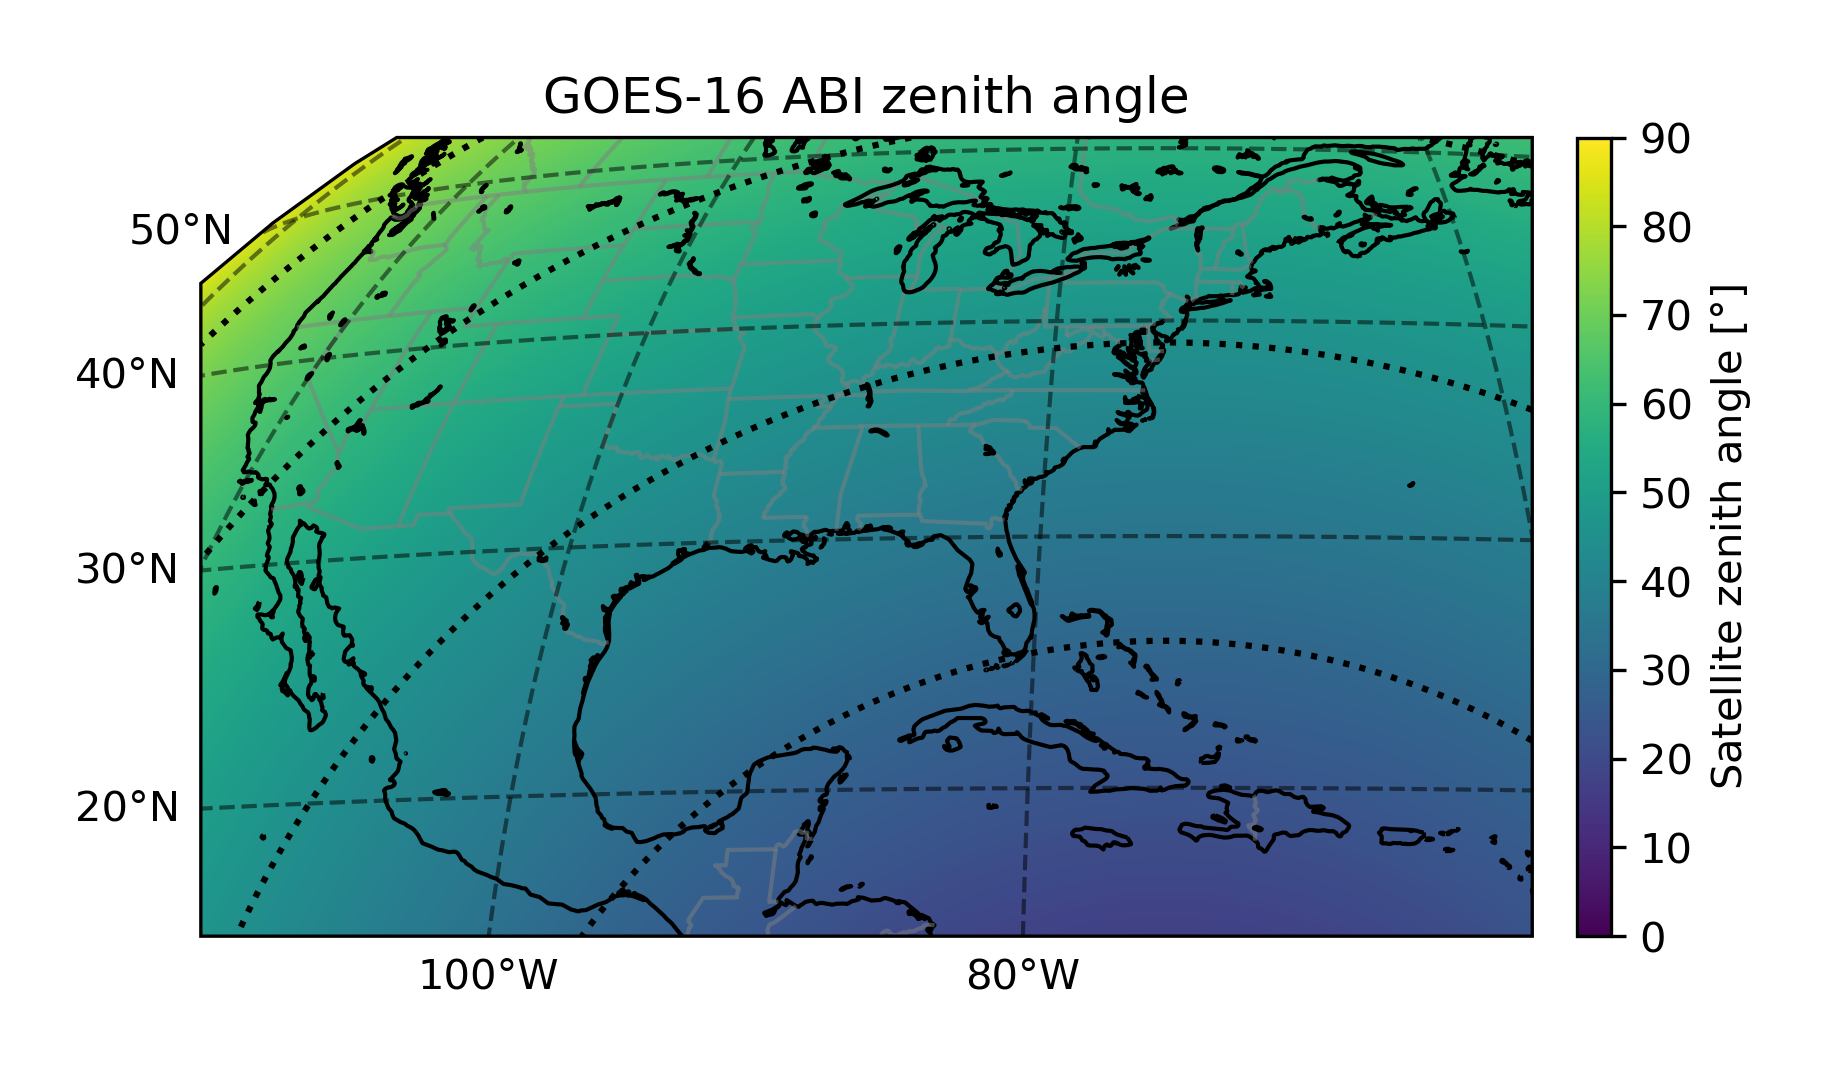
\includegraphics[width=\textwidth]{figures/chapter2_01.png}
    \caption[
    The sensor zenith angle of \acrshort{goes}-16 \acrshort{abi} observations across the \acrshort{conus} domain
    ]{
    The sensor zenith angle of \acrshort{goes}-16 \acrshort{abi} observations across the \acrshort{conus} domain. Dotted arcs are shown for each 15\,\textdegree interval of zenith angle.
    }
    \label{fig:abi_zenith_angles}
\end{figure}

To detect and track \acrshort{dcc}s across North America, \acrshort{abi} \acrshort{mcmip} data from the 6.2, 7.3, 10.4 and 12.4\,\unit{\mu m} channels observed in the \acrshort{conus} region is used, as described in section \ref{sec:abi_data}.
These observations span the full extent of the \acrshort{abi} \acrshort{conus} domain of 2,500~pixels E--W by 1,500~pixels N--S.
This domain covers a region of around 60--120\,\textdegree W in longitude and 15--50\,\textdegree N in latitude, covering an area of approximately 5,700 by 3,900\,\unit{km}.
Figure~\ref{fig:abi_zenith_angles} shows the satellite zenith angle of \acrshort{abi} observations across the \acrshort{conus} domain.
As the viewing angle increases the accurate detection and tracking of \acrshort{dcc}s becomes more difficult.
This is due to the confounding between vertical and horizontal motion, and also due to the area of each pixel increasing with the zenith angle.
The large sensor zenith angles in the North-West of the domain may introduce large errors in the detection and tracking algorithm, and so for the rest of this chapter only those \acrshort{dcc}s detected east of 110\,\textdegree W and south of 45\,\textdegree N are included in the analysis.

Five full years of data---from the start of 2018 to the end of 2022---are used to produce a dataset of detected \acrshort{dcc}s and their properties.
This period spans all complete years of operational data from \acrshort{goes}-16 \acrshort{abi}.
To improve to continuity of observations a gap-filling procedure is implemented.
If time gaps between observations of greater than 15 minutes are present, observations from the full-disc \acrshort{abi} scan are used to fill these gaps.
Full disc imagery is typically available every 10 or 15 minutes depending on the operating mode.
This gap filling is particularly important during the periods in which \acrshort{abi} uses its mode 4 scan pattern, in which no \acrshort{conus} domain scans are made, but the full-disc is scanned every 5 minutes.
Using the full-disc observations allows us to maintain temporal sampling throughout these periods.


\section{Method} \label{sec:conus_method}

Detection and tracking of convective cores and anvil cloud is performed using the \textit{tobac-flow} method \citep{jones_semi-lagrangian_2023} described in section~\ref{sec:tracking_method}.
Initial detection of \acrshort{dcc}s is performed separately over 24-hour periods spanning from 12:00:00~\acrshort{utc} (approximately 6am local time over North America) to the same time the next day.
This 24-hour period was dictated due to performance constraints, as the large domain combined with the high spatial and temporal resolution of \acrshort{abi} data results in a large memory requirement.
The start time corresponds with the minima of convective activity over land, and so was chosen in order to minimise the number of \acrshort{dcc}s missed at the start and end of the detection period.
Each period is extended by six \acrshort{abi} observations at each end to ensure at least one hour of overlap between successive days.

To track long-lived \acrshort{dcc}s that last beyond one day, a linking algorithm is used to combine \acrshort{dcc}s observed across multiple days.
The linking algorithm combines \acrshort{dcc}s detected at the same locations within the overlap period of two daily detection files.
Splitting and merging of objects is taken into account, so a single object which splits into two, or two objects which merge into one in the subsequent file are all considered a single, tracked object.
The linking algorithm is applied separately to each month of data for performance reasons.

%t
\begin{table}[b]
\centering
\begin{tabular}{ll}
\tophline
Core removed if:                                                    & Core invalid if: \\
\middlehline
Initial \acrshort{bt} -- final \acrshort{bt} \textless~8\,\unit{K}  & Intersects edge of domain \\
Lifetime \textless~15~minutes                                       & Intersects start of domain \\
Time gaps \textgreater~15~minutes                                   & Intersects end of domain \\
Maximum area \textgreater~10,000\,\unit{km\textsuperscript{2}}      & Adjacent to bad \acrshort{abi} data \\
Any NaN values in core properties                                   & \\
\bottomhline
\end{tabular}
\caption[
Validity criteria for detected cores
]{
Validity criteria for detected cores. Cores which flag any of the removal criteria are removed in their entirety from the dataset. Those which flag any of the invalid criteria are retained, but removed from subsequent analysis.}
\label{table:core_validity_criteria}
\end{table}

After linking, a processing step is applied to calculate the properties of detected cores and anvils at each step of their lifecycles.
Finally, core and anvil step properties are aggregated over each month of observation, and overall core and anvil properties are calculated.
During this final step quality flagging is performed to isolate detected features that fail one or more quality checks.
The quality criteria are split into two groups.
The first set of criteria---for core or anvil removal---removes features that cannot be verified as correctly tracked \acrshort{dcc}s due to bad data or a failure to meet the basic requirements for tracking described in chapter~\ref{chp:tracking_method}.
This may happen because there are large time gaps in the dataset, or missing data due to artifacts in the \acrshort{abi} observations.
Detected features which flag any of these criteria are removed from the aggregated dataset in their entirety.
This step in particular removes anvils which have no cores associated with them, or are not detected as initiating with a developing core.

The second set of criteria is used to identify detected cores or anvils which are not observed over their entire extent or lifecycle.
Cores and anvils which flag are of these criteria are still included within the aggregated properties dataset, but are removed from the analysis \acrshort{dcc} properties throughout this chapter.
Quality criteria for cores are listed in table \ref{table:core_validity_criteria}, and those for anvils in table \ref{table:anvil_validity_criteria}.


%t
\begin{table}[tb]
\centering
\begin{tabular}{ll}
\tophline
Anvil removed if:                               & Anvil invalid if: \\
\middlehline
No associated cores                             & Intersects edge of domain \\
Lifetime \textless~15~minutes                   & Intersects start of domain \\             
Time gaps \textgreater~15~minutes               & Intersects end of domain \\
Maximum area \textless~maximum core area        & Adjacent to bad \acrshort{abi} data \\
Anvil detected before initial core              & Associated with invalid cores \\
Anvil dissipated before final core ends         & Maximum area reached before end \\
Any NaN values in anvil properties              & ~~of initial core \\
\bottomhline
\end{tabular}
\caption[
Validity criteria for detected anvils
]{
Validity criteria for detected anvil. Anvils which flag any of the removal criteria are removed in their entirety from the dataset. Those which flag any of the invalid criteria are retained, but removed from subsequent analysis. The majority of anvils removed are due to have no associated cores, or because the anvil was observed before any developing cores.}
\label{table:anvil_validity_criteria}
\end{table}


The complete processing pathway is outlined by the following steps:

\begin{enumerate}
    \item Detection of cores and anvils in \acrshort{abi} observations over each 24-hour period.
    \item Linking of overlapping objects detected in subsequent 24-hour periods over each month.
    \item Calculation of core and anvil step properties. 
    \item Quality criteria applied to core and anvils, properties aggregated over each month
\end{enumerate}

Two datasets are produced. The first consists of daily core and anvil spatial maps, with step properties, produced by processing step 3. 
The second, consisting of aggregated monthly core and anvil properties, is produced by step 4.

\begin{figure}[tp]
    \centering
    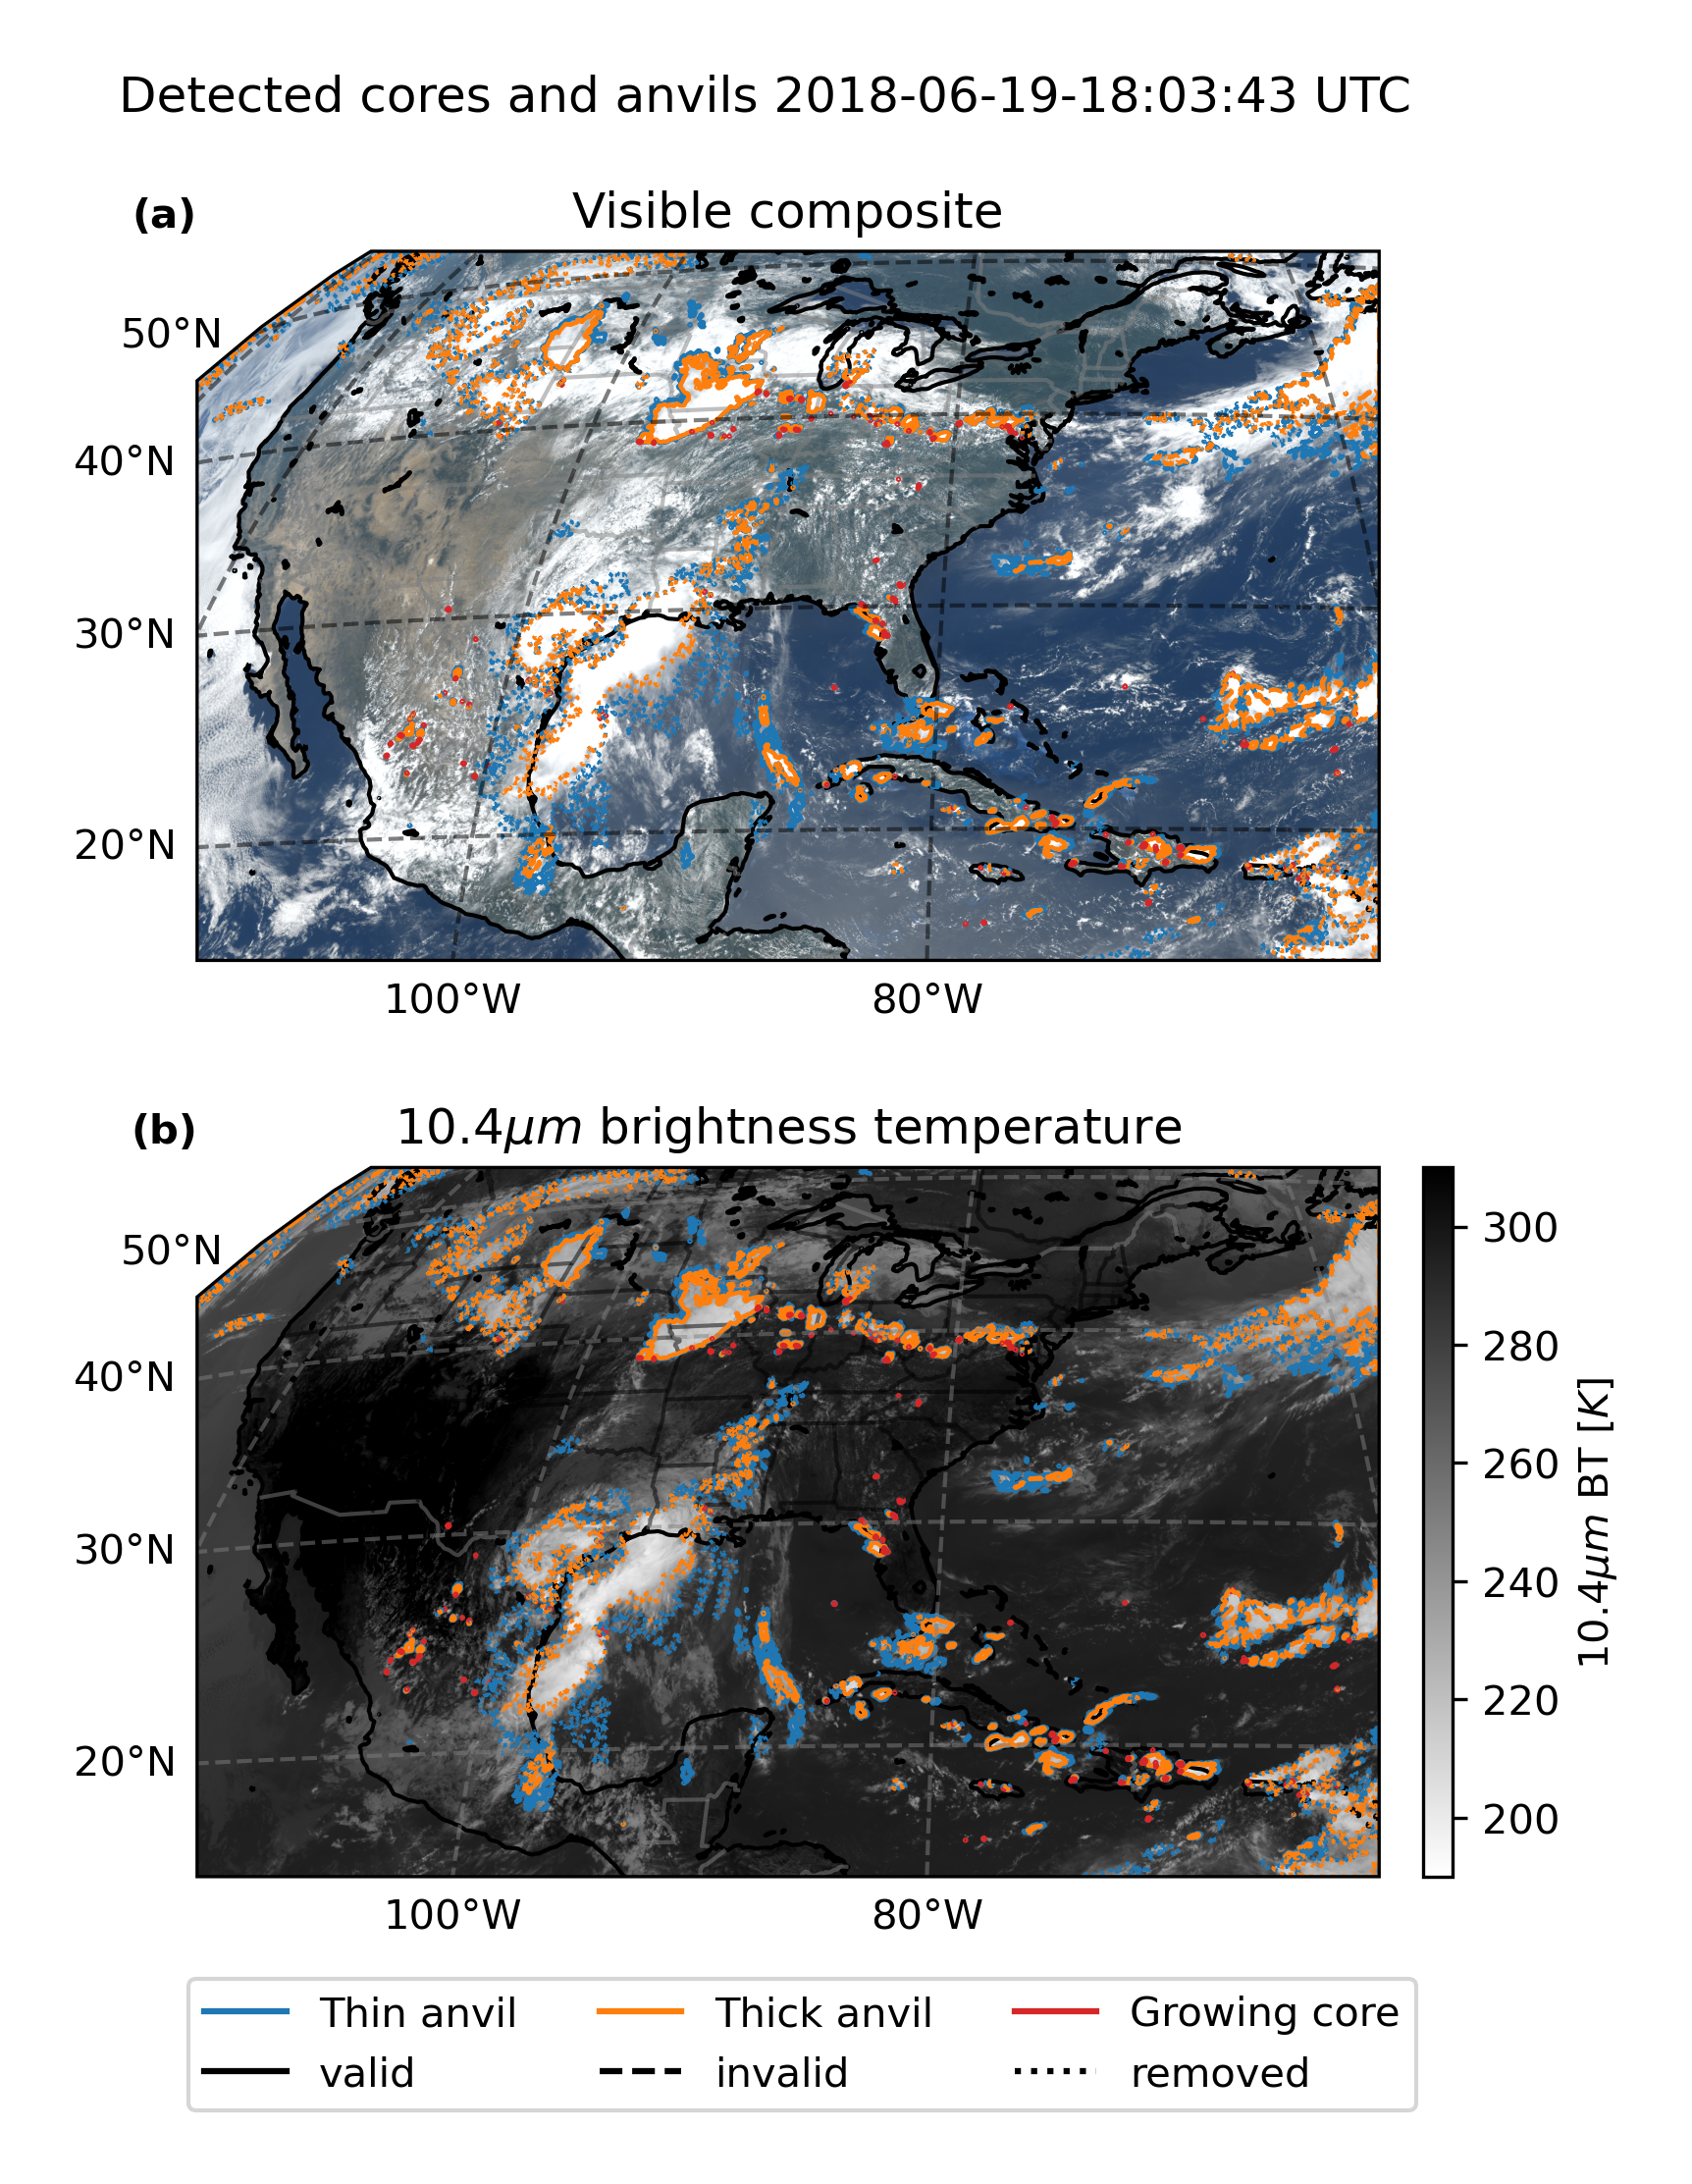
\includegraphics[width=\textwidth]{figures/chapter2_02.png}
    \caption[
    Detected cores and anvils from a snapshot of \acrshort{goes}-16 \acrshort{conus} domain observations
    ]{
    Detected cores and anvils from a snapshot of \acrshort{goes}-16 \acrshort{conus} domain observations. Cores and anvils removed from the aggregated dataset are shown with dotted outlines. Those which are flagged as invalid are shown with dashed outlines. Detected features are shown against (a) visible composite imagery and (b) 10.4\,\unit{\mu m} \acrshort{bt}
    }
    \label{fig:conus_detected_dccs}
\end{figure}

Figure~\ref{fig:conus_detected_dccs} shows an example of detected cores and anvils over the \acrshort{conus} region, against backgrounds of composite visible imagery (fig.~\ref{fig:conus_detected_dccs}\,a) and 10.4\,\unit{\mu m} \acrshort{bt} (fig.~\ref{fig:conus_detected_dccs}\,b).
Cores and anvils which are removed from the aggregated dataset are outlined with dotted lines, and those which are marker invalid are shown with dashed outlines.
The large, organised convective system centred at 95\,\textdegree W, 27\,\textdegree N has been removed as it is intersected by a scan-line artifact later in its lifetime.
The \acrshort{dcc}s observed along the eastern edge of the domain have been marked invalid as, while they are considered true detections of \acrshort{dcc}s, they intersect the edge of the domain.

Over the five-year observing period a total of 3,877,130 cores are detected, of which 3,615,533 are consider valid, and 1,643,030 are linked with an anvil cloud. 
A total of 648,345 anvils are detected, of which 391,050 are valid, and these valid anvils contain 792,522 cores.
The disparity in the number of valid cores and the number of cores contained with valid anvils is due to additional filtering applied to the anvils.
As the larger and longer-lived anvils are more likely to intersect the edges of the domain, they are more likely to be marked invalid than the cores.
In these cases, the cores themselves are valid for analysis, as their evolution is observed in its entirety, but exclude the anvil itself from analysis as we do not capture its entire extent and lifetime.
The exclusion of anvils that intersect the edges of the domain introduces a bias towards removing larger, long-lived systems near the edge of the domain, which should be considered when assessing the properties of the observed \acrshort{dcc}s.


\section{Results}


\subsection{Distributions and properties of developing convective cores} \label{sec:core_properties}

%f
\begin{figure}[tp]
    \centering
    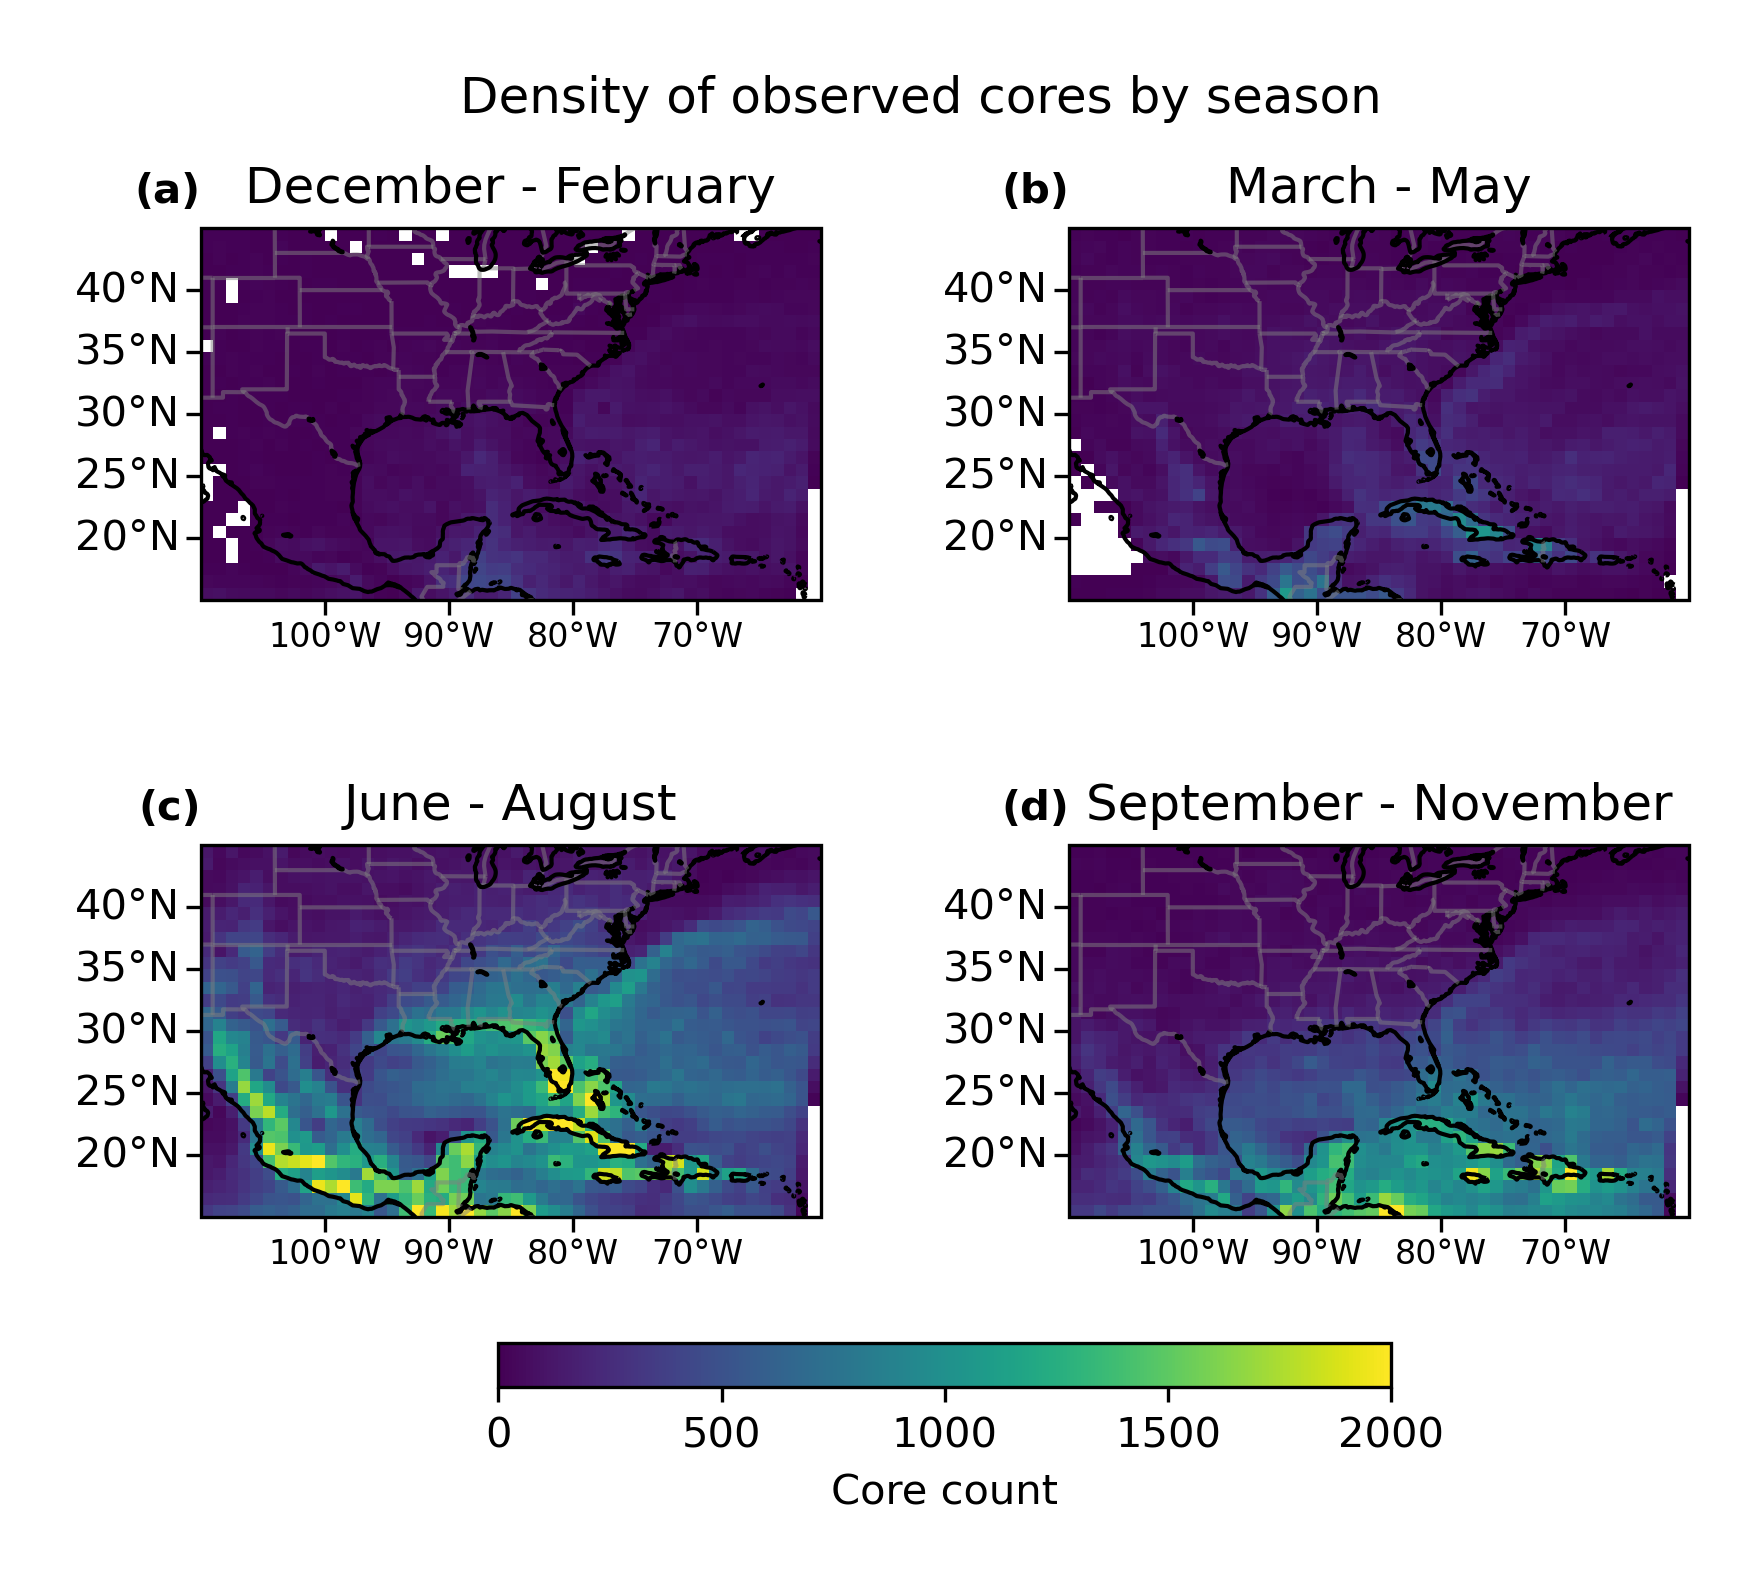
\includegraphics[width=\textwidth]{figures/chapter2_03.png}
    \caption[
    The spatial distribution of observed cores by season
    ]{
    The spatial distribution of observed cores, broken down by season and accumulated into 1\texttimes1\textdegree\ grid boxes of latitude and longitude. The density of observed cores is greatest during summer (c) and smallest during winter (a).
    }
    \label{fig:core_density_by_season}
\end{figure}

To begin, the distribution of detected \acrshort{dcc} cores throughout the dataset is investigated.
Figure~\ref{fig:core_density_by_season} shows the distribution of observed cores over North America separated by season.
Large variations in the spatial distribution of cores can be observed across the different seasons.
Overall, in winter and spring (fig.~\ref{fig:core_density_by_season}\,a,b) there are lower rates of observed \acrshort{dcc}s than in the summer and autumn (fig.~\ref{fig:core_density_by_season}\,c,d).

In winter (fig.~\ref{fig:core_density_by_season}\,a) the majority of convection observed occurs over the ocean, particularly in the areas of the Gulf of Mexico and West Atlantic associated with warm currents.
In spring (fig.~\ref{fig:core_density_by_season}\,b), a similar pattern shows over the ocean, and there is also an increase in convection detected over land in the Caribbean, Mexico and the central and southern \acrshort{usa}.
In summer (fig.~\ref{fig:core_density_by_season}\,c) there is a large increase in convection over land and ocean, with the highest rates of convection of any season.
There are, in particular, high rates of convection over Mexico, the Caribbean, the southern \acrshort{usa} (Florida in particular) and adjacent ocean regions.
In Autumn (fig.~\ref{fig:core_density_by_season}\,d) there is a large reduction in the number of convective cores detected over land regions.
The number of detections over the ocean remains high, however, indicating a possible lag in the seasonal cycle of convection over oceans compared to that over land.

%f
\begin{figure}[tp]
    \centering
    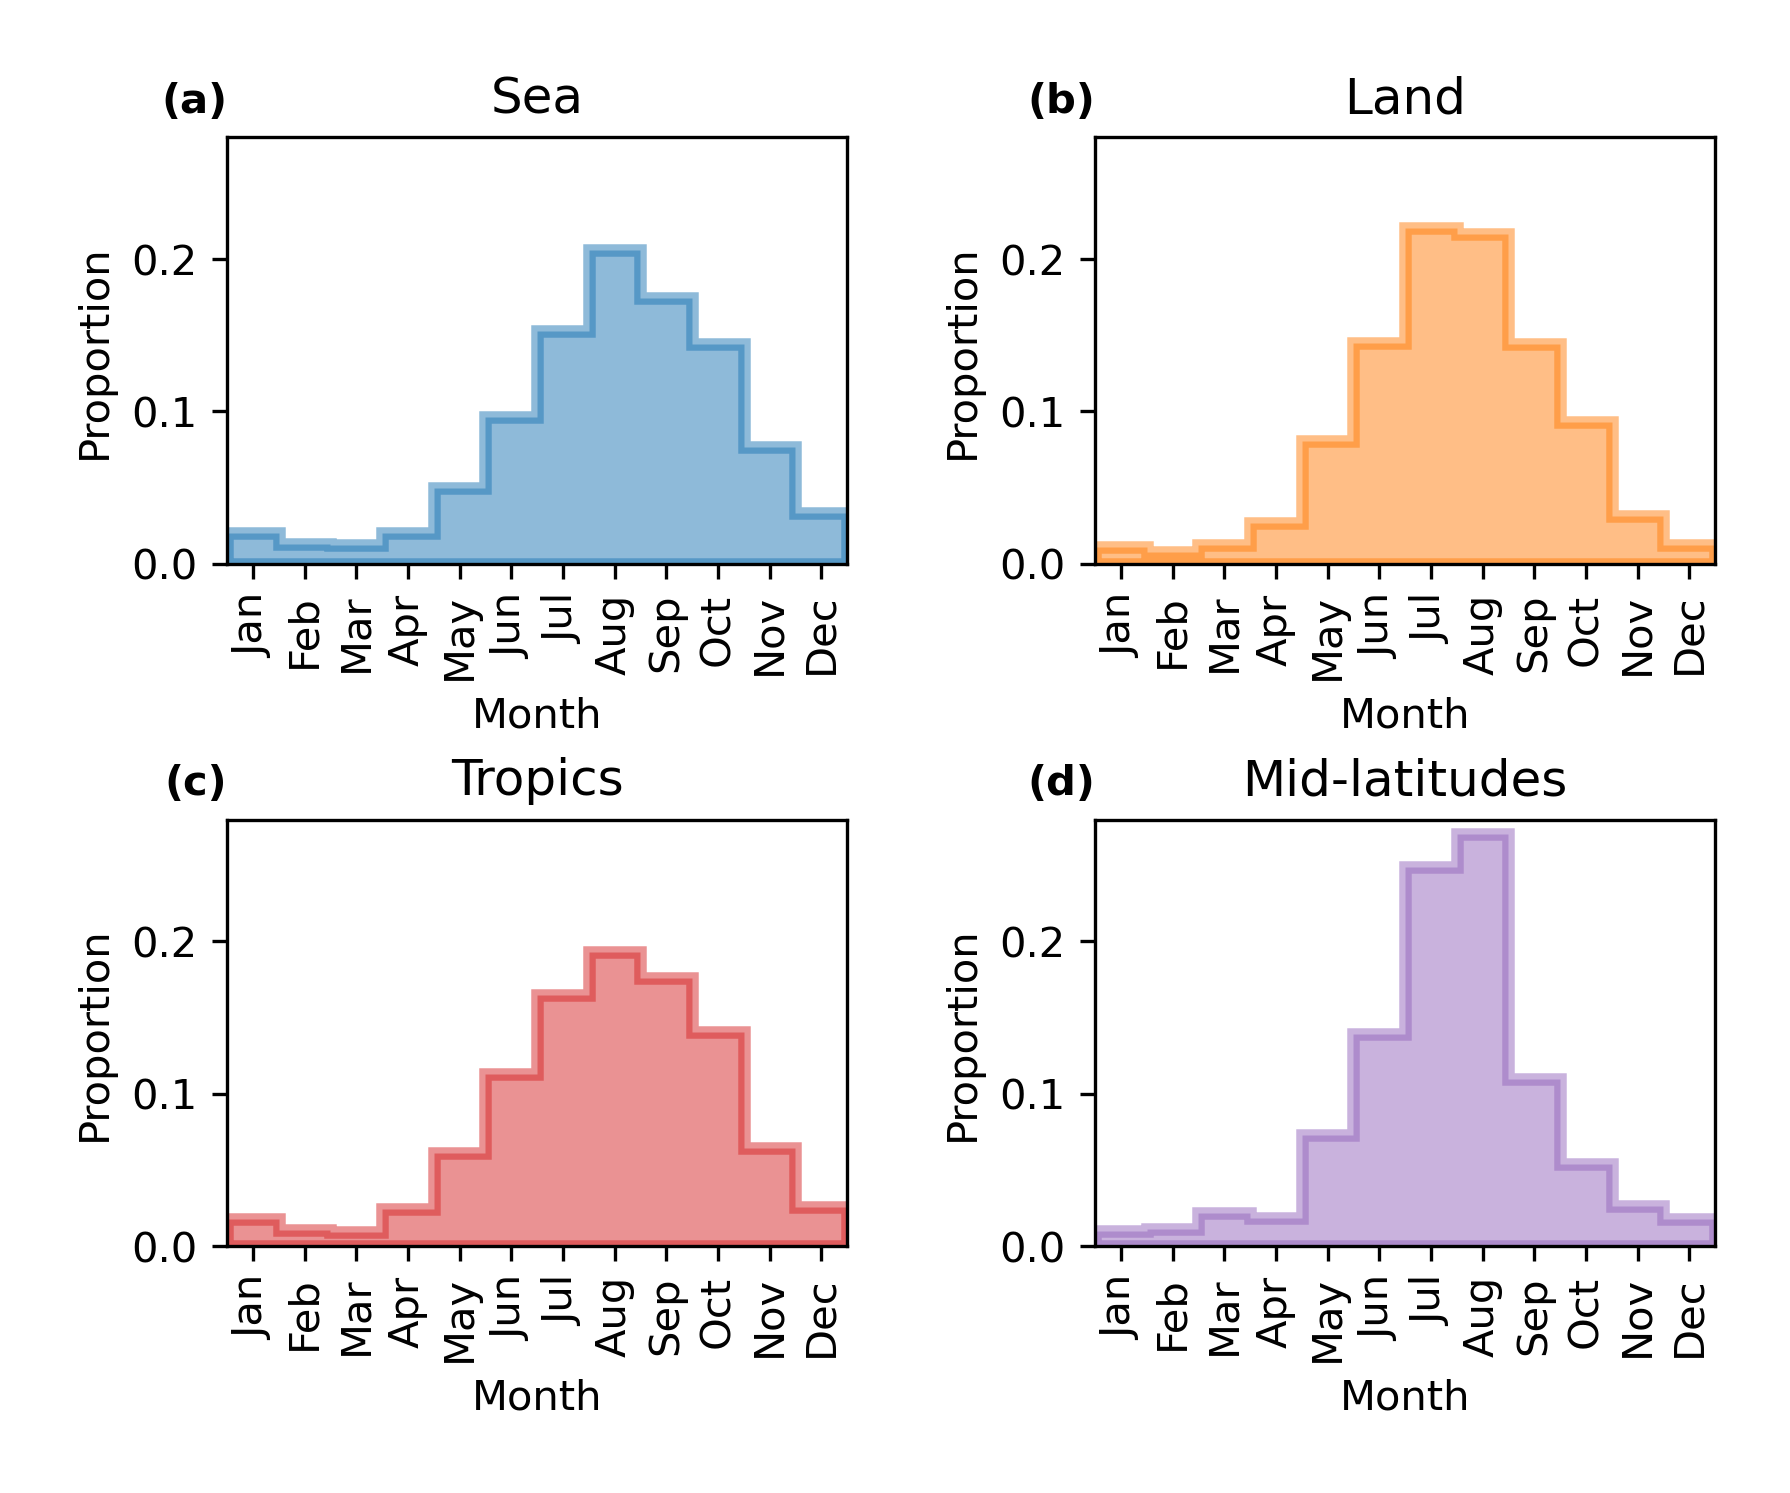
\includegraphics[width=\textwidth]{figures/chapter2_04.png}
    \caption[
    Monthly distributions of the proportion of cores detected each month over land, sea, tropics and mid-latitudes
    ]{
    Monthly distributions of the proportion of cores detected each month over (a) sea, (b) land, (c) tropics (\textless 30\,\textdegree N) and (d) mid-latitudes (\textgreater 30\,\textdegree N).
    }
    \label{fig:core_annual_land_sea}
\end{figure}


Figure~\ref{fig:core_annual_land_sea} shows the proportion of cores detected in each month over the annual cycle for land and sea regions.
Both land and sea regions show a peak of convective activity in the summer, and a low in the winter months.
However, as suggested by fig.~\ref{fig:core_density_by_season}, there is a time lag of about 1 month between the annual cycle of convection over land and that over the ocean, likely due to the time lag in ocean heating.
Comparing the tropics and mid-latitudes, the monthly distribution of convection is much more sharply focused on July--August in the mid-latitudes compared to the broader distribution seen in the tropics.


%f
\begin{figure}[tp]
    \centering
    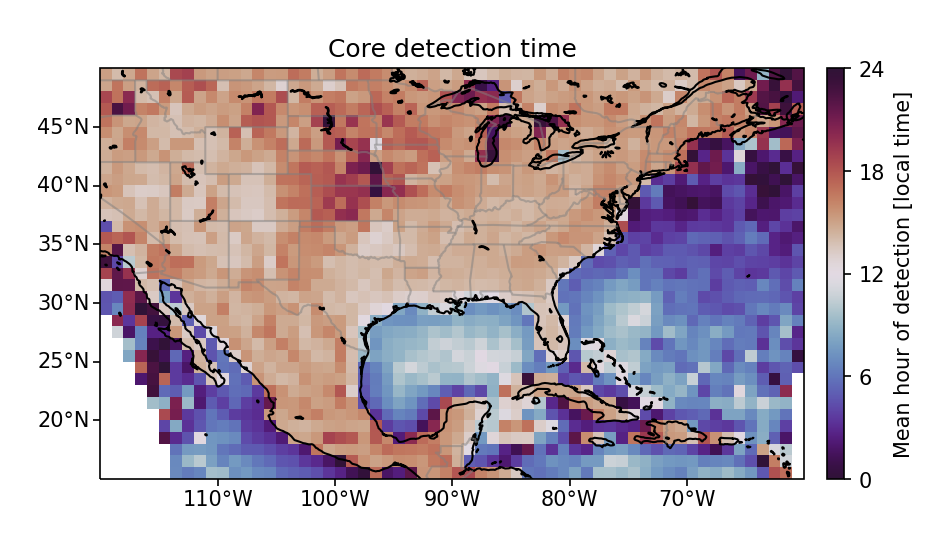
\includegraphics[width=\textwidth]{figures/chapter2_05.png}
    \caption[
    The average speed and direction of propagation of cores
    ]{
    The average speed and direction of propagation of cores observed within each 1\texttimes1\textdegree\ grid box. The colouring shows the average speed of propagation, and the red arrows show the average direction for each 2\texttimes2\textdegree\ grid box}
    \label{fig:core_propagation_map}
\end{figure}

Figure~\ref{fig:core_propagation_map} shows the average speed of propagation for cores observed in each 1-degree grid box, with the average direction of propagation shown by arrows for each 2-degree grid box.
There is a clear change in the direction of propagation from an easterly motion in the tropics (below 25\,\textdegree N) to a south-westerly motion in the mid-latitudes.

%f
\begin{figure}[tp]
    \centering
    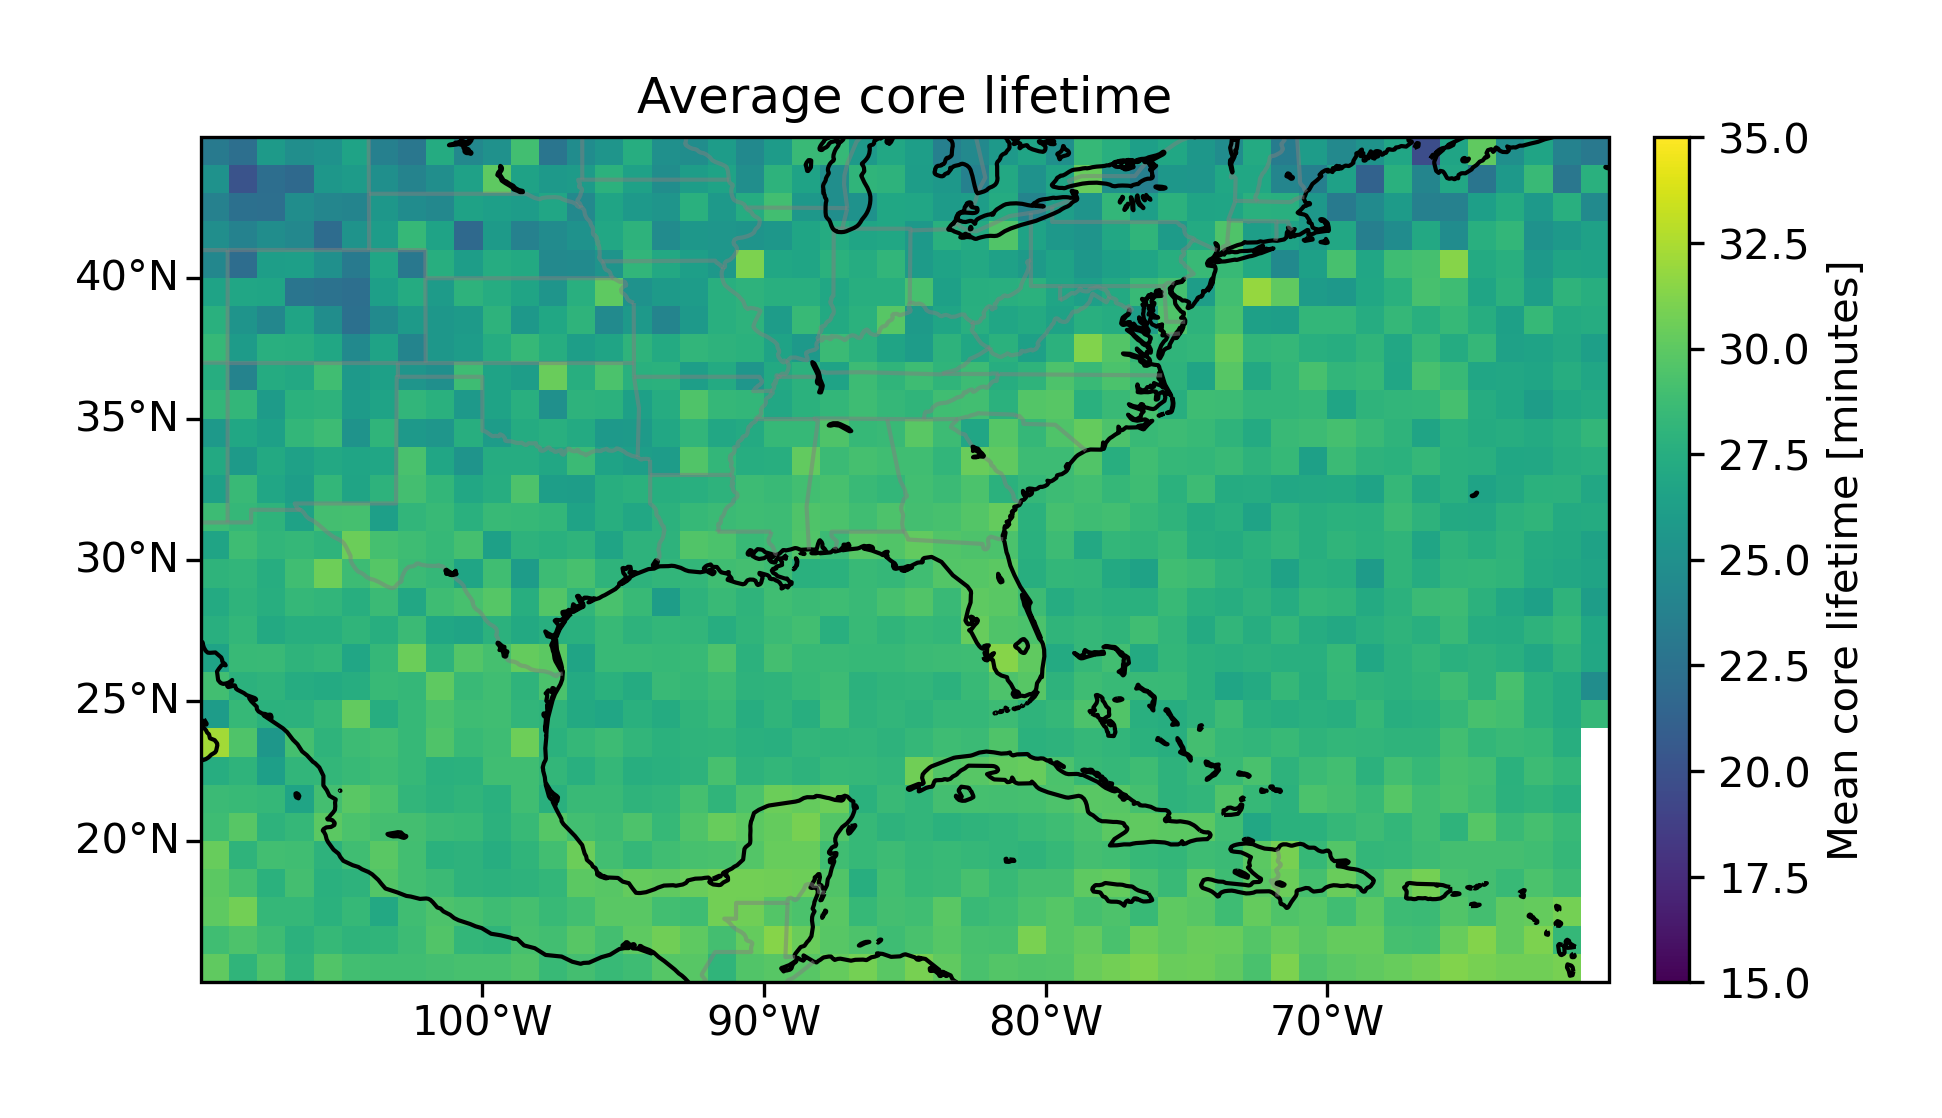
\includegraphics[width=\textwidth]{figures/chapter2_06.png}
    \caption[
    A map showing the mean lifetime in minutes of cores within each 1\texttimes1
    \textdegree\ grid box
    ]{
    A map showing the mean lifetime in minutes of cores within each 1\texttimes1
    \textdegree\ grid box.
    }
    \label{fig:core_lifetime_map}
\end{figure}

Figure \ref{fig:core_lifetime_map} displays the mean lifetime of observed cores over each 1-degree box of latitude and longitude.
The lifetime is defined as the period of time over which each core is detected, which represents the time in which to core is developing vertically.
Convection will continue in the core after this point, but the motion of the cloud top will instead be a horizontal divergence of the anvil.
The average lifetimes appear mostly uniform across the domain, with a small reduction with increasing latitude.
This reduction in the lifetime of the developing core at higher latitudes is likely due to the lower tropopause height restricting the vertical development of the cores.
Similarly, there is a slight reduction in average lifetime over the more mountainous, inland regions of Mexico compared to the adjacent coastal regions.
This again may be linked to the reduction in the depth of the convective cores, although in this case due to an increased surface height rather than a lower tropopause.


%f
\begin{figure}[tp]
    \centering
    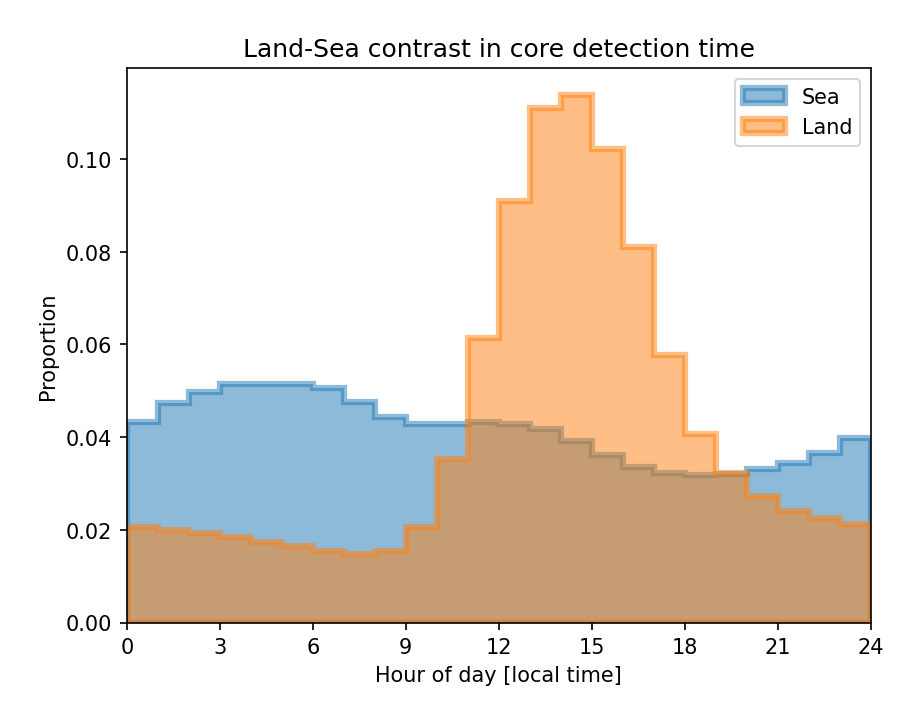
\includegraphics[width=\textwidth]{figures/chapter2_07.png}
    \caption[
    A map of the average maximum core cooling rate for each 1\texttimes1
    \textdegree\ grid box
    ]{
    A map of the  average maximum core cooling rate for each 1\texttimes1
    \textdegree\ grid box.
    }
    \label{fig:core_cooling_rate_map}
\end{figure}

Figure~\ref{fig:core_cooling_rate_map} shows the average cooling rate of observed cores.
The contrasts here are more pronounced that those shown in fig.~\ref{fig:core_lifetime_map}.
There is a reduction in the average cooling rate with latitude, likely due to the reduction in solar heating and hence lower \acrshort{cape}.
Orography also has a factor, with lower cooling rates observed over the mountains of Mexico and the North American Rockies.
The largest average core cooling rates are observed in in coastal regions, indicating potential land--sea interactions.

%f
\begin{figure}[tp]
    \centering
    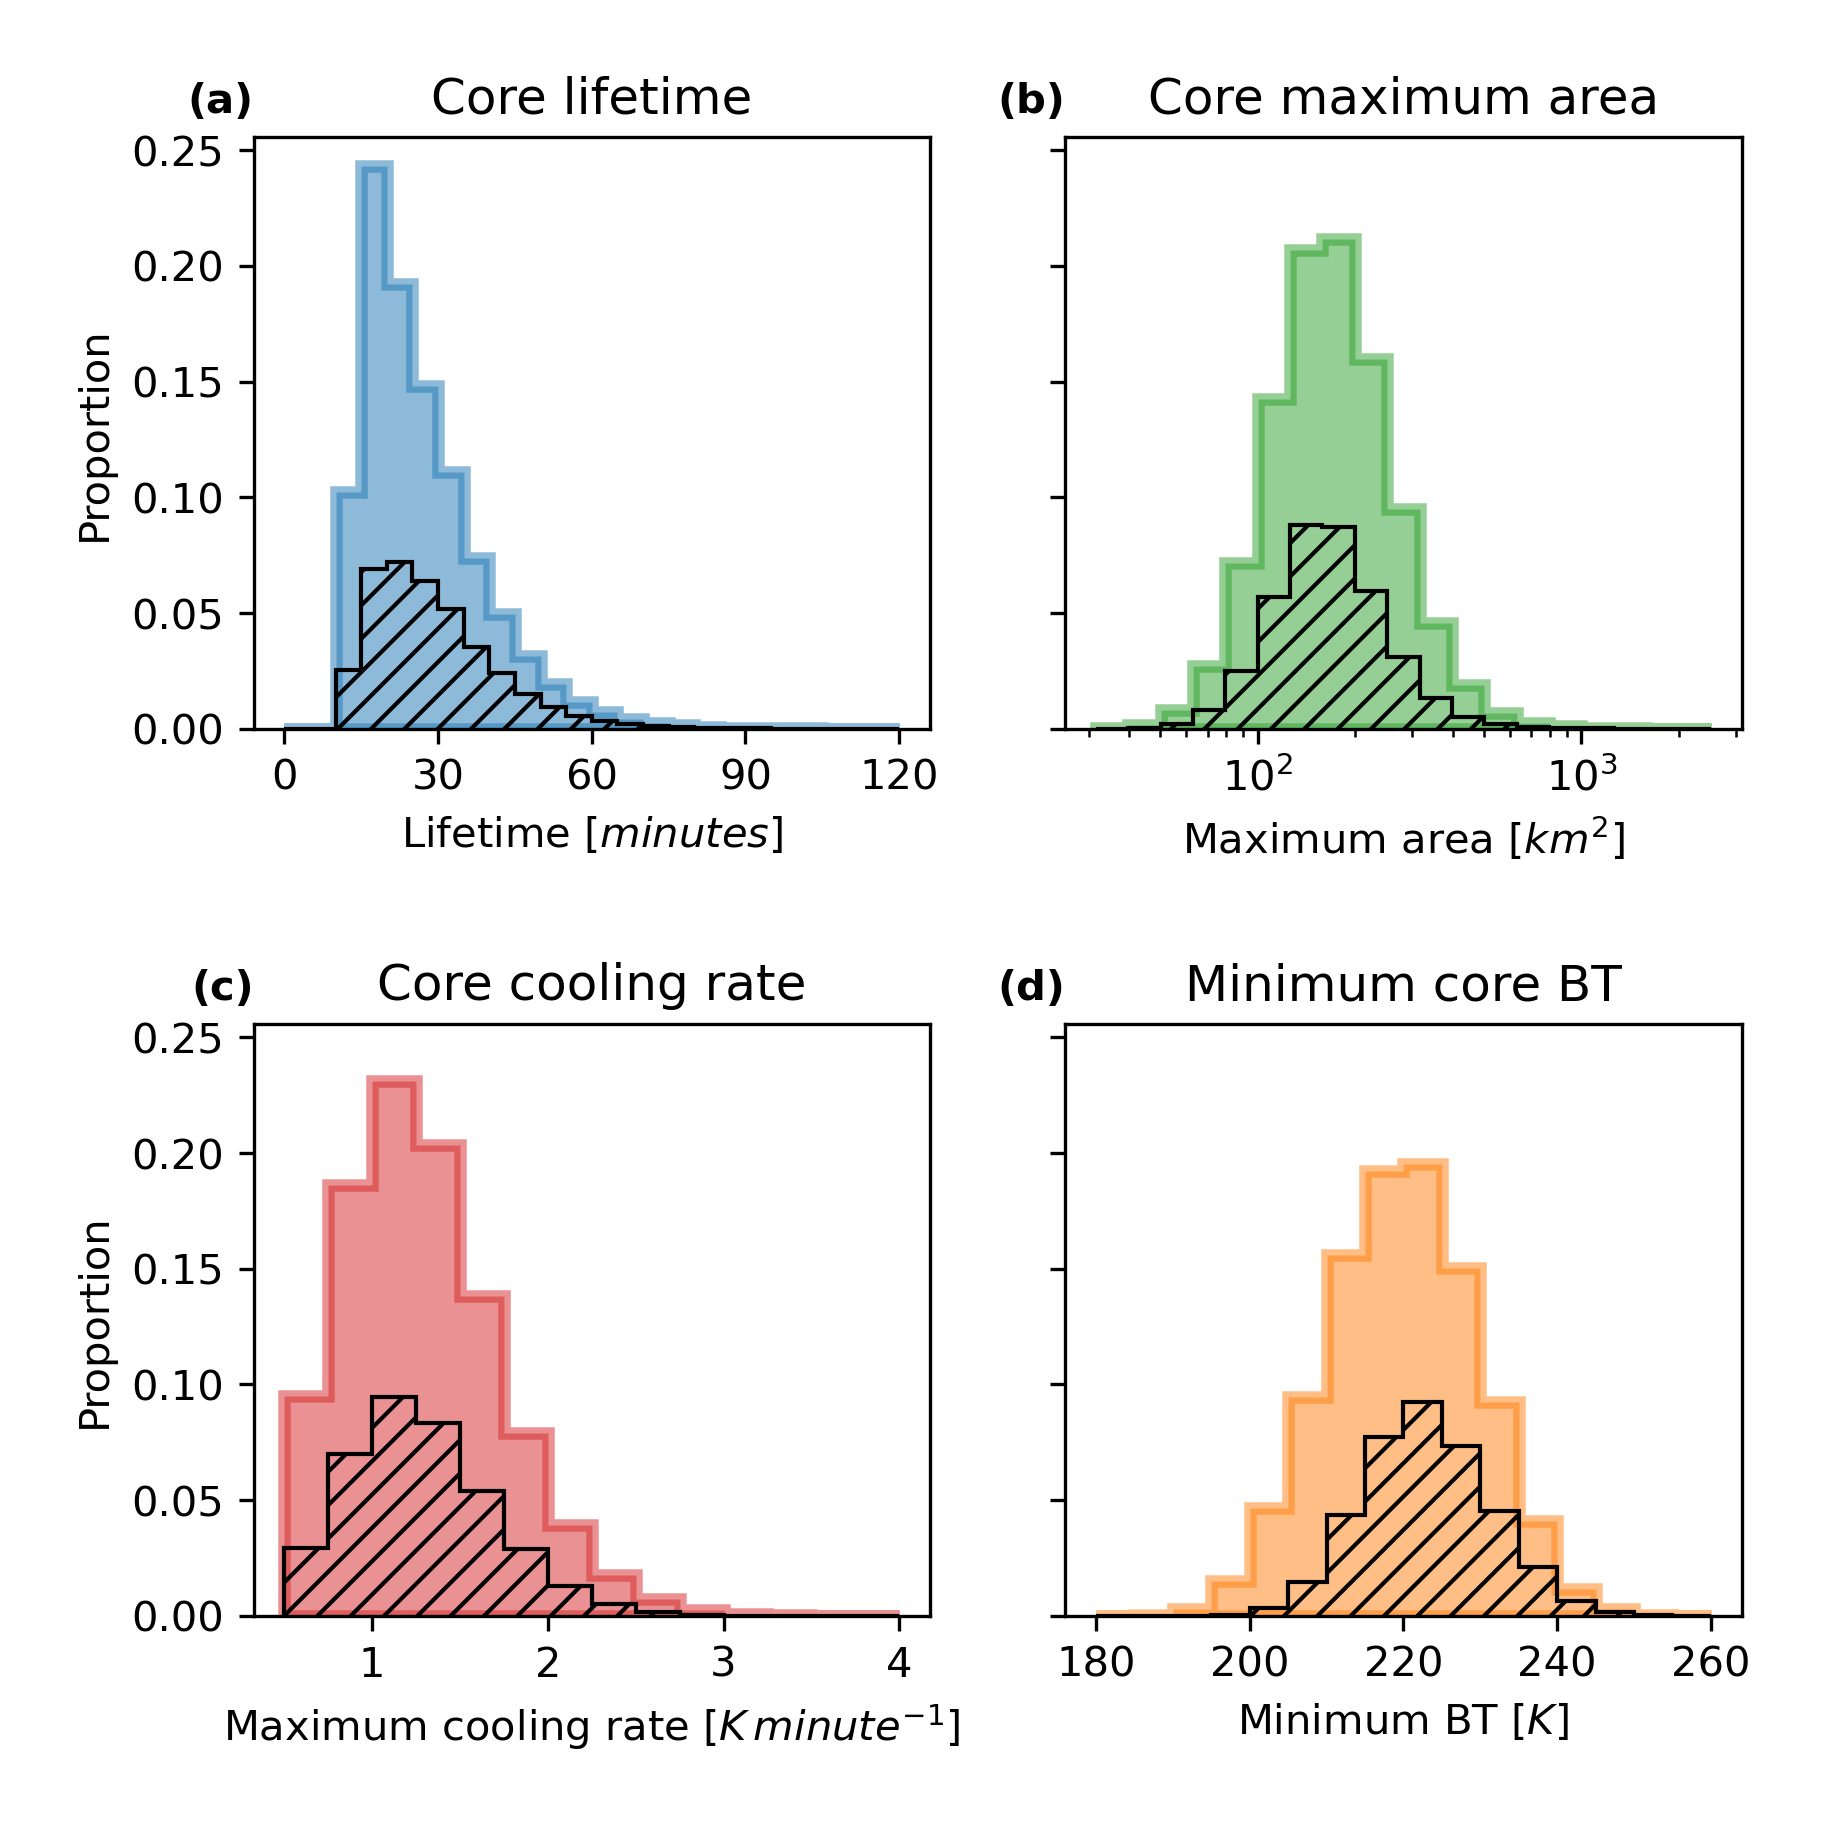
\includegraphics[width=\textwidth]{figures/chapter2_08.png}
    \caption[
    Histograms showing the distributions of observed core lifetimes, maximum areas, cooling rates and \acrshort{bt}
    ]{
    Histograms showing the distributions of observed (a) core lifetime, (b) maximum area, (c) maximum cooling rate, (d) and minimum \acrshort{bt}. The hatched areas show the proportion of each distribution consisting of the initial detected cores within each tracked \acrshort{dcc}.
    }
    \label{fig:core_properties}
\end{figure}

Figure~\ref{fig:core_properties} shows the distributions of lifetime (fig.~\ref{fig:core_properties}\,a), maximum area (fig.~\ref{fig:core_properties}\,b), cooling rate (fig.~\ref{fig:core_properties}\,c), and minimum \acrshort{bt} (fig.~\ref{fig:core_properties}\,d).
There is a peak in the observed lifetime of cores between 15 and 20 minutes, with a large tail extending beyond 60 minutes in some cases.
Note that due to the requirement of a minimum of three consecutive observations, cores lasting less than 10 minutes will not be detected, truncating the distribution.
In fig.~\ref{fig:core_properties}\,b the maximum core area peaks around 150--200\,\unit{km\textsuperscript{2}}, representing cores approximately 12--14 km in diameter.
Figure~\ref{fig:core_properties}\,c shows that the core cooling rate peaks at values of 1--1.25\,\unit{K minute\textsuperscript{-1}}, representing vertical cloud top velocities of approximately 2.5--3\,\unit{ms\textsuperscript{-1}}.
The distribution is slightly truncated by the requirement for detected cores to have a cooling rate of at least 0.5\,\unit{K minute\textsuperscript{-1}}.
Finally, the minimum core \acrshort{bt} (fig.~\ref{fig:core_properties}\,d) peaks around 220\,\unit{K}, the temperature of the radiative tropopause \citep{jeevanjee_simple_2020}

The hatched areas in fig.~\ref{fig:core_properties} show the proportion of each distribution consisting of the initial cores of tracked \acrshort{dcc}s.
For these initial cores there is no possibility of the observations being masked by an overlaying anvil cloud, these are expected to provide the most complete measurements of developing core properties.
For the lifetime, maximum area and cooling rate these show close similarities to the shape of the distribution for all cores, indicating that masking due to anvils does not significantly affect the ability to observe the core properties.
For the minimum core \acrshort{bt}, the initial cores tend to have warmer \acrshort{bt} than later cores, indicating an increased presence of cold cores and overshooting tops in organised convection.

%f
\begin{figure}[tp]
    \centering
    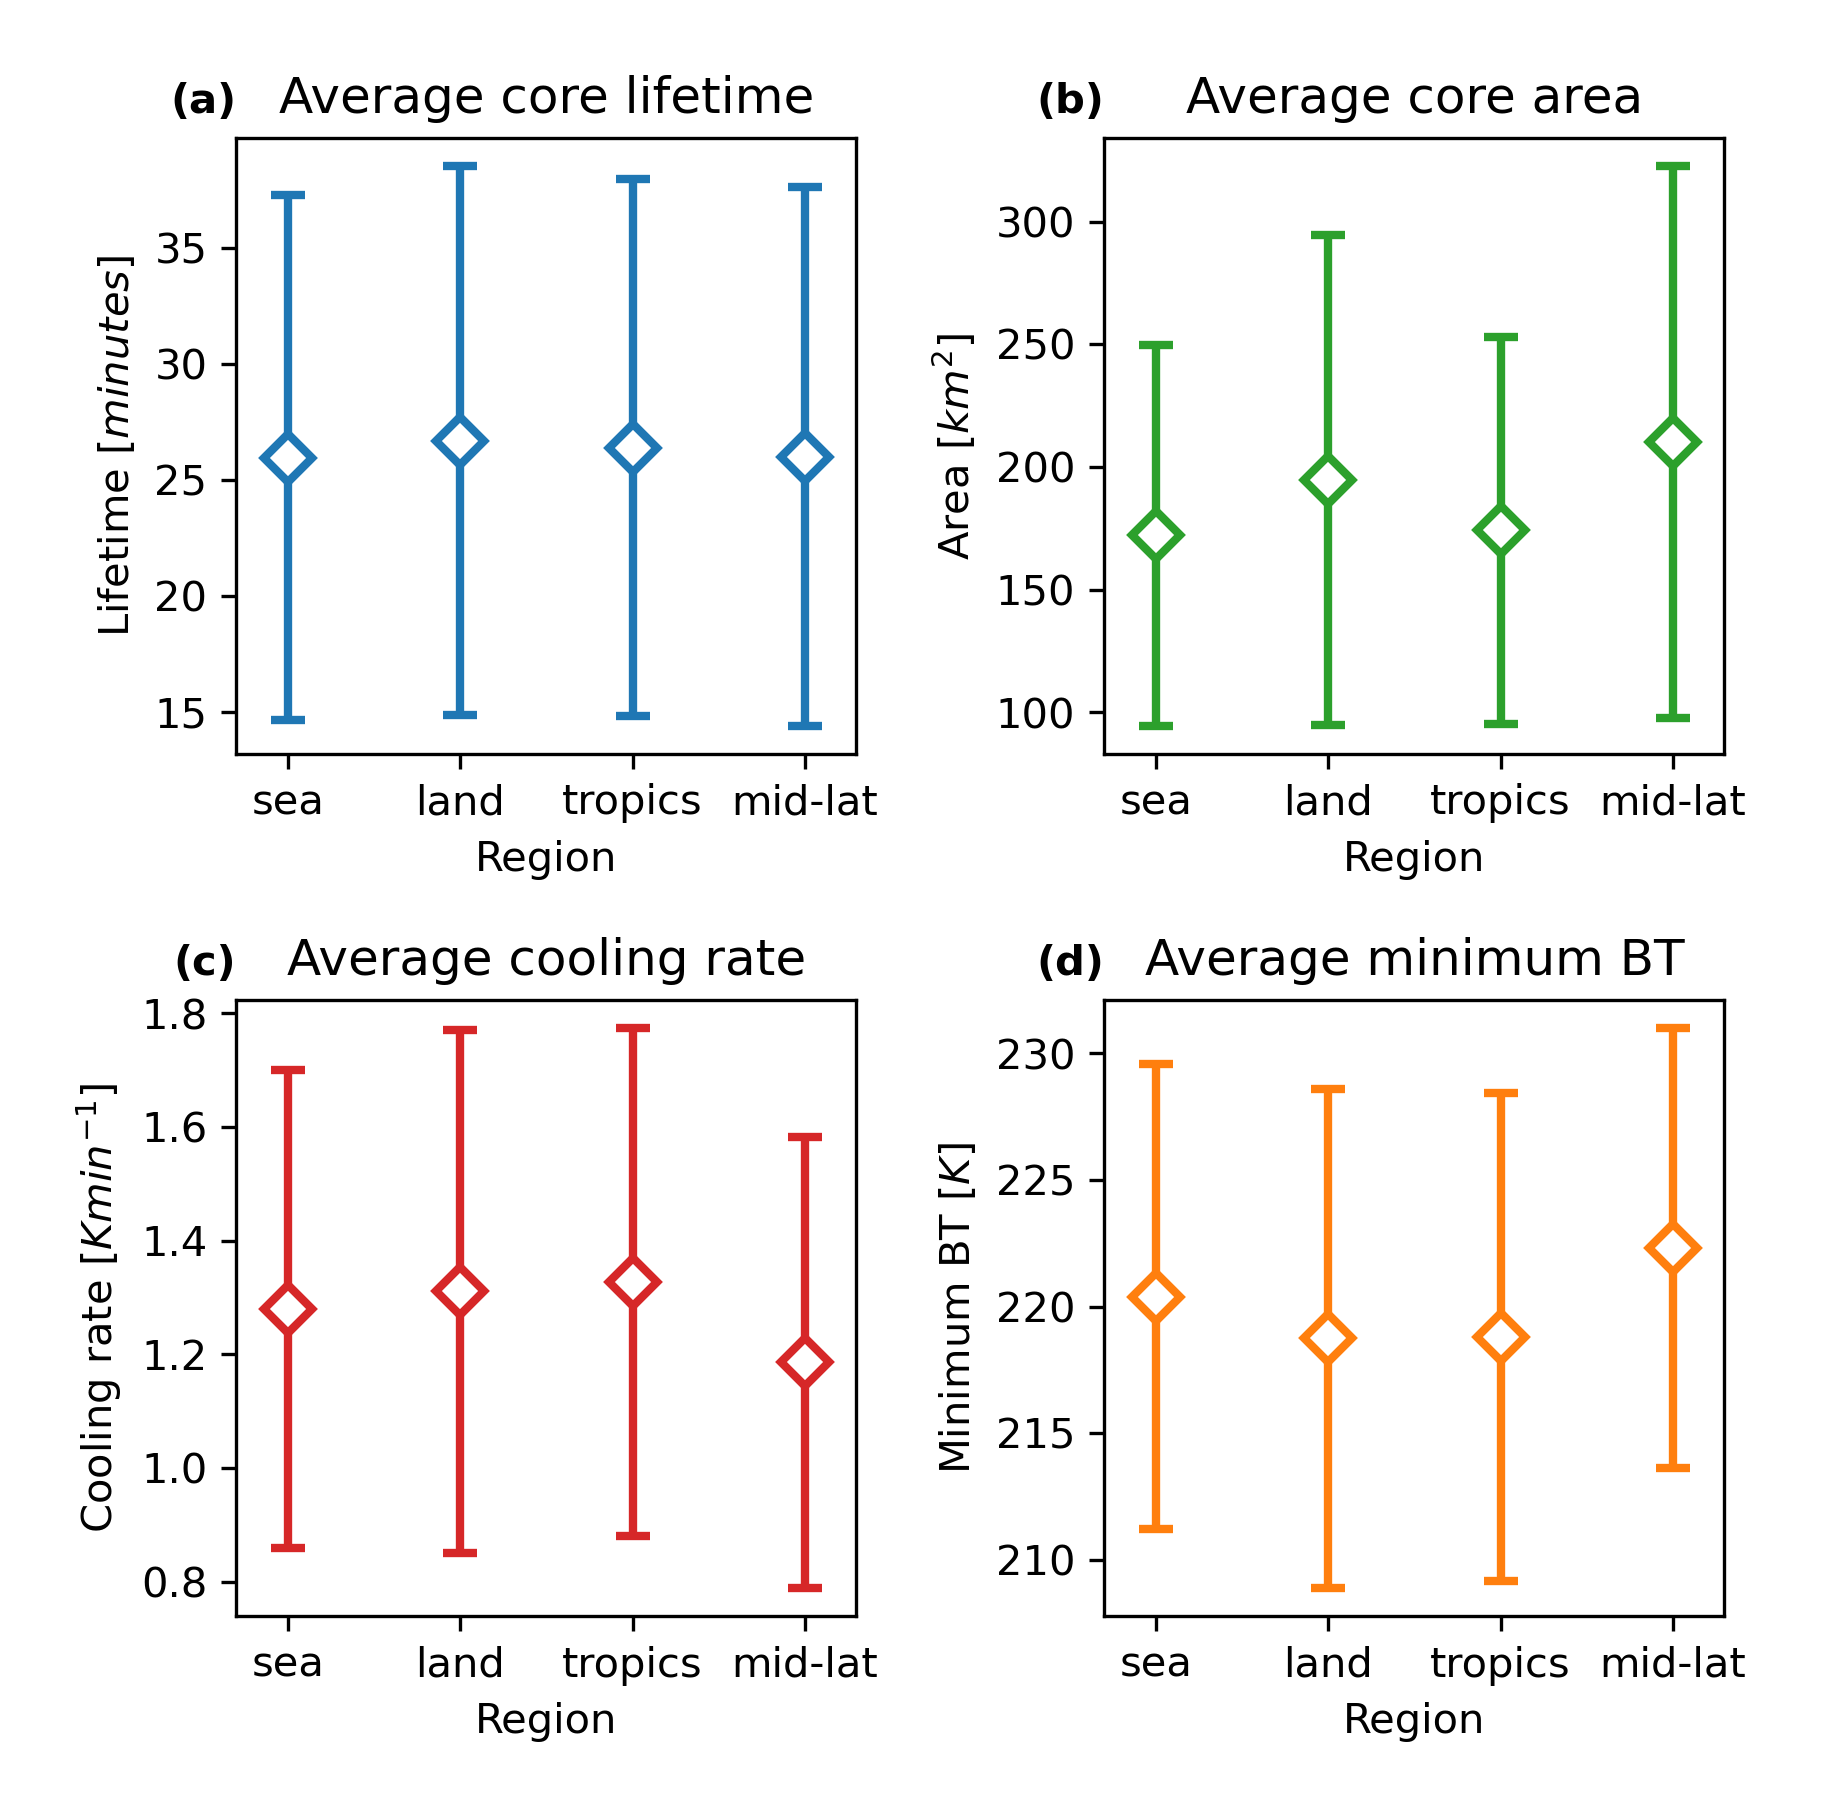
\includegraphics[width=0.75\textwidth]{figures/chapter2_09.png}
    \caption[
    The mean observed lifetimes, maximum areas, cooling rates and \acrshort{bt} for cores detected over land, sea, tropics and mid-latitudes
    ]{
    The mean observed (a) lifetime, (b) maximum area, (c) maximum cooling rate, (d) and minimum \acrshort{bt} for cores detected over land, sea, tropics and mid-latitudes. Error bars show to standard deviation of each point.
    }
    \label{fig:core_region_mean_properties}
\end{figure}

Figure~\ref{fig:core_region_mean_properties} shows how the mean core lifetime, maximum area, cooling rate and \acrshort{bt} vary between different regions.
There is little difference in the mean core lifetime between regions, echoing the results seen in fig.~\ref{fig:core_lifetime_map}.
Maximum core area is larger over land than sea, and larger in the mid-latitudes than in the tropics.
There is little difference in the cooling rate between sea and land, but on average cores in the tropics cool $\sim$0.2\,\unit{K minute\textsuperscript{-1}} faster than those in the mid-latitudes.
There is a small difference in the minimum \acrshort{bt} of cores observed over land and ocean, with the former $\sim$1.5\,\unit{K} colder than the latter.
A more noticeable difference is seen with latitude, with cores in the tropics having, on average, minimum \acrshort{bt} $\sim$5\,\unit{K} colder than those in the mid-latitudes.

Overall, fig.~\ref{fig:core_region_mean_properties} show differences in core intensity between land and ocean, and between the tropics and mid-laitudes, with these differences most prominent in the minimum \acrshort{bt}.
However, these differences may result from changes in different properties of the cores as the difference in cooling rate between tropics and mid-latitudes is not seen when comparing sea and land.

%f
\begin{figure}[tp]
    \centering
    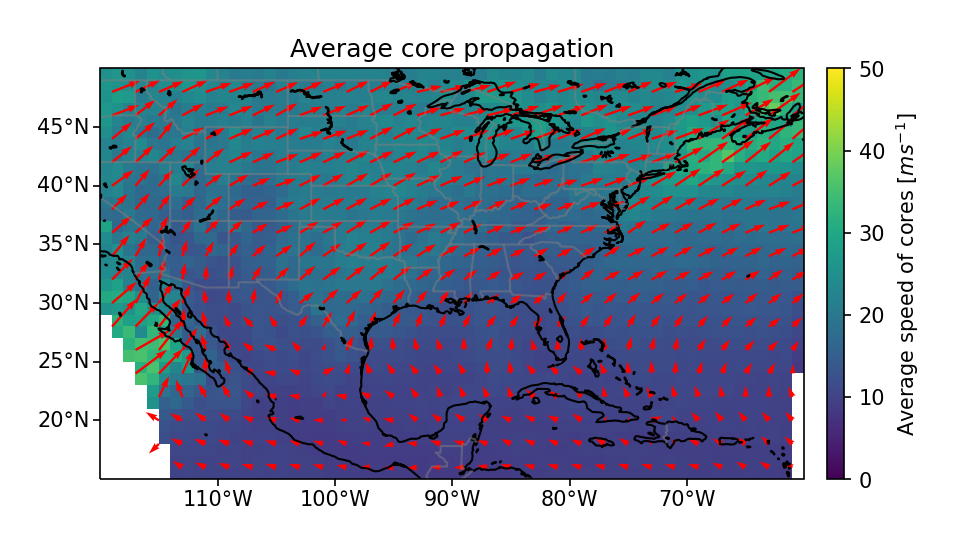
\includegraphics[width=0.75\textwidth]{figures/chapter2_10.png}
    \caption[
    Average core lifetime and minimum \acrshort{bt} with increasing core cooling rate
    ]{
    Average core lifetime (a) and minimum \acrshort{bt} (b) with increasing core cooling rate. Error bars show the variance of the data, while the shaded area shows the standard error of the mean.
    }
    \label{fig:core_cooling_rate_relations}
\end{figure}


Figure~\ref{fig:core_cooling_rate_relations}\,a compares how the average lifetime of detected cores changes with their maximum observed cooling rate.
For low values of core cooling rate, there is a similar, positive linear relationship between cooling rate and lifetime between all regions, indicating that more intense convection leads to longer periods of cores being observed.
However, beyond cooling rates of around 1.5\,\unit{K minute\textsuperscript{-1}} there is a peak in the core intensity--height relationship, with larger cooling rates leading to shorter lifetimes.
This may be explained by the cores with faster cooling rates reaching their level of neutral buoyancy faster, and therefore showing cooling cloud tops for a shorter period of time.
The inflexion in the core lifetime may also explain why there are no apparent differences in average lifetime between different regions, despite differences in other convective properties.

Figure~\ref{fig:core_cooling_rate_relations}\,b shows how the minimum \acrshort{bt} changes with the maximum cooling rate of the core.
Unlike fig.~\ref{fig:core_cooling_rate_relations}\,a, there is a continuous decrease in \acrshort{bt} with core cooling rate, indicating that faster cooling rates tend to result in cores with colder \acrshort{ctt} and hence higher \acrshort{cth}.
Figure~\ref{fig:core_cooling_rate_relations}\,b also provides context for the results seen in fig.~\ref{fig:core_cooling_rate_relations}\,a.
If it is assumed that cores are detected around the freezing level (273\,\unit{K}), then the overall temperature change over the core lifetime ranges from $\sim$45\,\unit{K} for the least intense cores to $\sim$65\,\unit{K} for the most intense cores.
Although this continues to increase with the cooling rate, the proportional change is less than that of the core cooling rate itself.
As the core lifetime can be approximated as the core \acrshort{bt} change divided by the cooling rate, the larger proportional change in cooling rate will result in a shorter lifetime for more rapidly cooling cores.

% %f
% \begin{figure}[tp]
%     \centering
%     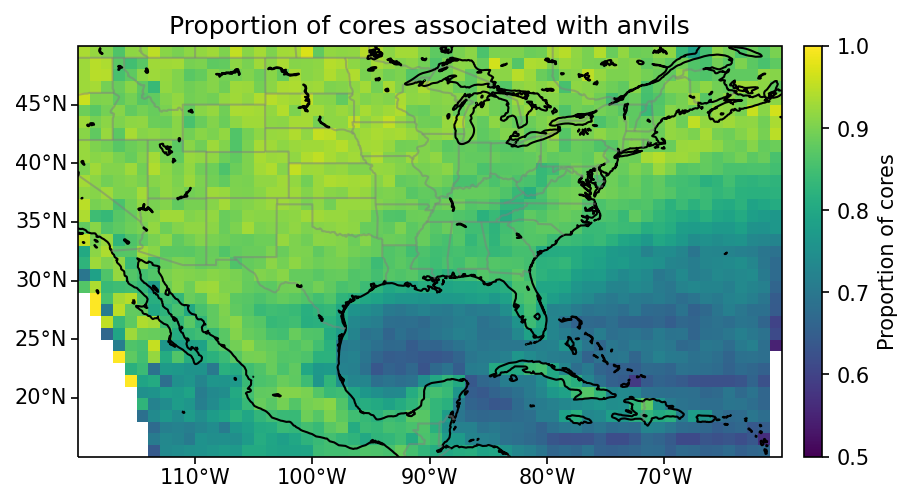
\includegraphics[width=\textwidth]{figures/ch2_04.png}
%     \caption[
%     The proportion of detection cores associated with anvils
%     ]{
%     The proportion of detection cores associated with anvils in each 1\texttimes1\textdegree\ grid box. In general, we see that the majority of cores over land are associated with anvils, while over the ocean a larger number are detected without anvils.
%     }
%     \label{fig:cores_with_anvils_map}
% \end{figure}

% Figure~\ref{fig:cores_with_anvils_map} shows the proportion of cores associated with anvil clouds.
% We see a clear land--sea contrast, with a much larger number of cores occurring without associated anvil clouds over the ocean than over land.

\subsection{Diurnal cycle of convective cores}

%f
\begin{figure}[tp]
    \centering
    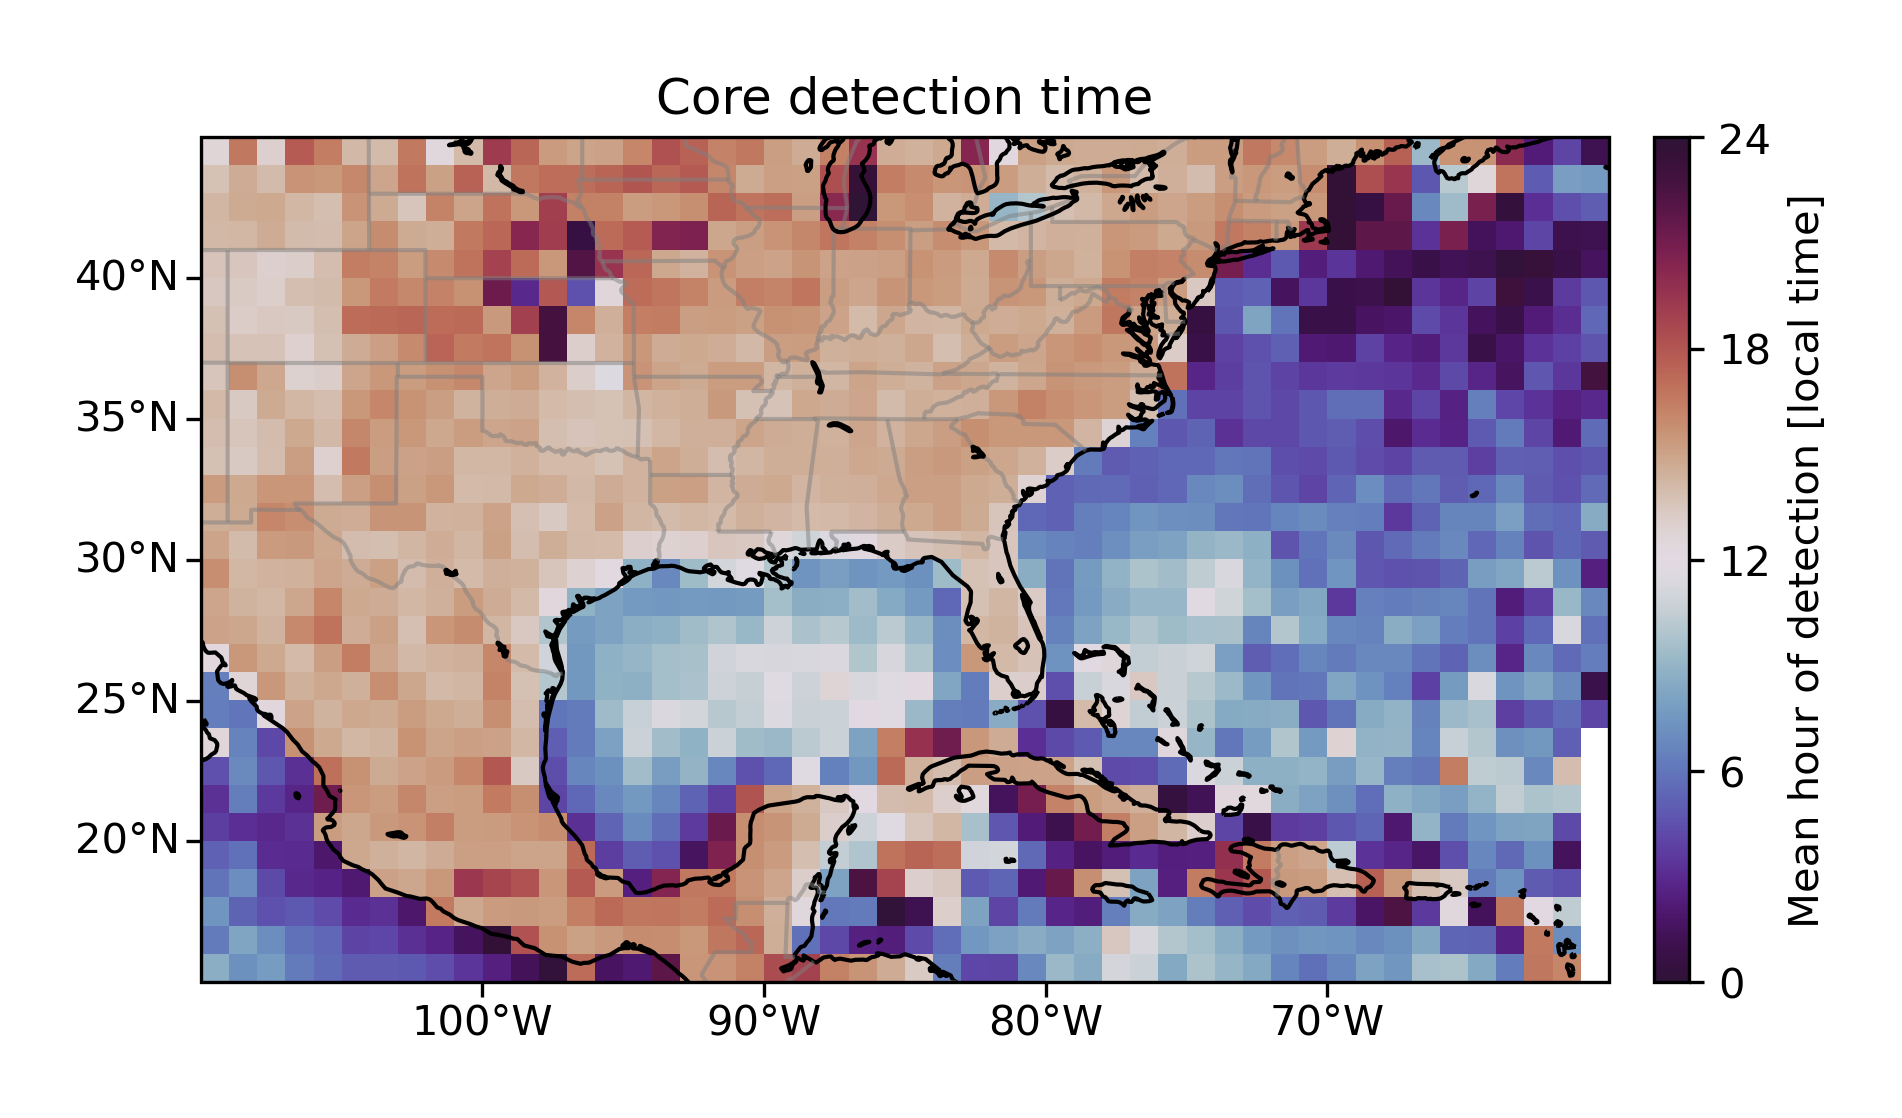
\includegraphics[width=\textwidth]{figures/chapter2_11.png}
    \caption[
    A map of average time of day of initiation of detected cores
    ]{
    The average time of day of initiation of cores observed within each 1\texttimes1\textdegree\ grid box. The time of initiation is calculated as the local solar time based on longitude, and the mean is calculated as the circular mean over a 24-hour period to account for the cyclical aspect of the hour of day.
    }
    \label{fig:core_detection_time_map}
\end{figure}

Figure~\ref{fig:core_detection_time_map}, shows the mean time of detection for cores detected within each 1-degree grid square.
The most notable feature in fig.~\ref{fig:core_detection_time_map} is the strong land-sea contrast, with the majority of land regions showing convective activity occurring during the afternoon, and the majority of ocean regions showing activity before midday.
In addition, there are a few major features of the detected time of initiation across both land and sea regions.
In coastal regions in the Gulf of Mexico and the Caribbean Sea, earlier initiation times are seen closer to coastlines, while regions further from land have average times of detection closer to midday.
Over the land there is also see a later time of initiation over the Northern Great Plains (90--100\,\textdegree W, 37--47\,\textdegree N).

% \subsubsection{Regional differences in the time of core detection}


%f
\begin{figure}[tp]
    \centering
    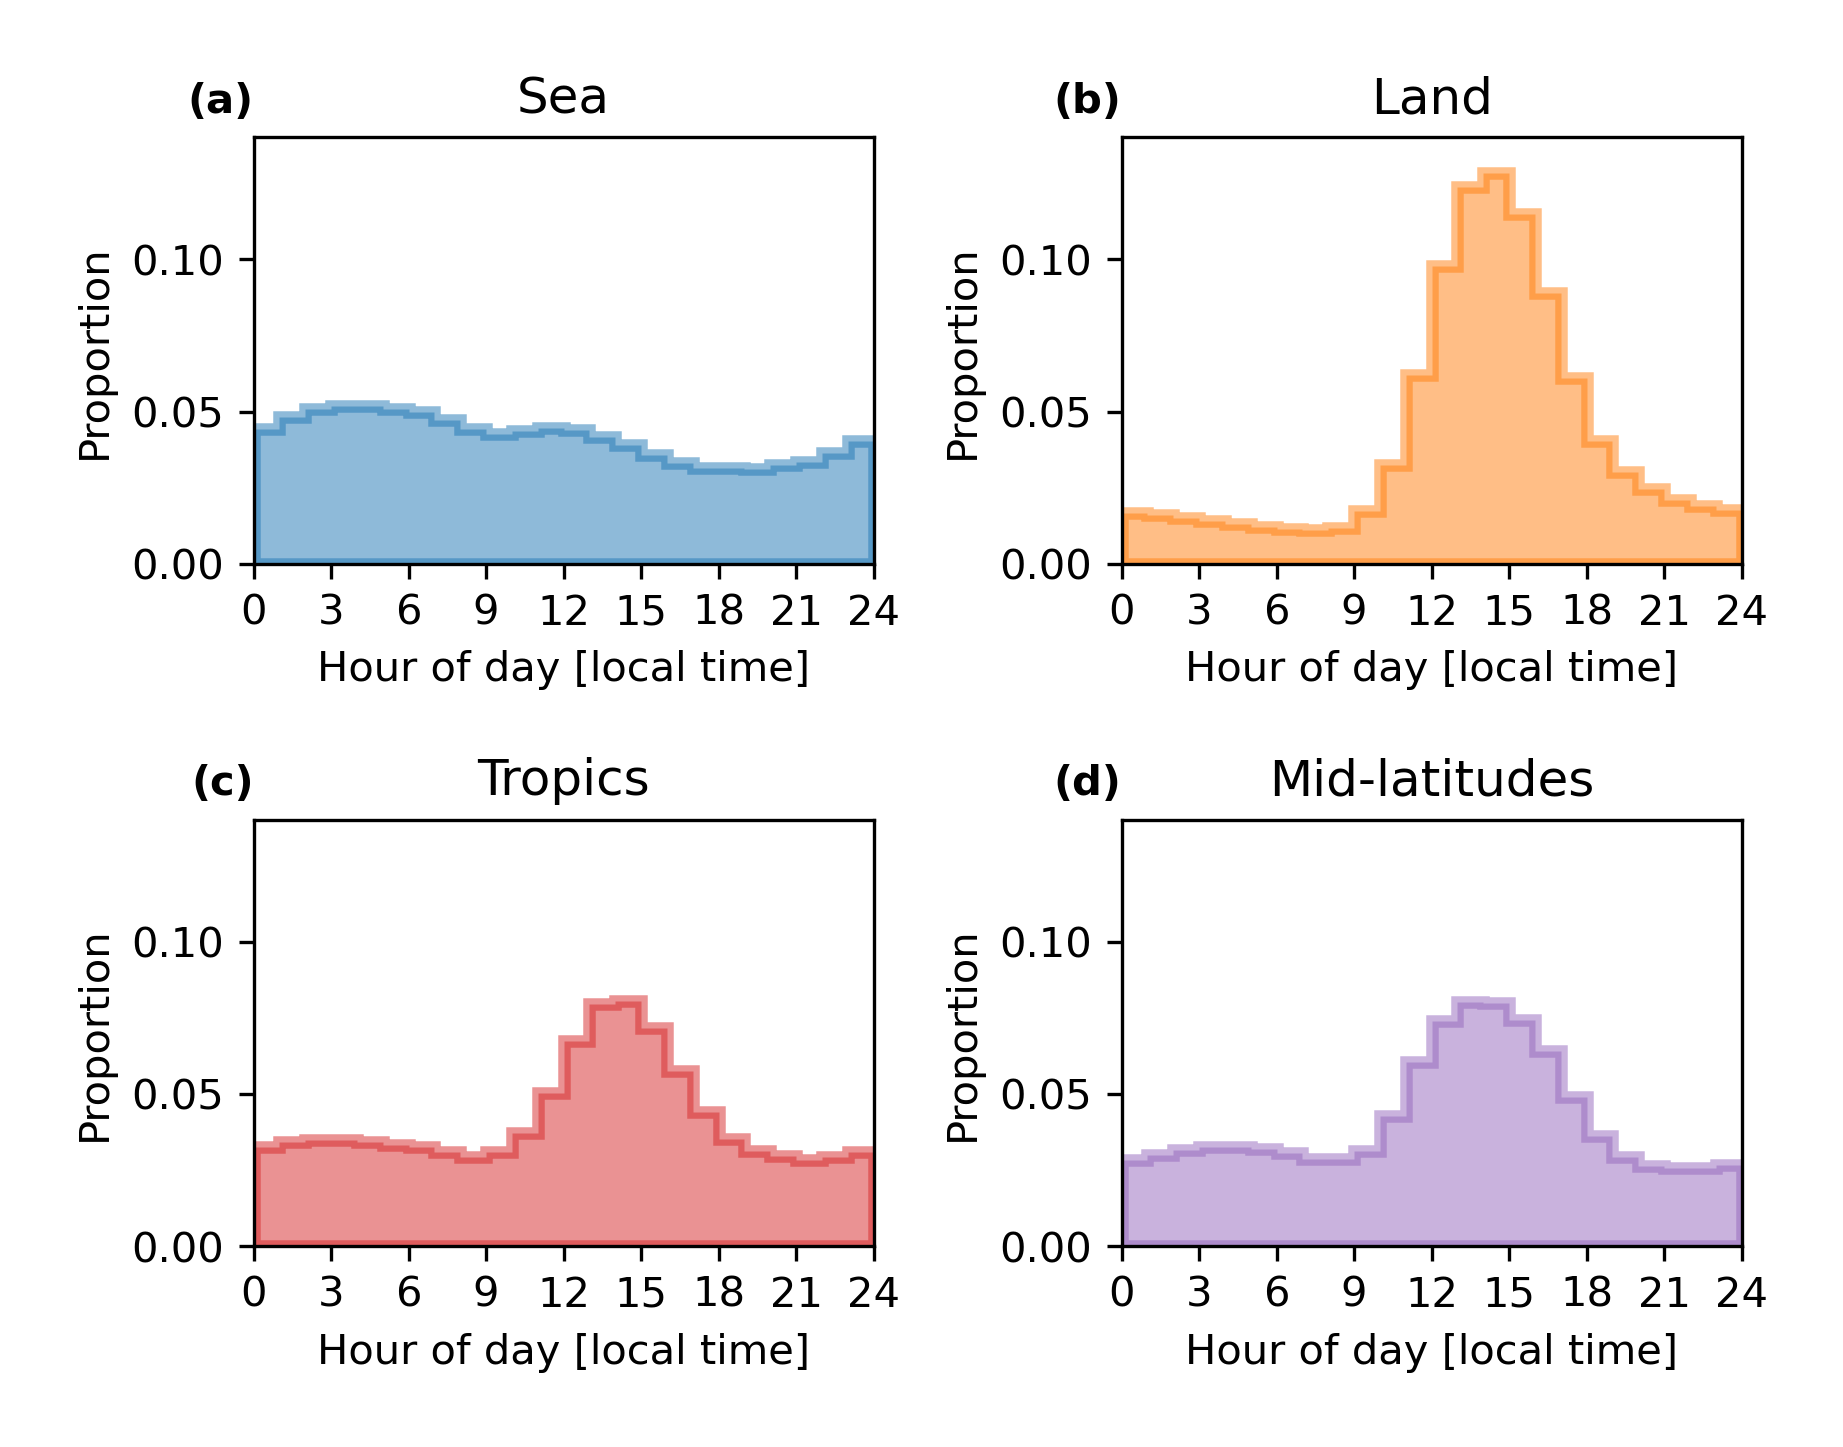
\includegraphics[width=\textwidth]{figures/chapter2_12.png}
    \caption[
    The diurnal distributions of the local time of detection for cores detected over land, sea, tropics and mid-latitudes
    ]{
    The diurnal distributions of the local time of detection for cores, binned by hour detected over (a) sea, (b) land, (c) tropics (\textless 30\,\textdegree N) and (d) mid-latitudes (\textgreater 30\,\textdegree N).
    }
    \label{fig:core_diurnal_land_sea}
\end{figure}


Figure~\ref{fig:core_diurnal_land_sea} shows the distribution of core detections across the diurnal cycle for land, sea, tropics and mid-latitude regions.
Over land there is a sharp peak in convective activity initiating in the mid-afternoon between 2 and 3 pm, with a tail extending into the night-time.
Over the sea, the distribution of core detections is much more uniform across the diurnal cycle.
There is still a peak observed in the early hours of the morning (3--6\,am), and a low in the evening (6\,pm), but the difference between these is much less pronounced than that over land.
Both the tropics and mid-latitudes have peaks in convection at the same time as that seen for all land regions in fig.~\ref{fig:core_diurnal_land_sea}\,b.
The peak for mid-latitudes is slightly broader however, with more convection occurring later in the day.

%f
\begin{figure}[tp]
    \centering
    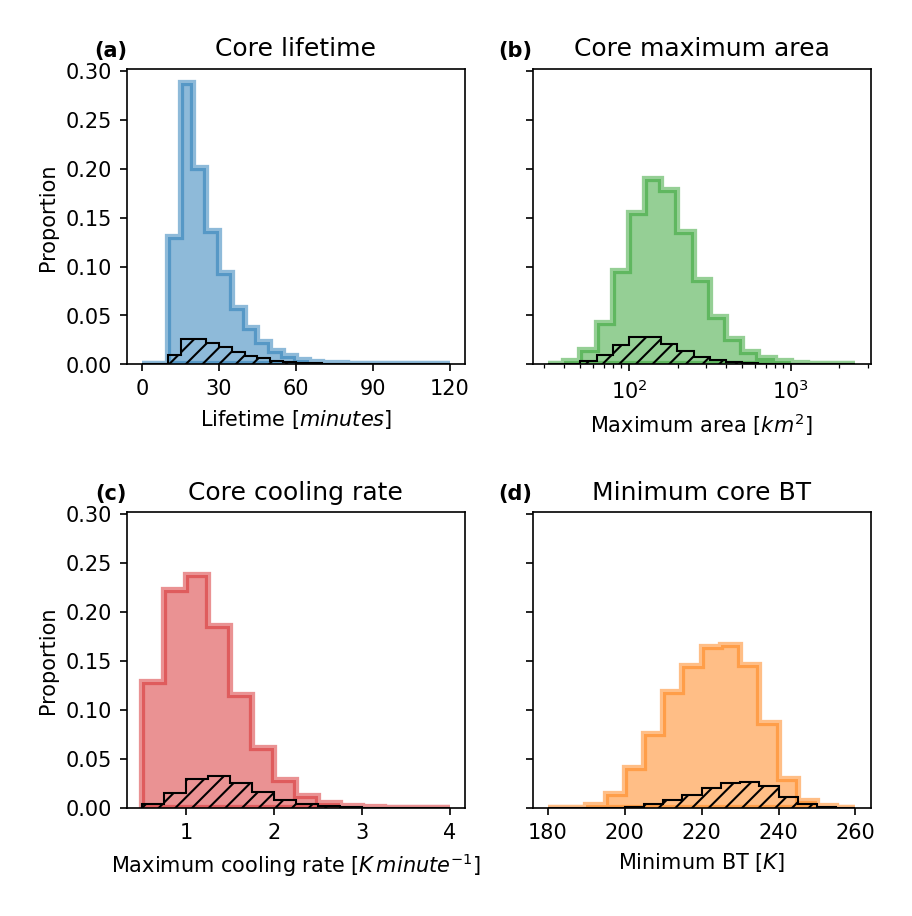
\includegraphics[width=0.75\textwidth]{figures/chapter2_13.png}
    \caption[
    The diurnal distribution of cores detected in the \acrshort{ngp} region
    ]{
    The diurnal distribution of cores detected in the \acrshort{ngp} region (37--45\,\textdegree\,N, 90--100\,\textdegree\,W).
    }
    \label{fig:core_ngp_contrast}
\end{figure}

Figure~\ref{fig:core_detection_time_map} showed a noticeably later average time of detection over the \acrfull{ngp} region.
Figure~\ref{fig:core_ngp_contrast} shows how the diurnal distribution of core detection time varies within this area, which is defined as 37--45\,\textdegree\,N, 90--100\,\textdegree\,W.
In contrast to the distribution seen over all land regions in fig.~\ref{fig:core_diurnal_land_sea}\,b, the \acrshort{ngp} region shows a later peak of convective activity between 3 and 4 pm, as well as much higher rates of convection observed during the nighttime and into the early morning until around 7\,am.
Previous studies have found a similar bimodal distribution in convective precipitation over the \acrshort{ngp} \citet{li_high-resolution_2021}.

%f
\begin{figure}[tp]
    \centering
    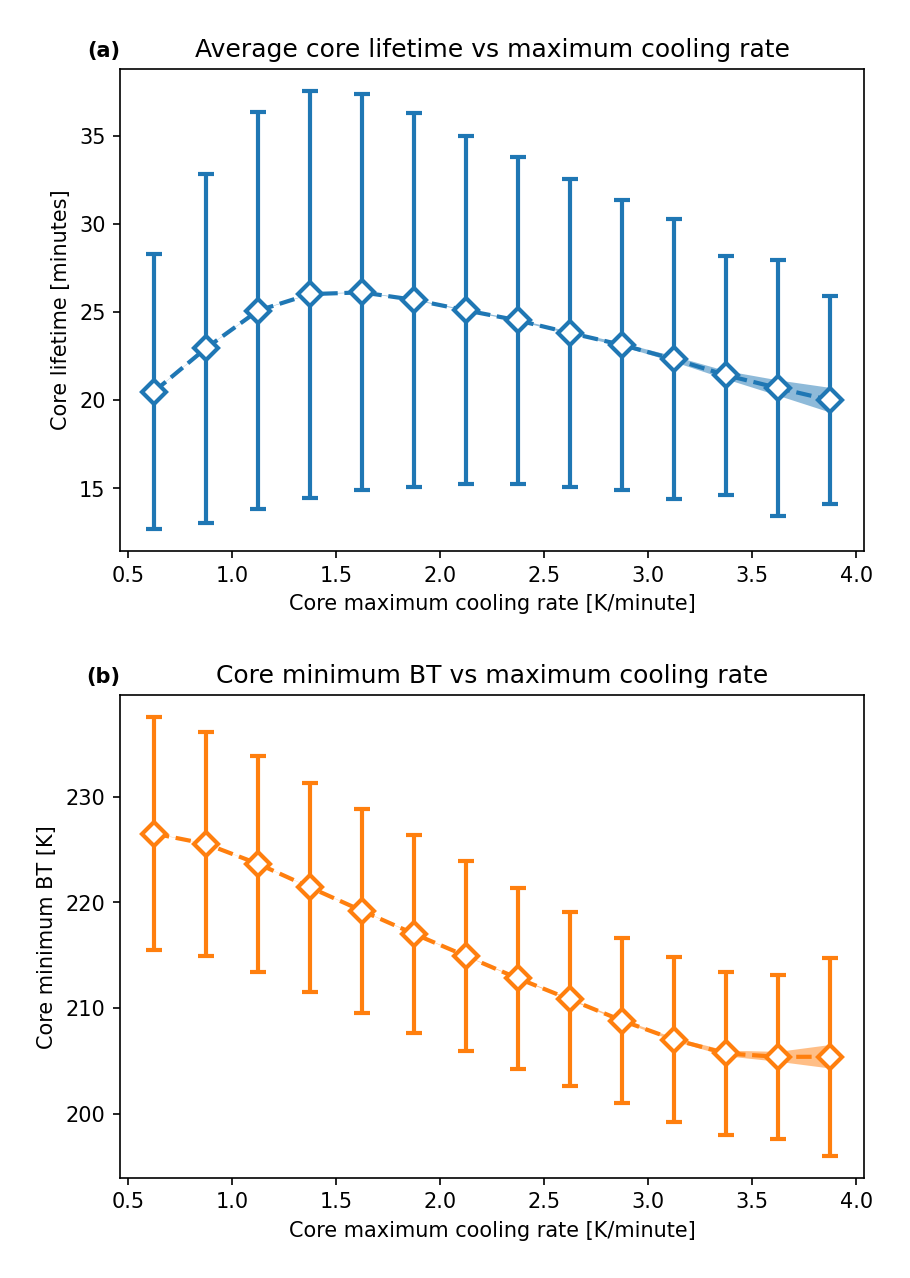
\includegraphics[width=0.75\textwidth]{figures/chapter2_14.png}
    \caption[
    The change in average time of core detection with distance from the coastline
    ]{
    The change in average time of core detection with distance from the coastline. Negative distances along the x axis show cores detected further to sea, and positive distances show cores detected further inland. Error bars show the circular standard deviation of the local solar hour of detection.
    }
    \label{fig:core_coast_effect}
\end{figure}

In fig.~\ref{fig:core_coast_effect} the effect of the distance to the coast on core detection time is examined over the Gulf Coast region (22.5--32.5\,\textdegree\,N, 82.5--100\,\textdegree\,W).
Negative distances indicate locations further offshore, and positive distances those locations further inland.
Figure~\ref{fig:core_detection_time_map} showed a change in the average time of detection of cores in locations closer to the coast, and that effect is shown again here.
For cores detected over the sea, there is a linear decrease in the average time of detection as the distance to the coast increases.
For cores detected over land, there is a sharp decrease in the time of detection very close to the coast, although further than 50\,\unit{km} from the coast this becomes a shallower linear gradient.
The linear change of core detection time with distance from the coastline may be linked to offshore and onshore breezes triggering convection.
Cores over land see a reduction in the variance of the time of detection between 50 and 150\,\unit{km} from the coast, which may also indicate that an external forcing from sea breeze is triggering convection in these areas, constraining the time of initiation of convection.

%f
\begin{figure}[tp]
    \centering
    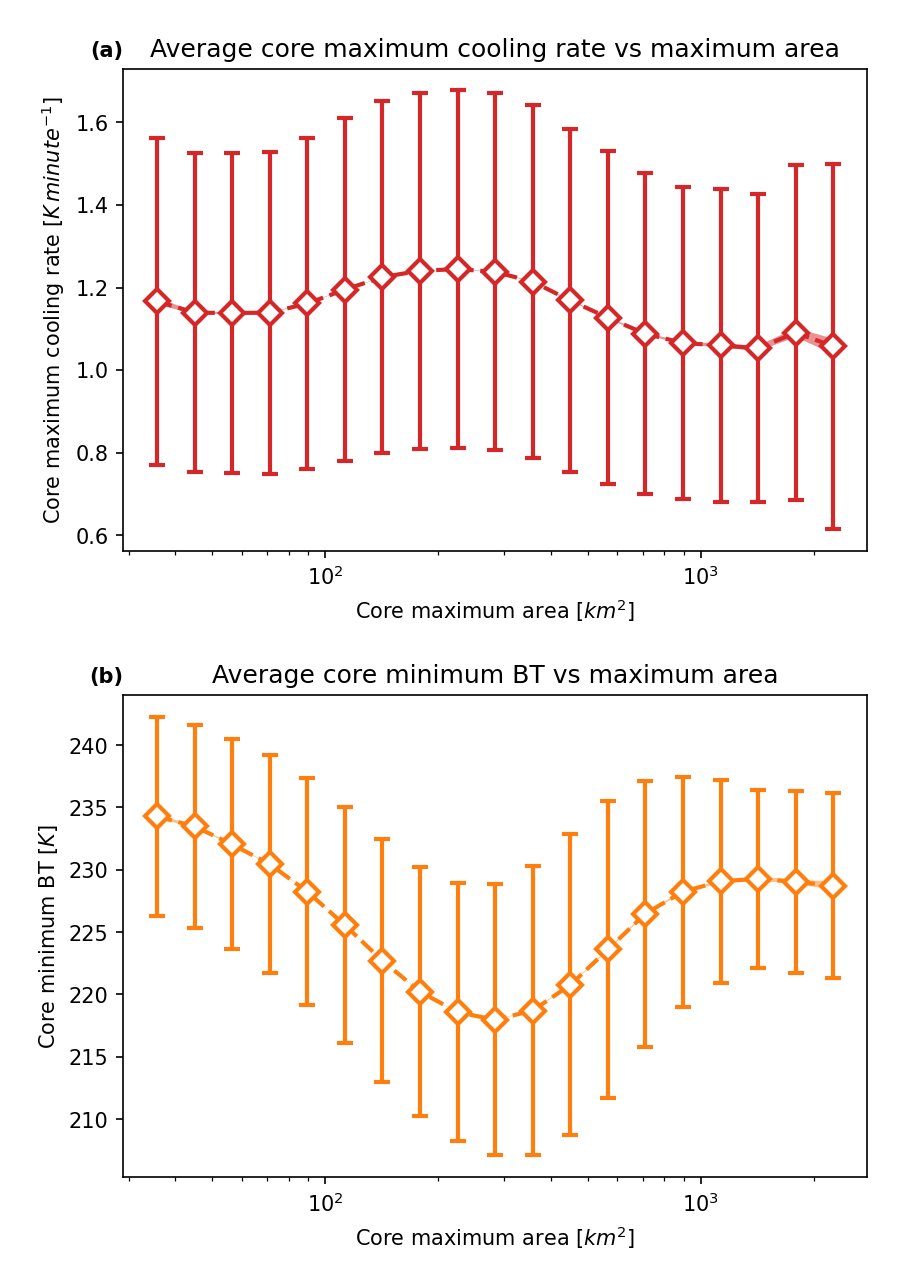
\includegraphics[width=\textwidth]{figures/chapter2_15.png}
    \caption[
    The diurnal cycle of the maximum cooling rate of cores detected over land, sea, tropics and mid-latitudes
    ]{
    The diurnal cycle of the maximum cooling rate of cores detected over (a) sea, (b) land, (c) tropics (\textless 30\,\textdegree N) and (d) mid-latitudes (\textgreater 30\,\textdegree N). Each point shows the mean of the maximum cooling rate of cores detected during that hour. Error bars show the standard deviation of maximum cooling rate.
    }
    \label{fig:core_diurnal_cooling_rate}
\end{figure}

Figure~\ref{fig:core_diurnal_land_sea} shows how the mean maximum cooling rate of cores changes across the diurnal cycle.
While over sea there is little change in cooling rate, over land there is a noticeable increase in the cooling rate throughout the daylight hours.
This leads to a peak at around 4\,pm, before cooling rate falls back to its nighttime levels which are lower than that seen over ocean.
Both tropics and mid-latitudes show similar diurnal cycles to land, albeit with a difference of 0.2\,\unit{K minute\textsuperscript{-1}} across the entire diurnal cycle.


\subsection{Distributions and properties of observed anvil clouds} \label{sec:anvil_properties}

In this section, the properties of anvil clouds in the dataset are examined.
Anvils are detected and tracked independently from cores.
Although anvils must be associated with observed cores at the start of their lifetime, tracking of anvils continues beyond the extent of the observed core lifetime.
This also allows the detection of anvils that are associated with multiple cores, providing insight into the effects of convective organisation on anvil properties.

%f
\begin{figure}[tp]
    \centering
    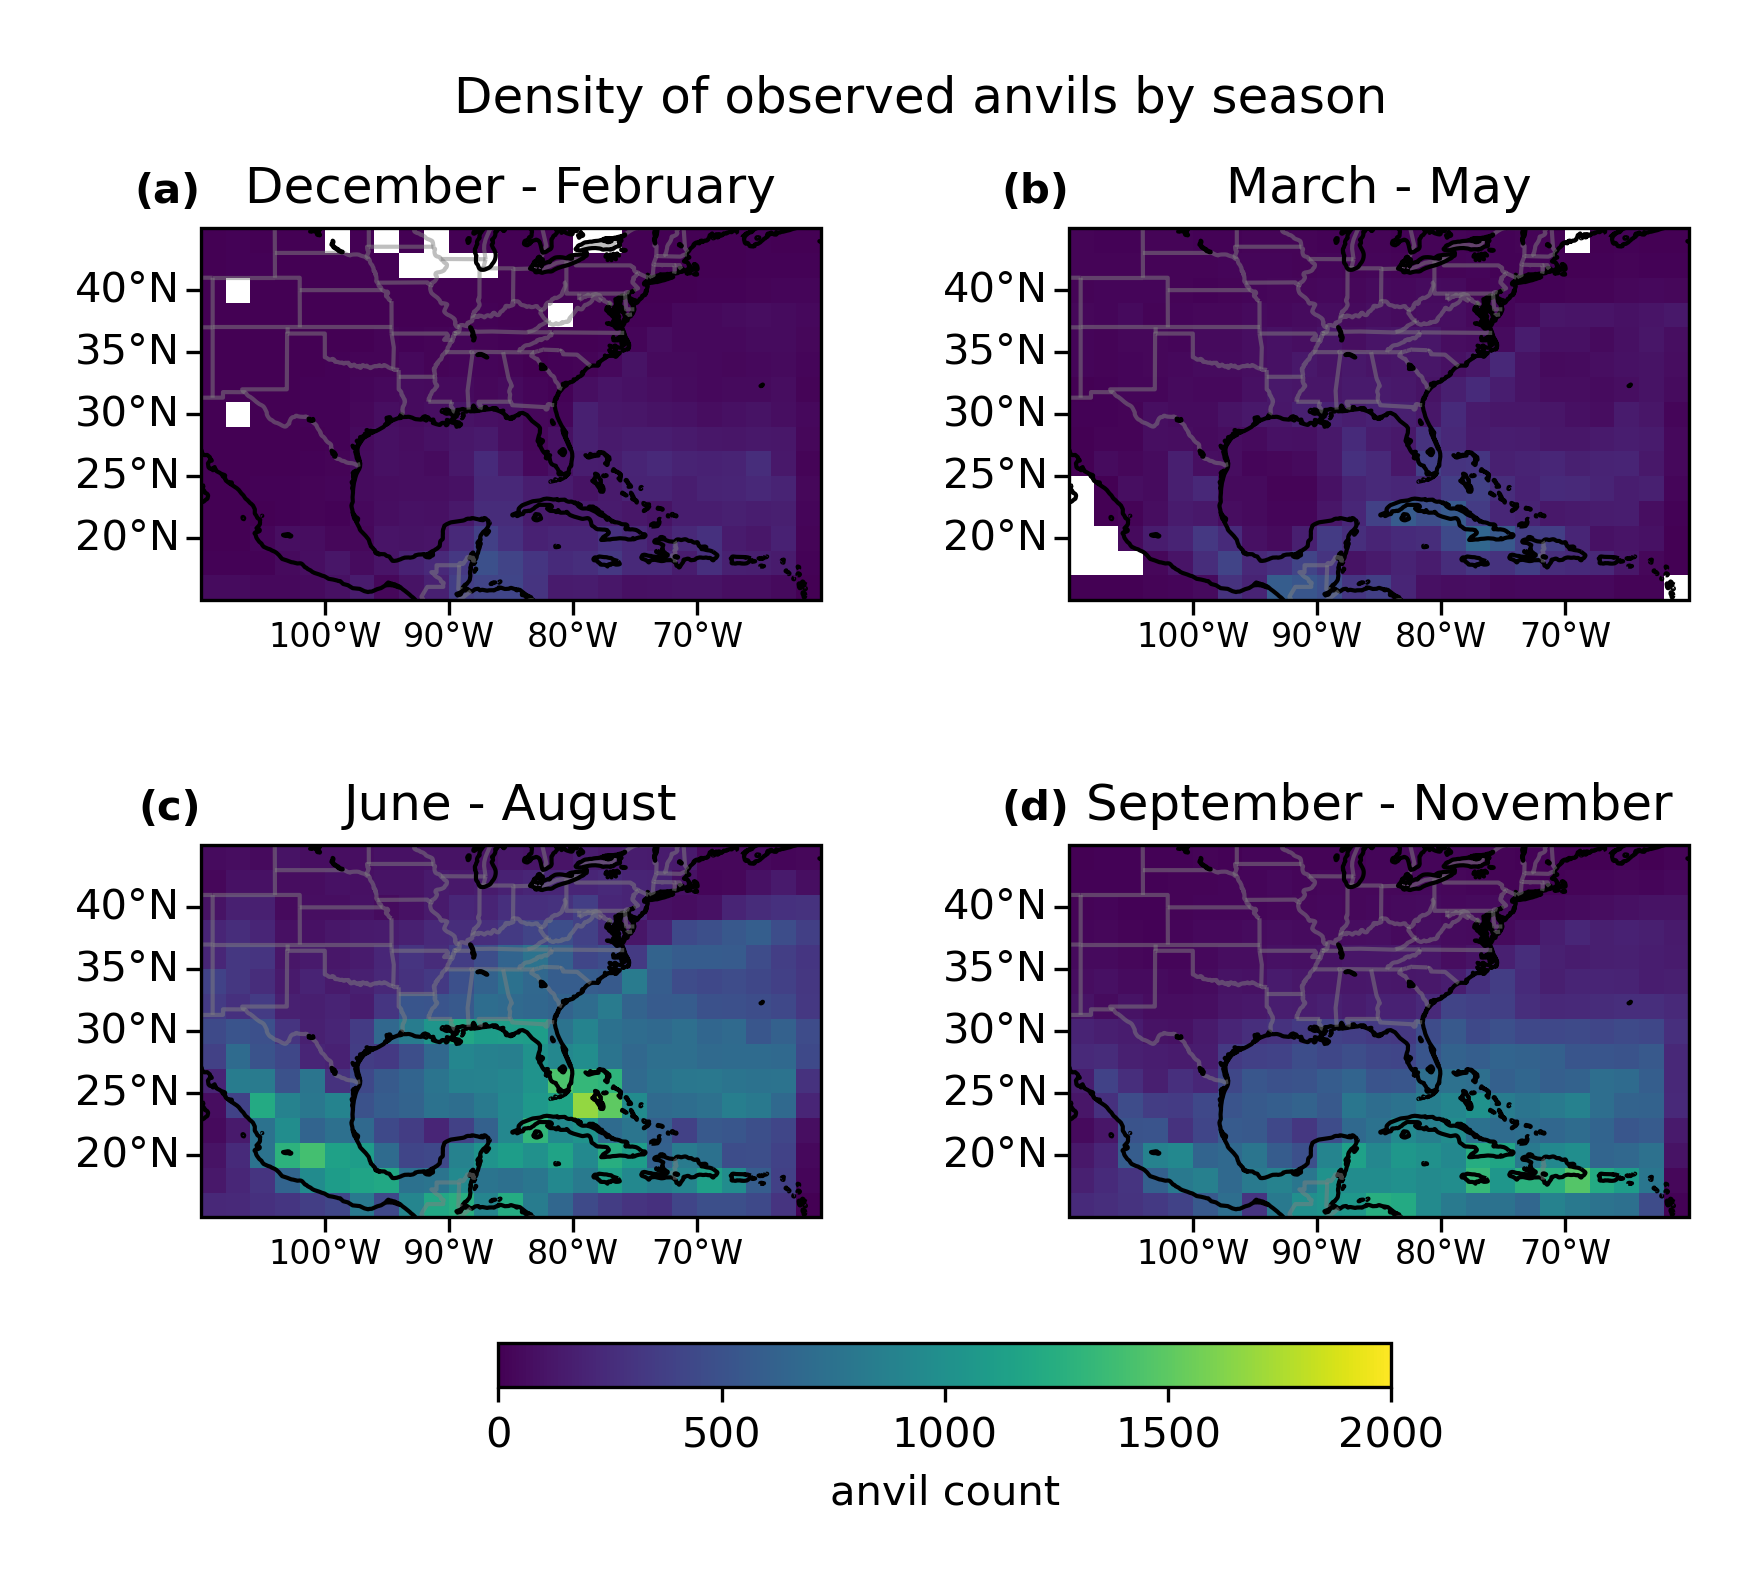
\includegraphics[width=\textwidth]{figures/chapter2_16.png}
    \caption[
    Maps showing the spatial distribution of observed anvils by season
    ]{
    Maps showing the spatial distribution of observed anvils for (a) winter, (b) spring, (c) summer and (d) autumn, each binned to a 2\texttimes2\,\textdegree grid.
    }
    \label{fig:anvil_distribution_map}
\end{figure}

Figure~\ref{fig:anvil_distribution_map} shows the counts of anvils for each 2\texttimes2\,\textdegree grid box, separated by season.
There is a similar seasonal cycle and distribution to fig.~\ref{fig:core_density_by_season}.
In winter (fig.~\ref{fig:anvil_distribution_map}\,a) and spring (fig.~\ref{fig:anvil_distribution_map}\,b) there are low rates of convection, with the majority of convection observed over warm ocean regions.
In summer, fig.~\ref{fig:anvil_distribution_map}\,c shows the highest rates of anvil detections, with a large increase in the observations of anvils over land.
In spring (fig.~\ref{fig:anvil_distribution_map}\,d), the number of anvils observed over the ocean remains high, but that over land reduces.

%f
\begin{figure}[tp]
    \centering
    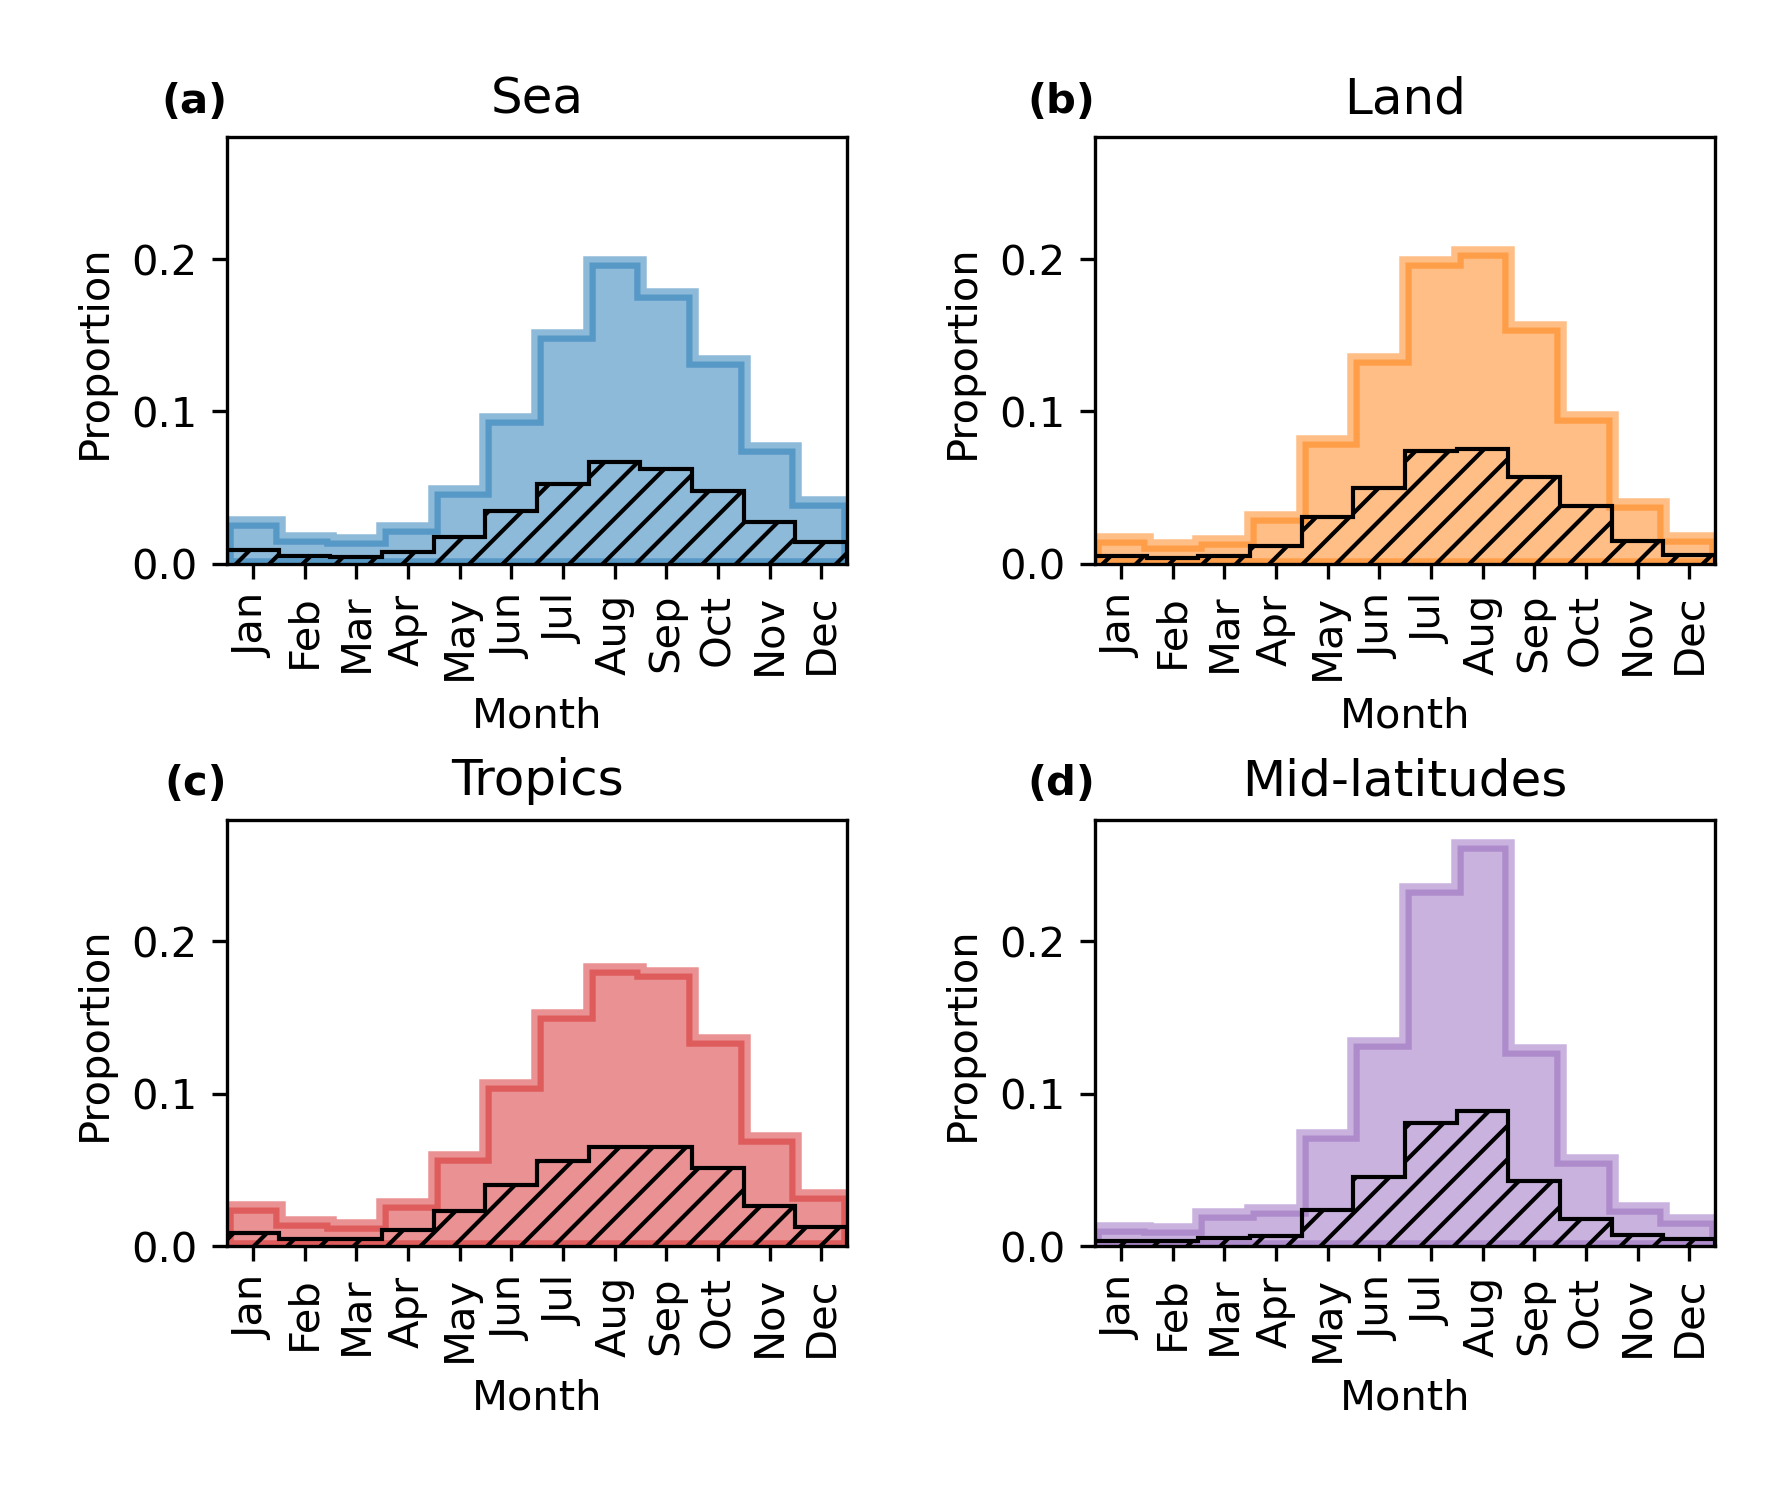
\includegraphics[width=\textwidth]{figures/chapter2_17.png}
    \caption[
    Monthly distributions of the proportion of cores detected each month over land, sea, tropics and mid-latitudes
    ]{
    Monthly distributions of the proportion of cores detected each month over (a) sea, (b) land, (c) tropics (\textless 30\,\textdegree N) and (d) mid-latitudes (\textgreater 30\,\textdegree N). The hatched area shows the proportion of the distribution consisting of anvils with multiple cores.
    }
    \label{fig:anvil_monthly_cycles}
\end{figure}

Figure~\ref{fig:anvil_monthly_cycles} shows how the annual distribution of anvil detections changes by month across different regions.
Similarly to the annual distribution of cores shown in fig.~\ref{fig:core_annual_land_sea} shows a later peak over oceans in August--September compared to July--August over land.
The mid-latitudes have a sharper peak around these two months, while the tropics show a broader distribution of anvil detections throughout the year.


%f
\begin{figure}[tp]
    \centering
    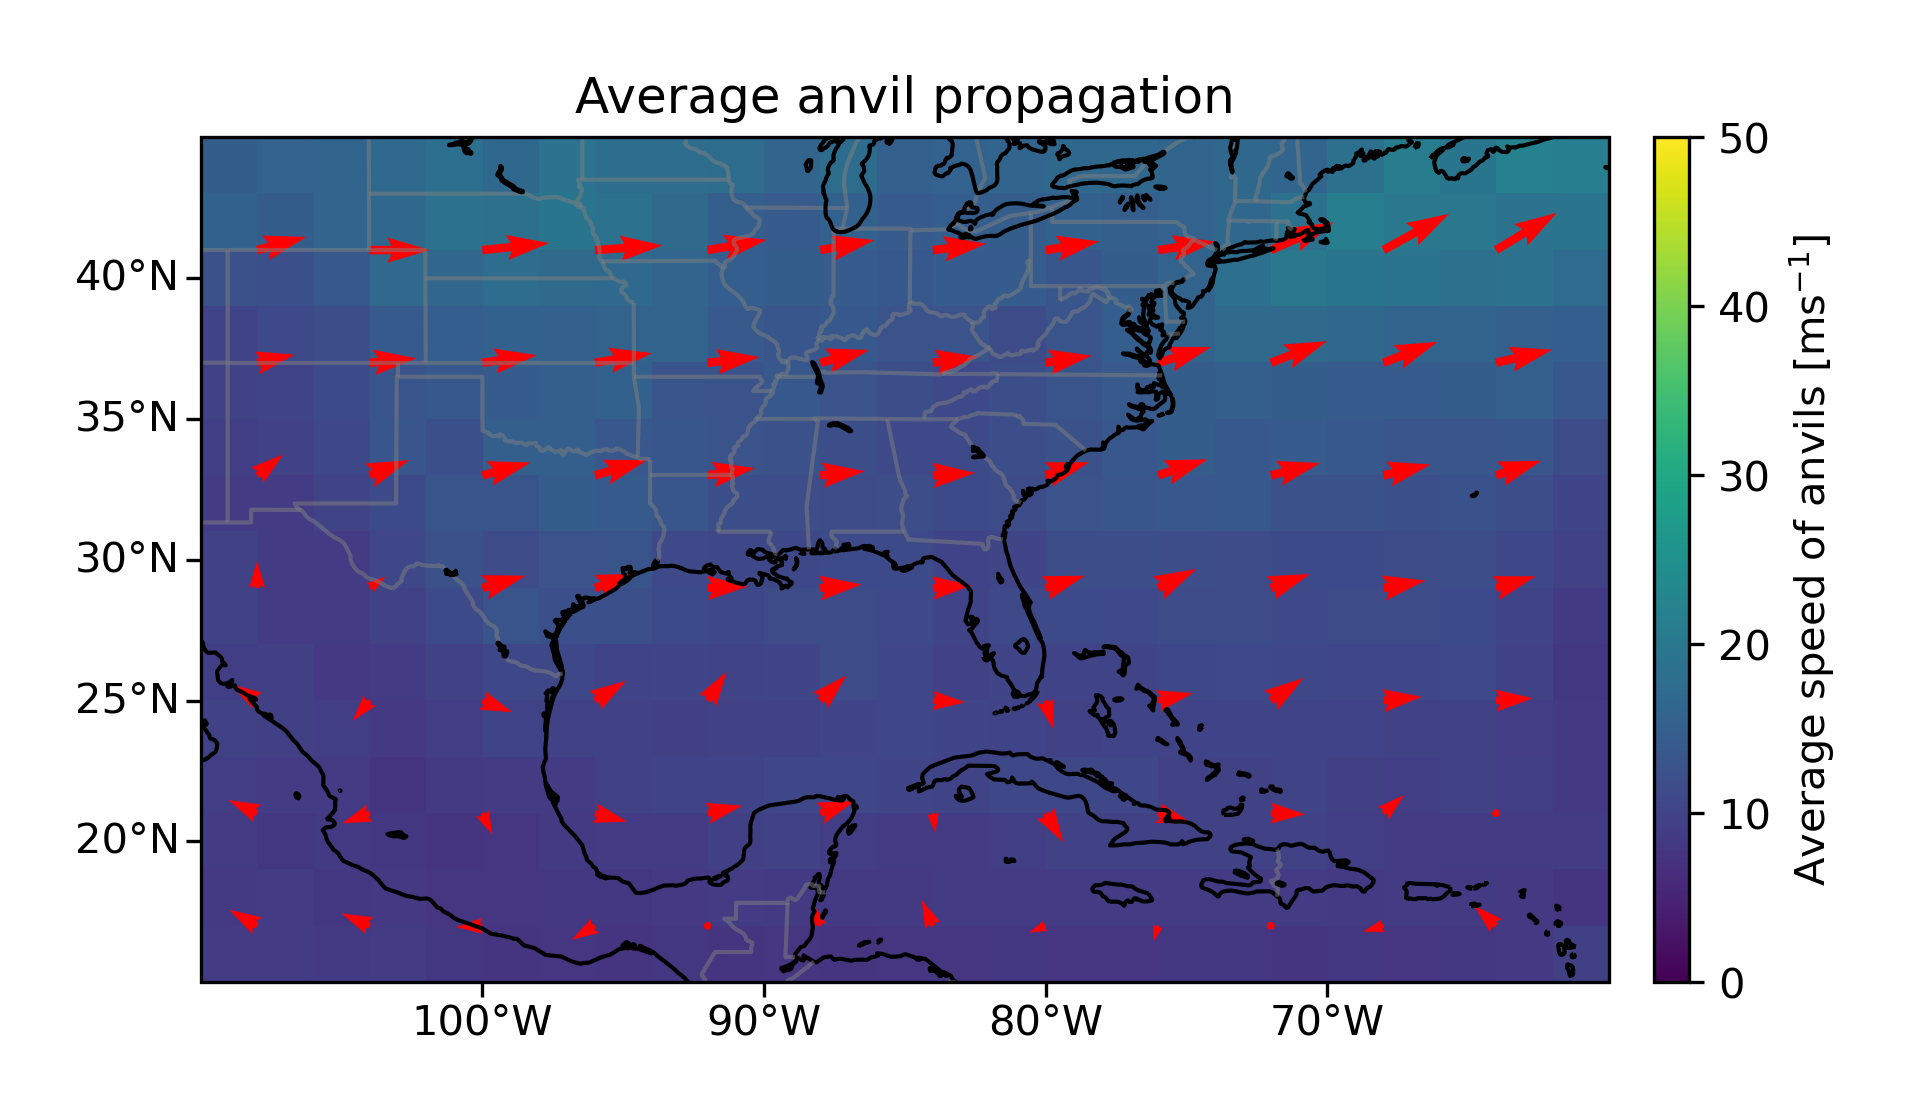
\includegraphics[width=\textwidth]{figures/chapter2_18.png}
    \caption[
    The average speed and direction of propagation of anvils
    ]{
    The average speed and direction of propagation of cores observed within each 2\texttimes2\textdegree\ grid box. The colouring shows the average speed of propagation, and the red arrows show the average direction of propagation for each 4\texttimes4\textdegree\ grid box
    }
    \label{fig:anvil_propagation_map}
\end{figure}

Figure~\ref{fig:anvil_propagation_map} shows the average propagation speed and direction for anvils in the same manner as shown for cores in fig.\ref{fig:core_propagation_map}.
In the extra-tropics (\textgreater30\,\textdegree\,N), there is generally a westerly motion, without the southerly motion seen in the cores.
This westerly motion corresponds to the prevailing high-level winds.
The change in direction and differences in the speed of propagation between anvils and cores indicates a typical shear between the two.
Over the tropics (\textless30\,\textdegree\,N) no clear overall motion of anvils is apparent.


%f
\begin{figure}[tp]
    \centering
    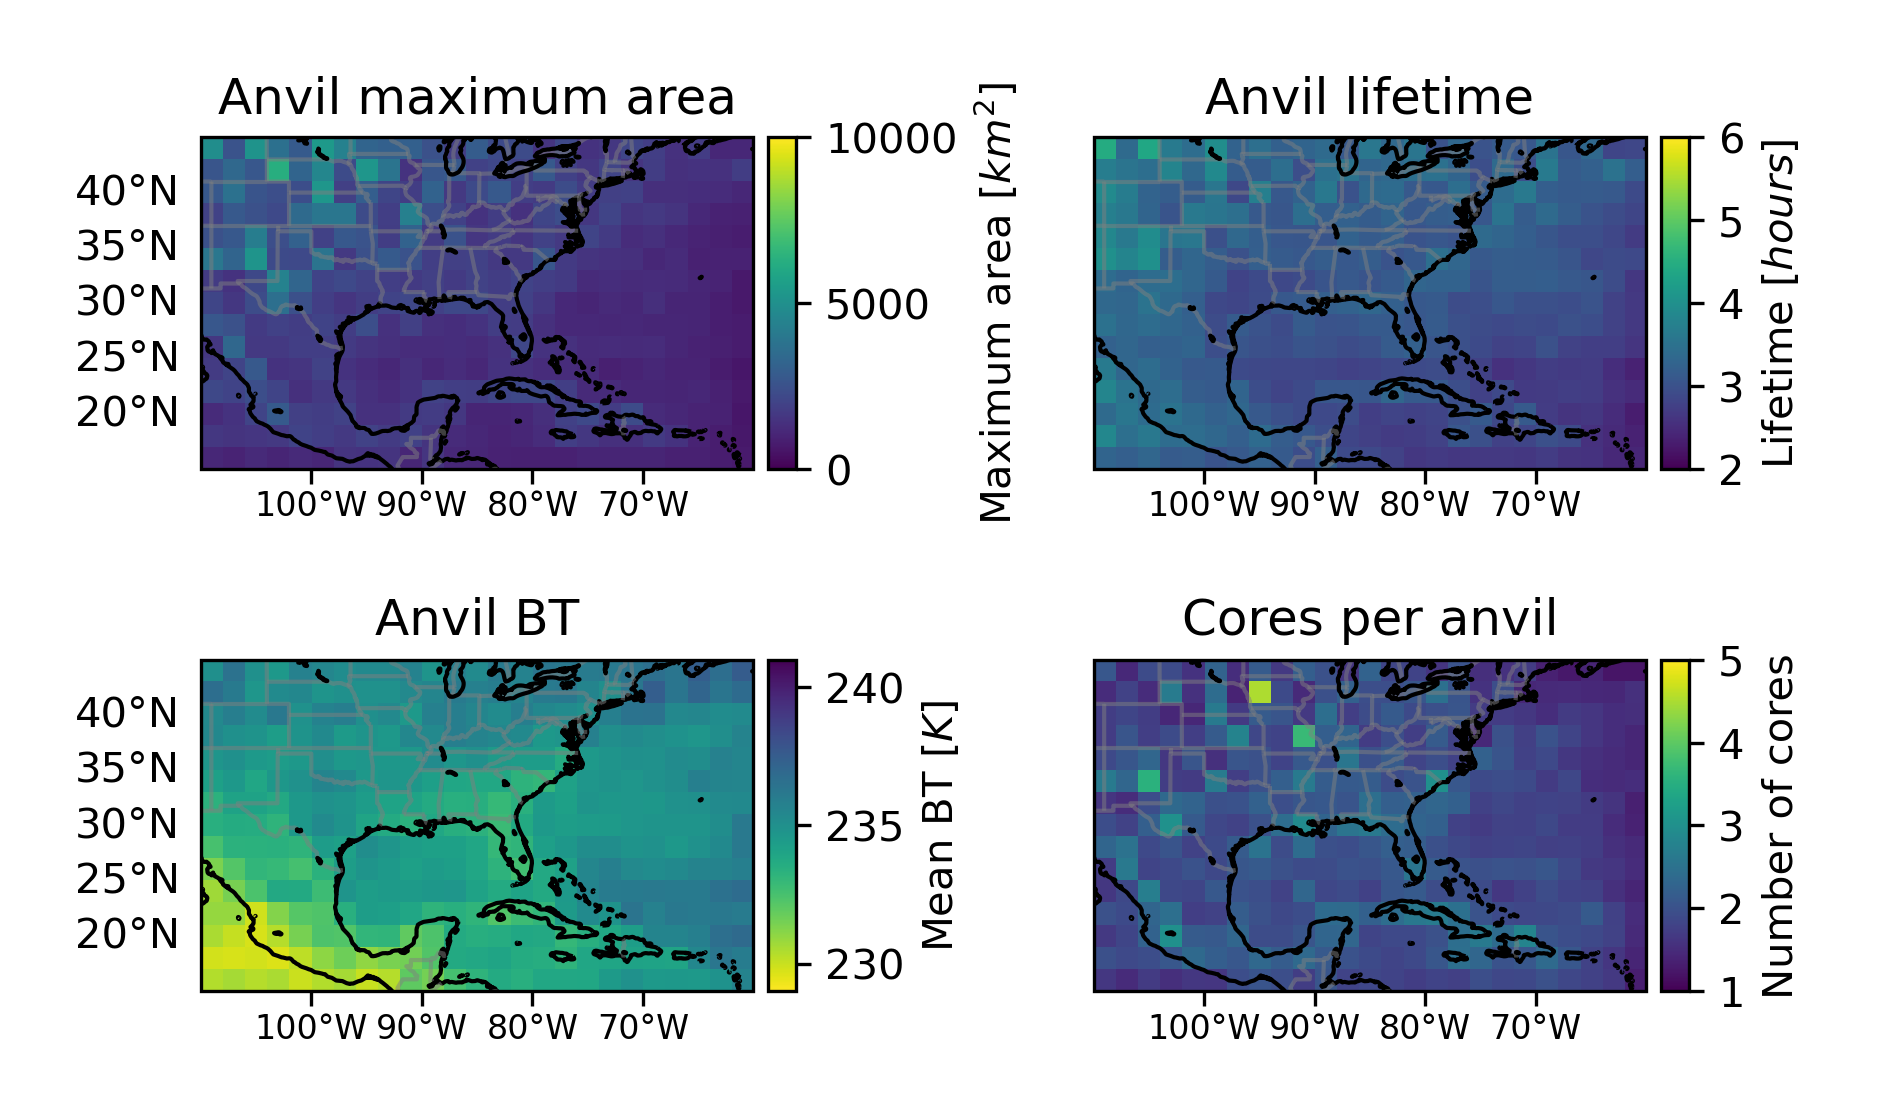
\includegraphics[width=\textwidth]{figures/chapter2_19.png}
    \caption[
    Maps showing the spatial changes in the averages of anvil maximum area, lifetime, \acrshort{bt} and number of cores
    ]{
    Maps showing the spatial changes in the averages of (a) anvil maximum area, (b) lifetime, (c) \acrshort{bt} and (d) number of cores, binned to a 2\texttimes2\,\textdegree grid.
    }
    \label{fig:anvil_properties_maps}
\end{figure}

Figure~\ref{fig:anvil_properties_maps}\,a shows the average maximum area of anvils for each 2\texttimes2\,\textdegree grid box.
There is again a land--sea contrast in the Caribbean and Gulf of Mexico.
The most notable change is the increase in anvil area towards the North--West of the domain.
This correlates with the change in sensor zenith angle---and hence the area of each pixel---shown in fig.~\ref{fig:abi_zenith_angles}.
It is possible that there is a bias towards observing larger anvils due to the larger pixel area at larger zenith angles.
However, previous studies have shown that this region is where most \acrshort{mcs}s in North America originate from \citep{feng_spatiotemporal_2019} which may also explain the large average areas.

Figure~\ref{fig:anvil_properties_maps}\,b shows the average anvil lifetime (in hours) for each 2\texttimes2\,\textdegree grid box.
There is a similar, but smaller, trend towards longer-lived anvils in the North-West of the domain as that seen for the anvil area in fig.~\ref{fig:anvil_properties_maps}\,a.
In addition, there is a tendency for average lifetimes over the ocean to be shorter than adjacent land regions.

Figure~\ref{fig:anvil_properties_maps}\,c shows the average \acrshort{bt} of anvils in each grid box.
Increasing latitude shows an increase (warming) of \acrshort{bt} over land.
In addition, there is a land--sea contrast, with warmer \acrshort{bt} over sea than land.
The coldest average \acrshort{bt} are observed over the Western coast of Mexico.

Figure~\ref{fig:anvil_properties_maps}\,d shows the average number of cores associated with each anvil in each grid box.
The Caribbean shows a noticeable land--sea contrast with an increase in the average number of cores over land, indicating that there is greater organisation of convection occurring there compared to over the sea.
For the majority of land regions the average is reasonably noisy.
This is primarily due to the presence of a small number of very large systems (including \acrshort{mcs}s), which have a very large number of cores and hence introduce noise to the spatial average.
In addition, there is see a reduction in the average number of cores towards the edge of the map which is likely due to larger anvils being more likely to be removed from the dataset by the criteria in table~\ref{table:anvil_validity_criteria}.

%f
\begin{figure}[tp]
    \centering
    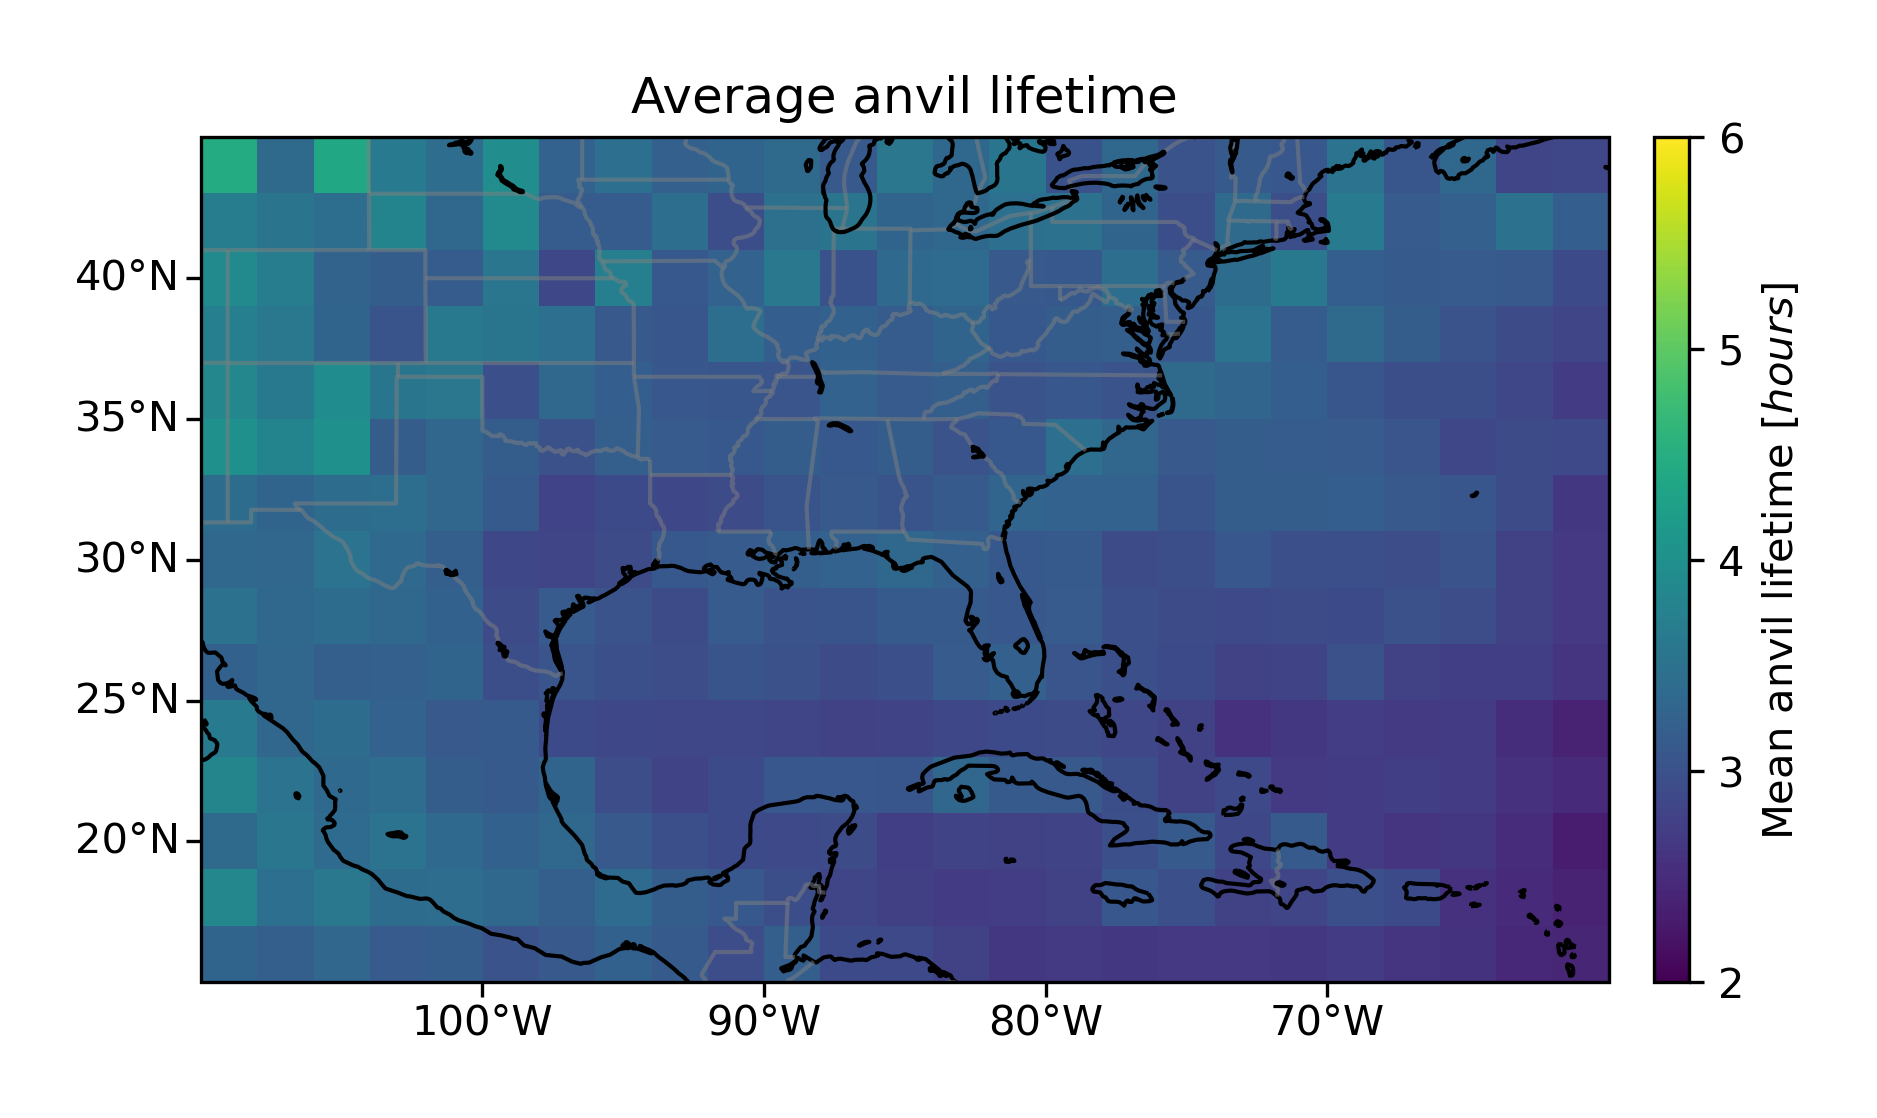
\includegraphics[width=0.9\textwidth]{figures/chapter2_20.png}
    \caption[
    Histograms showing the distribution of observed anvil properties
    ]{
    Histograms showing the distribution of observed anvil properties, with the hatched area showing the proportion associated with multiple core anvils. (a) The maximum area of the thick anvil cloud; (b) the maximum area of the thin anvil cloud (which includes both the thick and thin anvil regions; (c) the lifetime of the thick anvil and (d) the thin anvil; and (e) the average and (f) minimum observed \acrshort{bt} within each anvil.
    }
    \label{fig:anvil_properties}
\end{figure}

Figure~\ref{fig:anvil_properties} shows the distributions of anvil properties, with the proportion consisting of multiple-core anvils shown by the hatched area.
The anvil maximum area distribution has a similar shape for both thick anvils (fig.~\ref{fig:anvil_properties}\,a) and thin anvils (fig.~\ref{fig:anvil_properties}\,b), with the mean shifted to large values for the thin anvil.
It should be noted that the thin anvil area includes that of both thick and thin anvil regions, so will always be larger than that of the thick anvil alone.
The anvil lifetime distributions for the thick (fig.~\ref{fig:anvil_properties}\,c) and thin (fig.~\ref{fig:anvil_properties}\,d) anvils show a similar relationship, with a shift of the distribution to longer lifetimes for the thin anvil.
In both cases, despite the log scaling on the x-axis, there is a long tail towards larger area values and longer lifetimes.
Furthermore, this large tail consists primarily of multiple-core systems, as shown by the hatched area, indicating the impact of organisation on the area and lifetime of \acrshort{dcc}s.

Figure~\ref{fig:anvil_properties}\,e and fig.~\ref{fig:anvil_properties}\,f show the average and minimum anvil \acrshort{bt} over each detected anvil.
The minimum anvil \acrshort{bt} has a broader distribution than that of the average anvil \acrshort{bt}.
Multiple core anvils generally have colder anvil \acrshort{bt}, particularly so for the minimum \acrshort{bt}.
The cold tail of the minimum \acrshort{bt}, with values less than 200\,\unit{K}, indicates the presence of overshooting tops within these organised systems.

%f
\begin{figure}[tp]
    \centering
    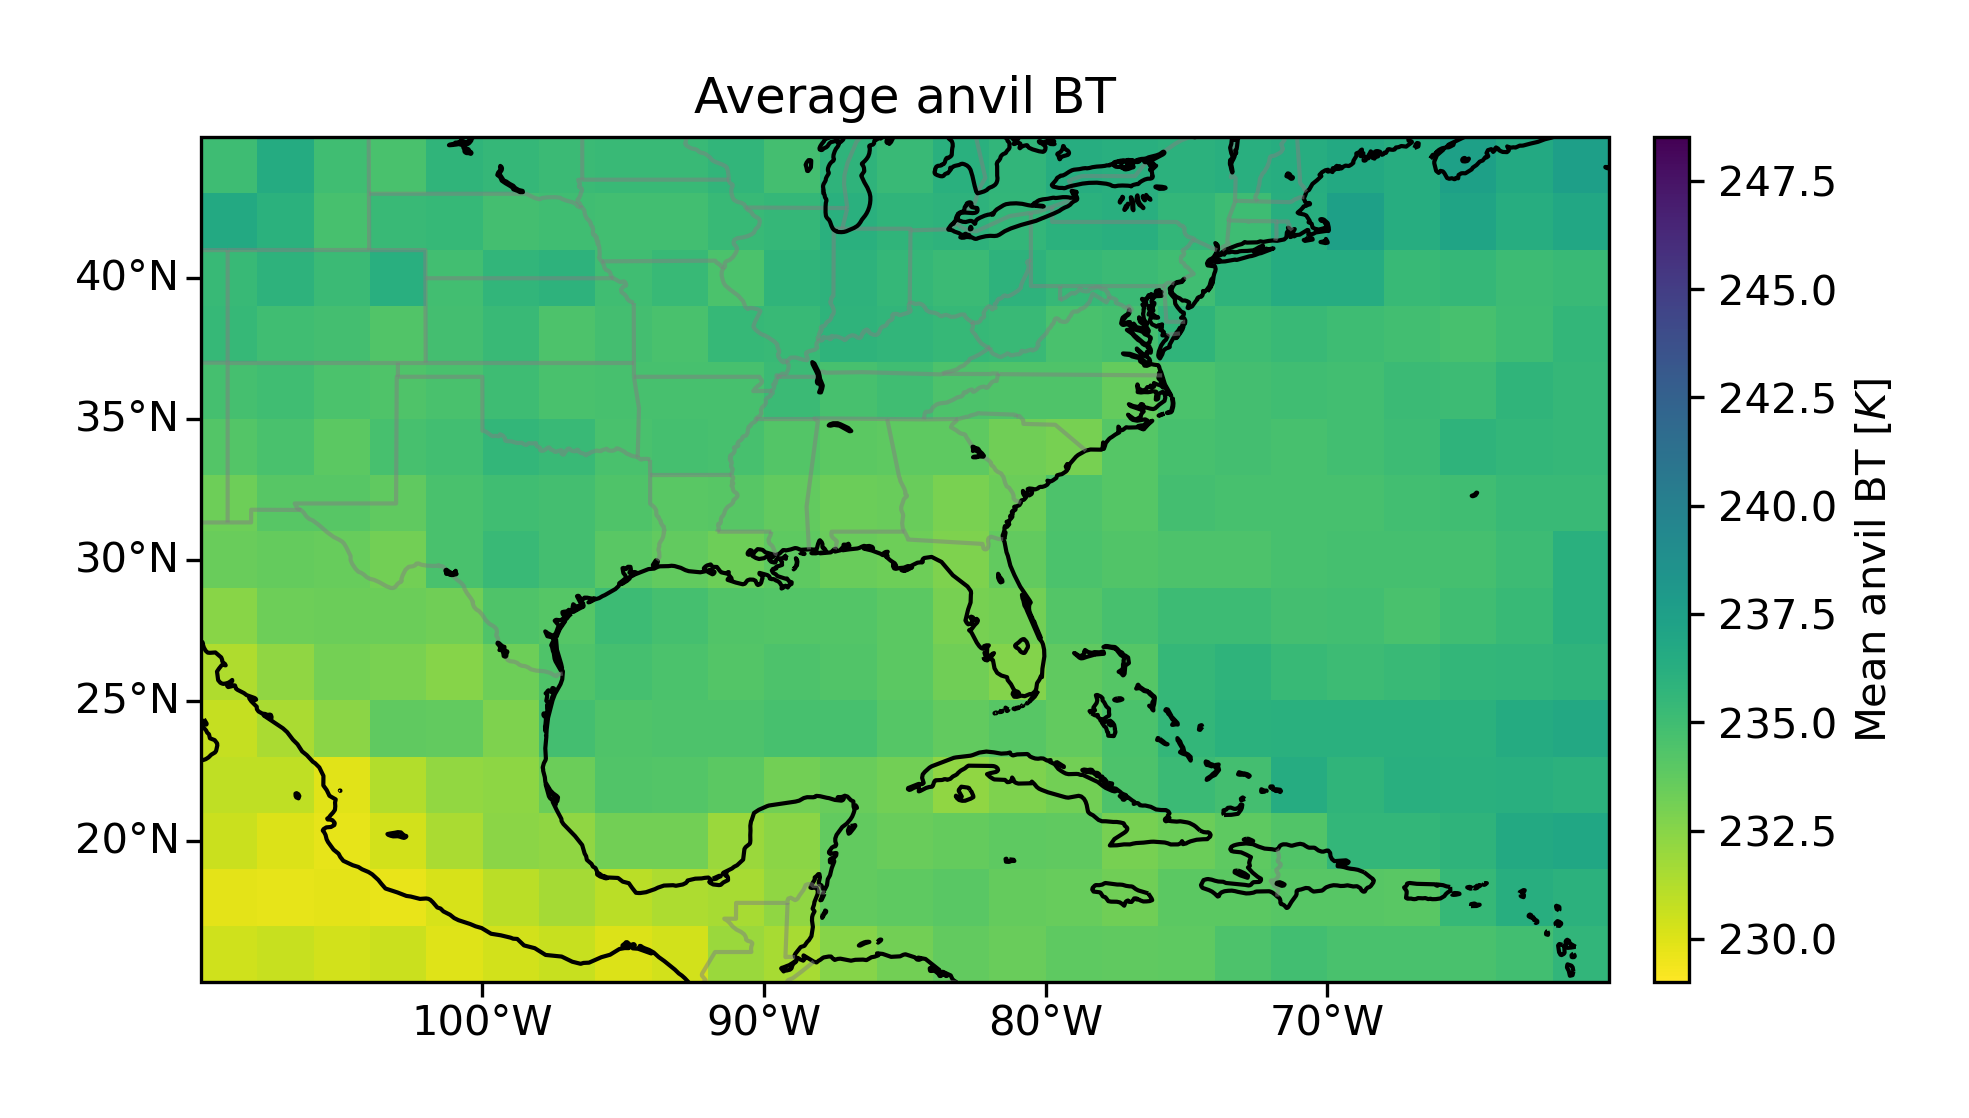
\includegraphics[width=0.9\textwidth]{figures/chapter2_21.png}
    \caption[
    The change in the average area and lifetime of anvils with different number of cores, and their total area coverage.
    ]{
    The change in the average area and lifetime of anvils with different number of cores. Mean values of (a) maximum thick anvil area, (b) maximum thin anvil area, (c) thick anvil lifetime and (d) thin anvil lifetime all increase with increasing number of cores. (e) The proportion of all anvils with different numbers of cores and (f) the fraction of total anvil coverage attributed to those anvils.}
    \label{fig:anvil_cores_and_coverage}
\end{figure}

Figure~\ref{fig:anvil_cores_and_coverage}\,a, b, c and d the average of the thick anvil maximum area, thin anvil maximum area, thick anvil lifetime and thin anvil lifetime for anvils with different numbers of cores.
In all cases these areas and lifetimes increase with an increasing number of cores.
In particular, the increase in the number of cores has a large impact on the maximum area of anvils, 
The most organised systems, which contain 10 or more cores, have areas that are more than two orders of magnitude greater on average than the anvils of isolated \acrshort{dcc}s.

Figure~\ref{fig:anvil_cores_and_coverage}\,e and f show the distribution of the number of cores associated with each detected anvil, and the proportion of total anvil coverage attributed to anvils with different core counts respectively.
Overall, the vast majority of anvils detected are isolated \acrshort{dcc}s with only a single core.
For anvils with greater than five cores, the number of systems observed drops to such a level that grouping of these \acrshort{dcc}s into bins of 6--9 cores and 10 or more is performed to ensure that there is a representative sample size of each group.
Despite making up the majority of observed \acrshort{dcc}s, single core systems only make up 12\% of the total anvil coverage.
Instead, despite being few in number, it is the most organised \acrshort{dcc}s---those with ten or more cores---which are responsible for the majority of anvil coverage due to their large area and lifetime.
The large area and lifetime of these systems---seen in the long tails of those distributions in fig.~\ref{fig:anvil_properties}---compound to result in this large coverage.

%f
\begin{figure}[tp]
    \centering
    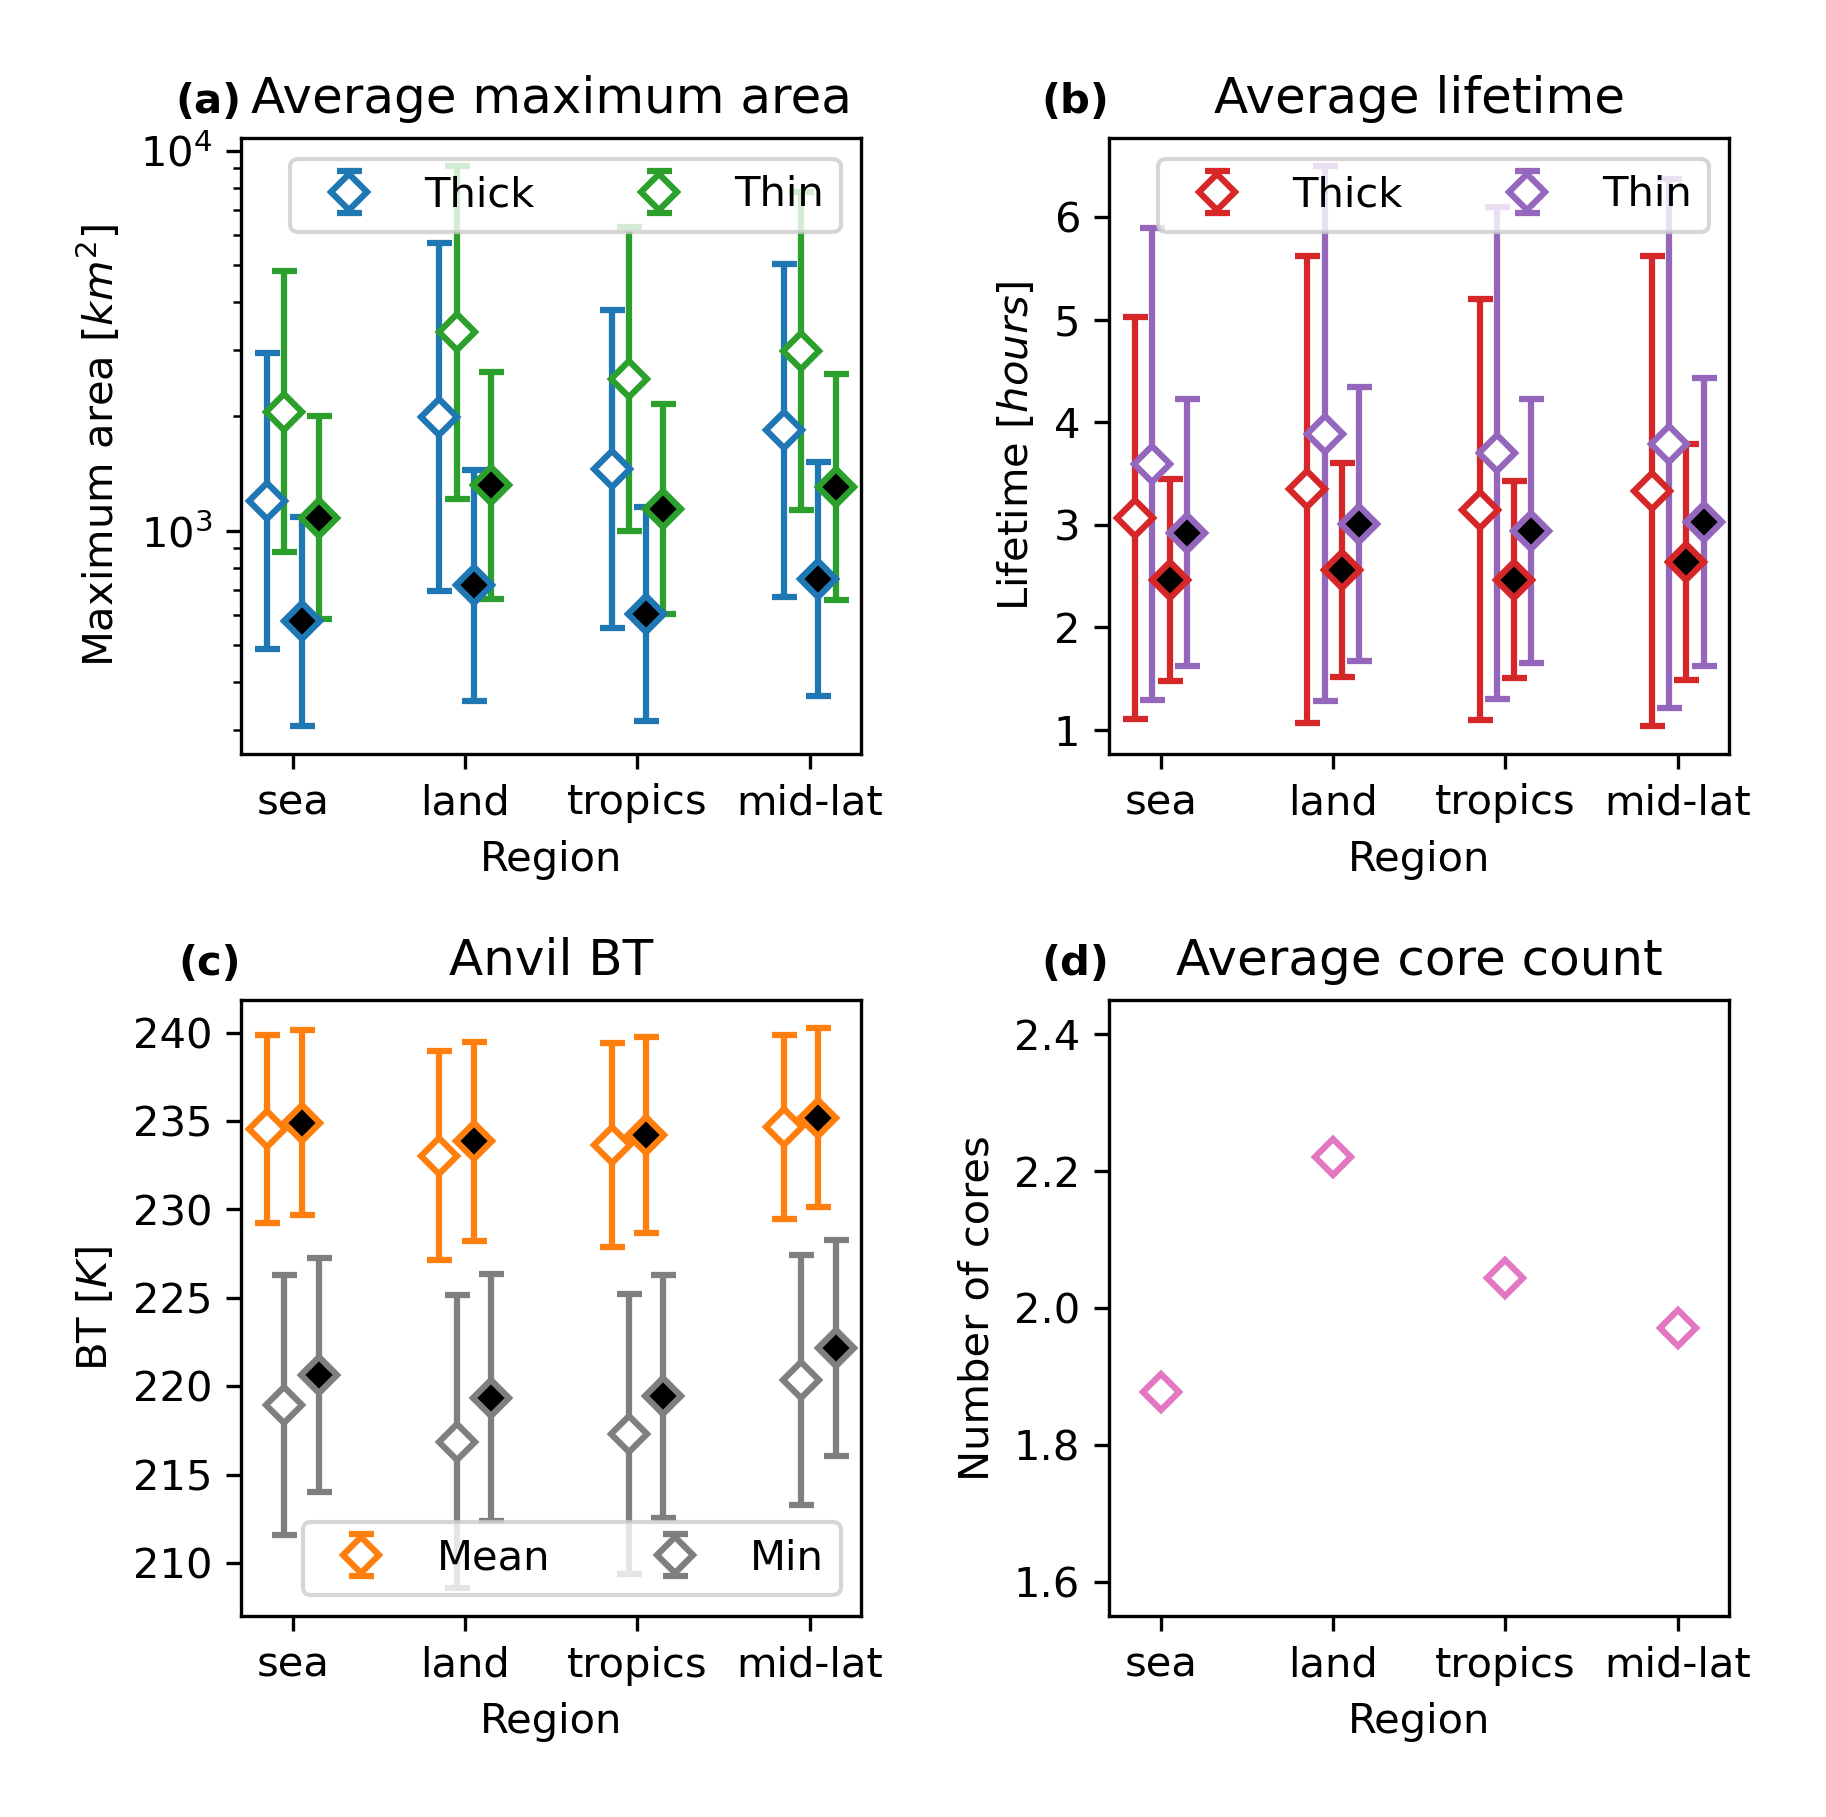
\includegraphics[width=0.9\textwidth]{figures/chapter2_22.png}
    \caption[
    The change in the average areas, lifetimes, \acrshort{bt} and number of cores of anvils observed over sea, land, tropics and mid-latitudes.
    ]{
    The change in the average (a) areas, (b) lifetimes, (c) \acrshort{bt} and (d) number of cores of anvils observed over sea, land, tropics and mid-latitudes. The points with no fill show the average across all \acrshort{dcc}s, whereas the points with the black fill show the average for isolated \acrshort{dcc}s (with one core) only. Error bars show the standard deviation on the mean.
    }
    \label{fig:anvil_properties_regions}
\end{figure}

Figure~\ref{fig:anvil_properties_regions} shows how the averages of the maximum areas, lifetimes, \acrshort{bt} and number of cores vary between different regions.
For both isolated and multi-core convection, the average areas and lifetimes shown in fig.~\ref{fig:anvil_properties_regions}\,a and b respectively are larger over land than sea, and in the mid-latitudes than in the tropics.
For the anvil \acrshort{bt} shown in fig.~\ref{fig:anvil_properties_regions}\,c, both the mean and minimum \acrshort{bt} of anvils is colder over land than sea, and also colder in the tropics than in the mid-latitudes.
\acrshort{dcc}s over land tend to have more cores than those over sea, however is is clear that as these differences also apply to isolated \acrshort{dcc}s, they are connected to changes in the convective processes and anvil evolution in the different regions, rather than simply a sampling bias.

\subsection{Diurnal cycle of anvils}

%f
\begin{figure}[tp]
    \centering
    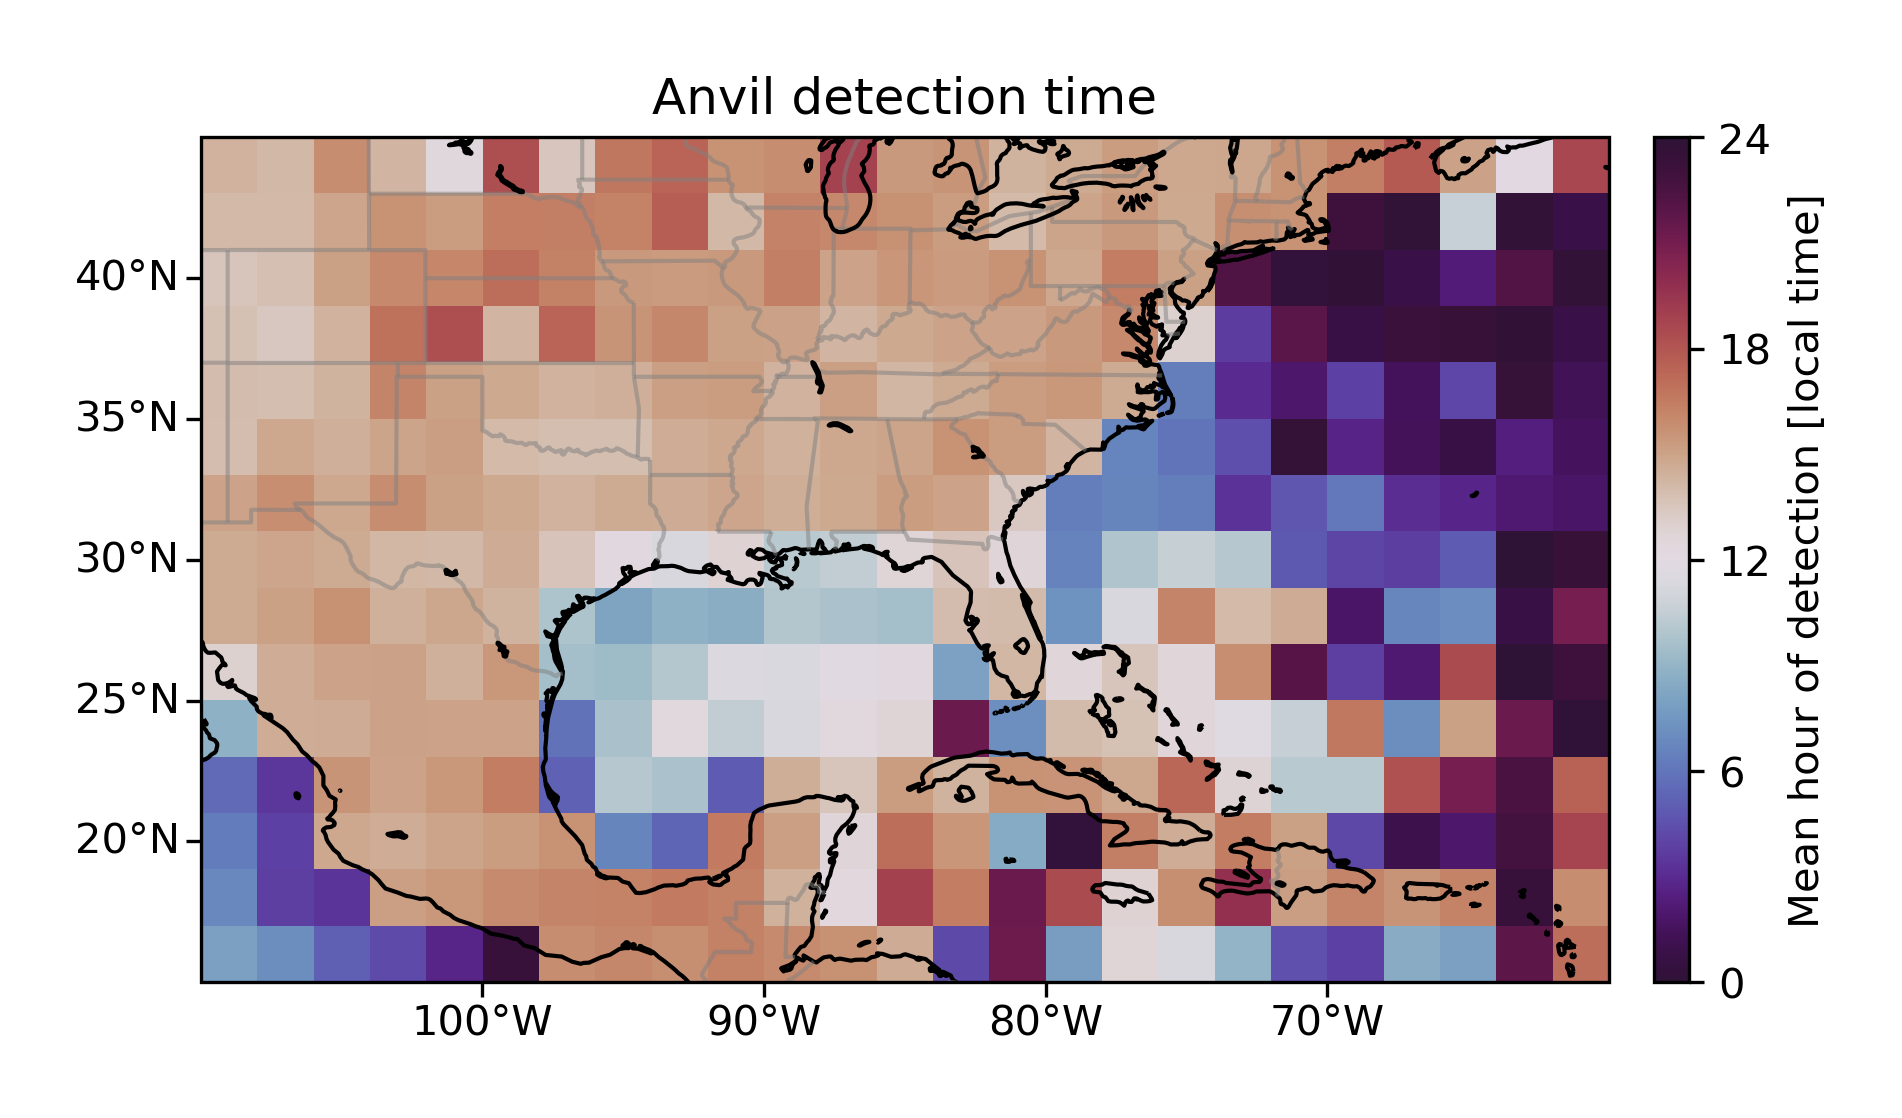
\includegraphics[width=\textwidth]{figures/chapter2_23.png}
    \caption[
    The average time of detection of anvils
    ]{
    The average time of day of detection of anvils observed within each 2\texttimes2\textdegree\ grid box, calculated as the circular mean of the local solar time.
    }
    \label{fig:anvil_detection_time_map}
\end{figure}

Figure~\ref{fig:anvil_detection_time_map} shows the average local time of day of anvil detection.
Similar to fig.~\ref{fig:core_detection_time_map} a strong land--sea contrast is seen.
However, over parts of the Caribbean Sea the average time of anvil detection is in the afternoon rather than in the morning, which may be linked to anvils that initiate over land but are advected over the ocean.
There is also a later average time of detection of anvils over the \acrshort{ngp} region, although this shows less of a contrast with surrounding land regions than that of the core initiation times.
This indicates that the second peak of core convective activity during the nighttime and early morning in fig.~\ref{fig:core_ngp_contrast} is linked to long-lived, multiple core systems including \acrshort{mcs}s, similar to what was found by \citet{feng_spatiotemporal_2019}.

%f
\begin{figure}[tp]
    \centering
    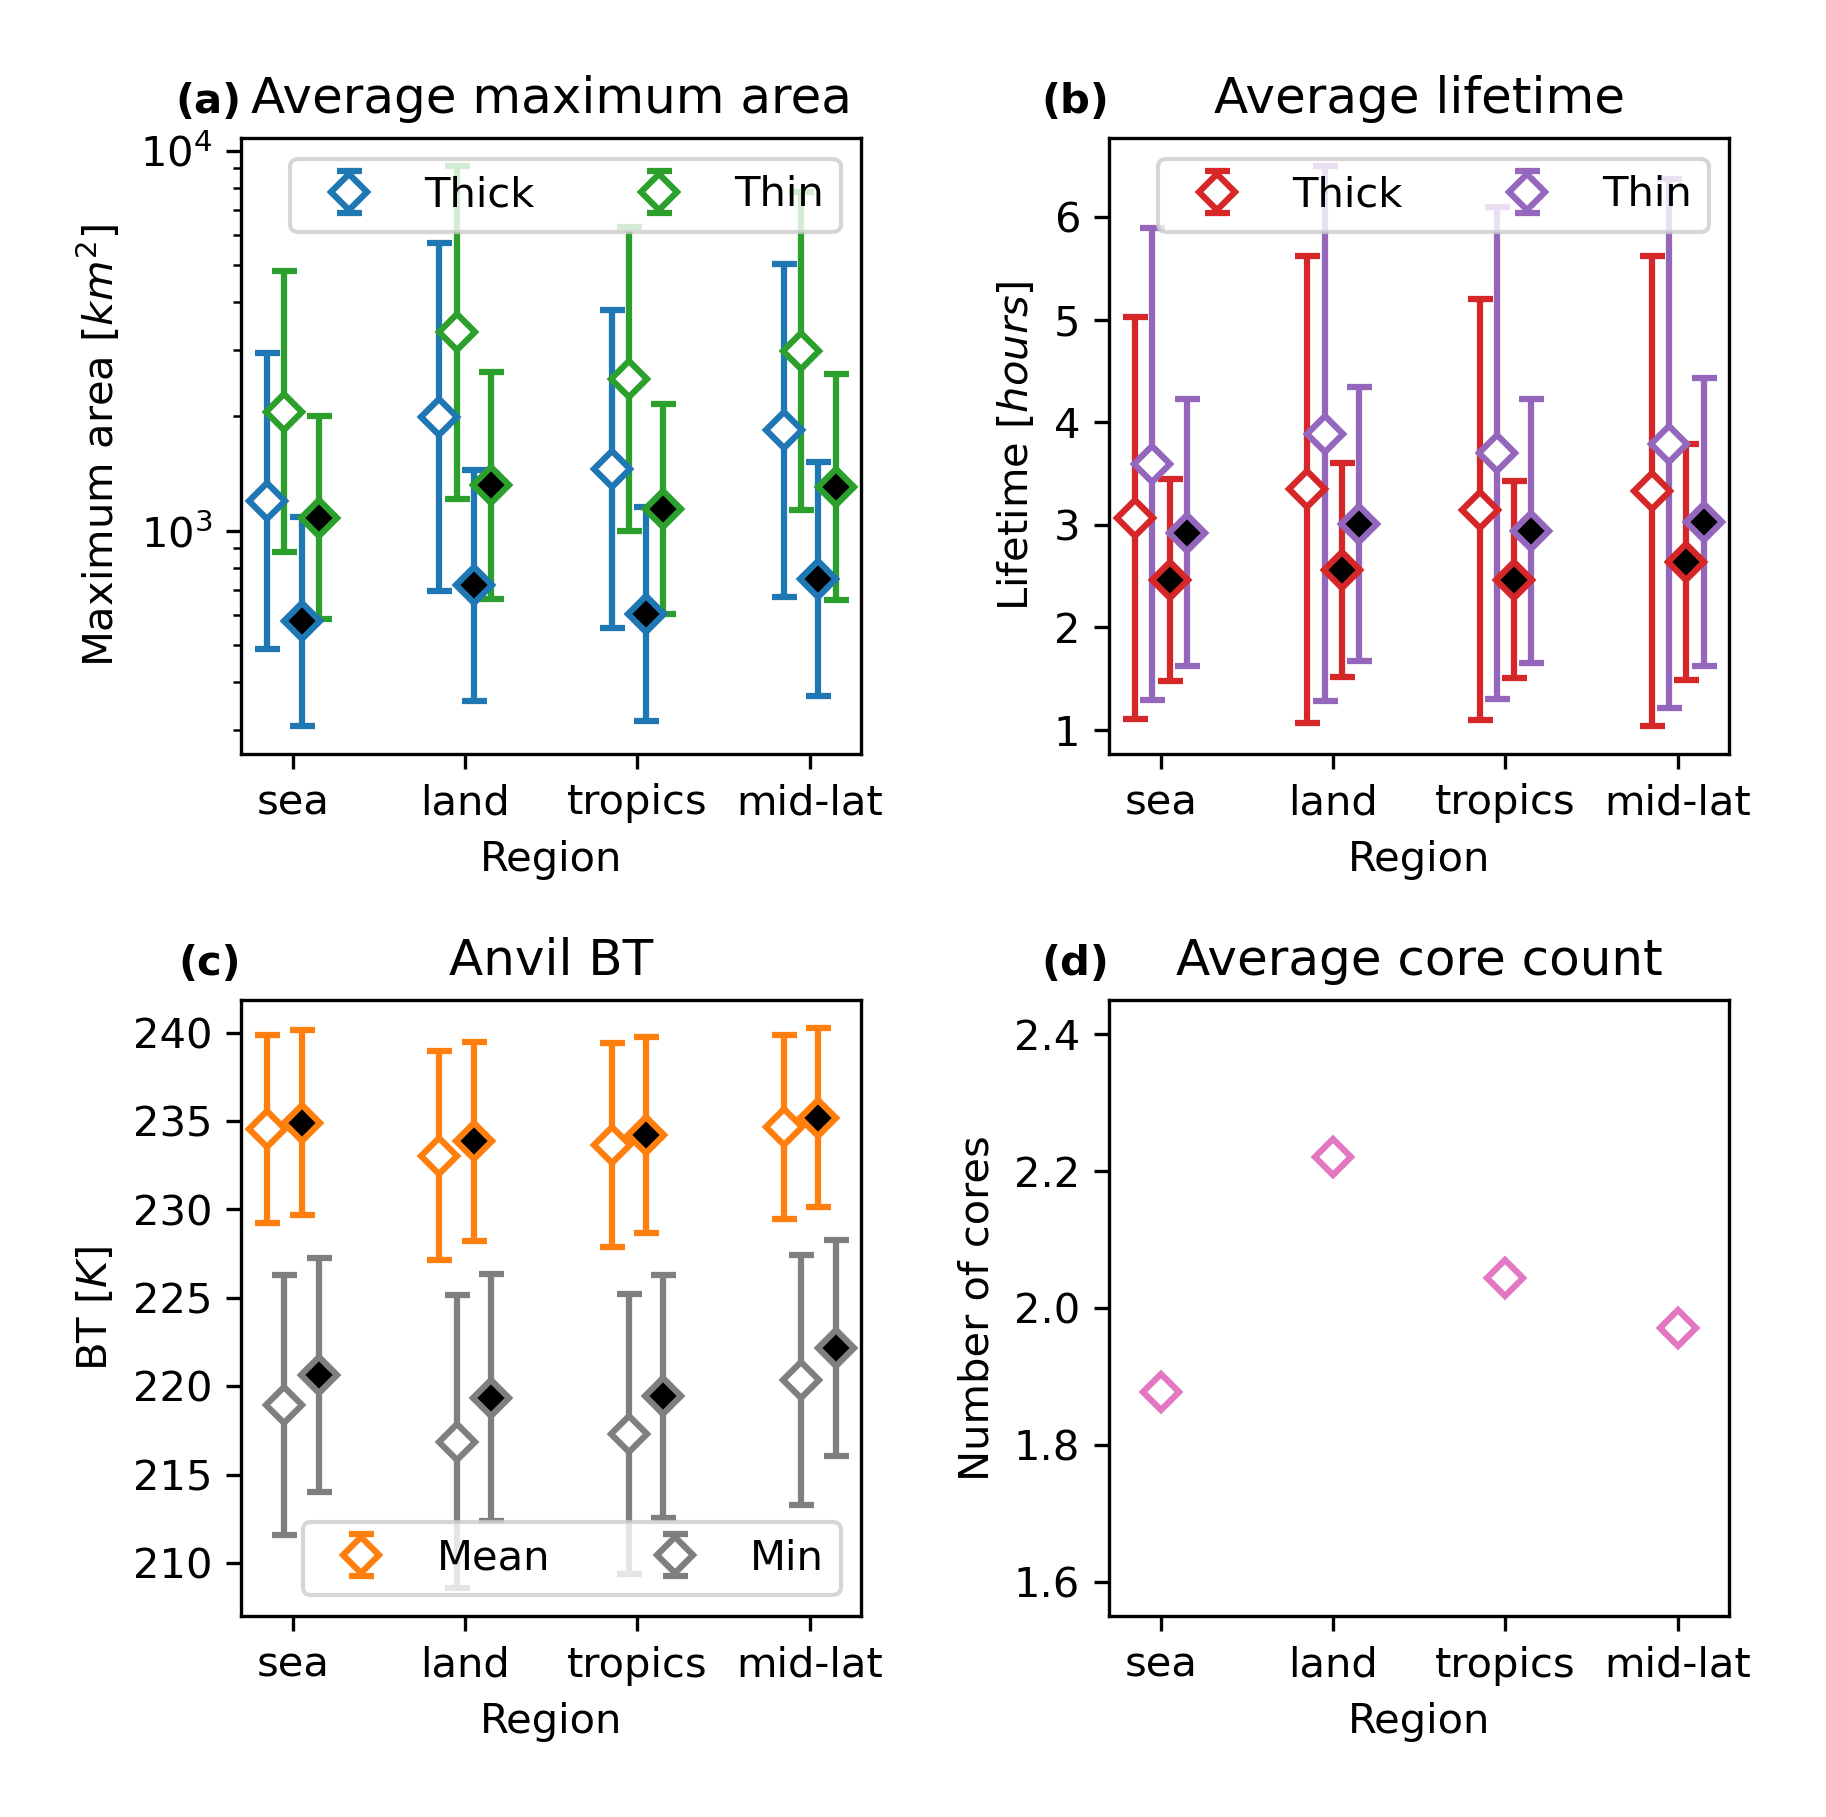
\includegraphics[width=\textwidth]{figures/chapter2_24.png}
    \caption[
    The diurnal distributions of the local time of detection for anvils detected over sea, land, tropics and mid-latitudes
    ]{
    The diurnal distributions of the local time of detection for anvils, binned by hour detected over (a) sea, (b) land, (c) tropics (\textless 30\,\textdegree N) and (d) mid-latitudes (\textgreater 30\,\textdegree N). The hatched area shows the proportion of each distribution associated with multi-core anvils.
    }
    \label{fig:anvil_diurnal_distributions}
\end{figure}

In fig.~\ref{fig:anvil_diurnal_distributions} the diurnal cycles of anvil detections are plotted by region.
The distributions generally match those seen of the core detection times shown in fig.~\ref{fig:core_diurnal_land_sea}, as the majority of the observed anvils are isolated systems.
The diurnal cycle of anvil detections over sea is much less pronounced however, which may lead to the increased variability seen in fig.~\ref{fig:anvil_detection_time_map}.
When comparing the hatched areas, indicating the proportion of the distribution consisting of multi-core anvils, over land, tropics and mid-latitudes the initiation of these organised systems occurs earlier in the day compared to isolated \acrshort{dcc}s.

%f
\begin{figure}[tp]
    \centering
    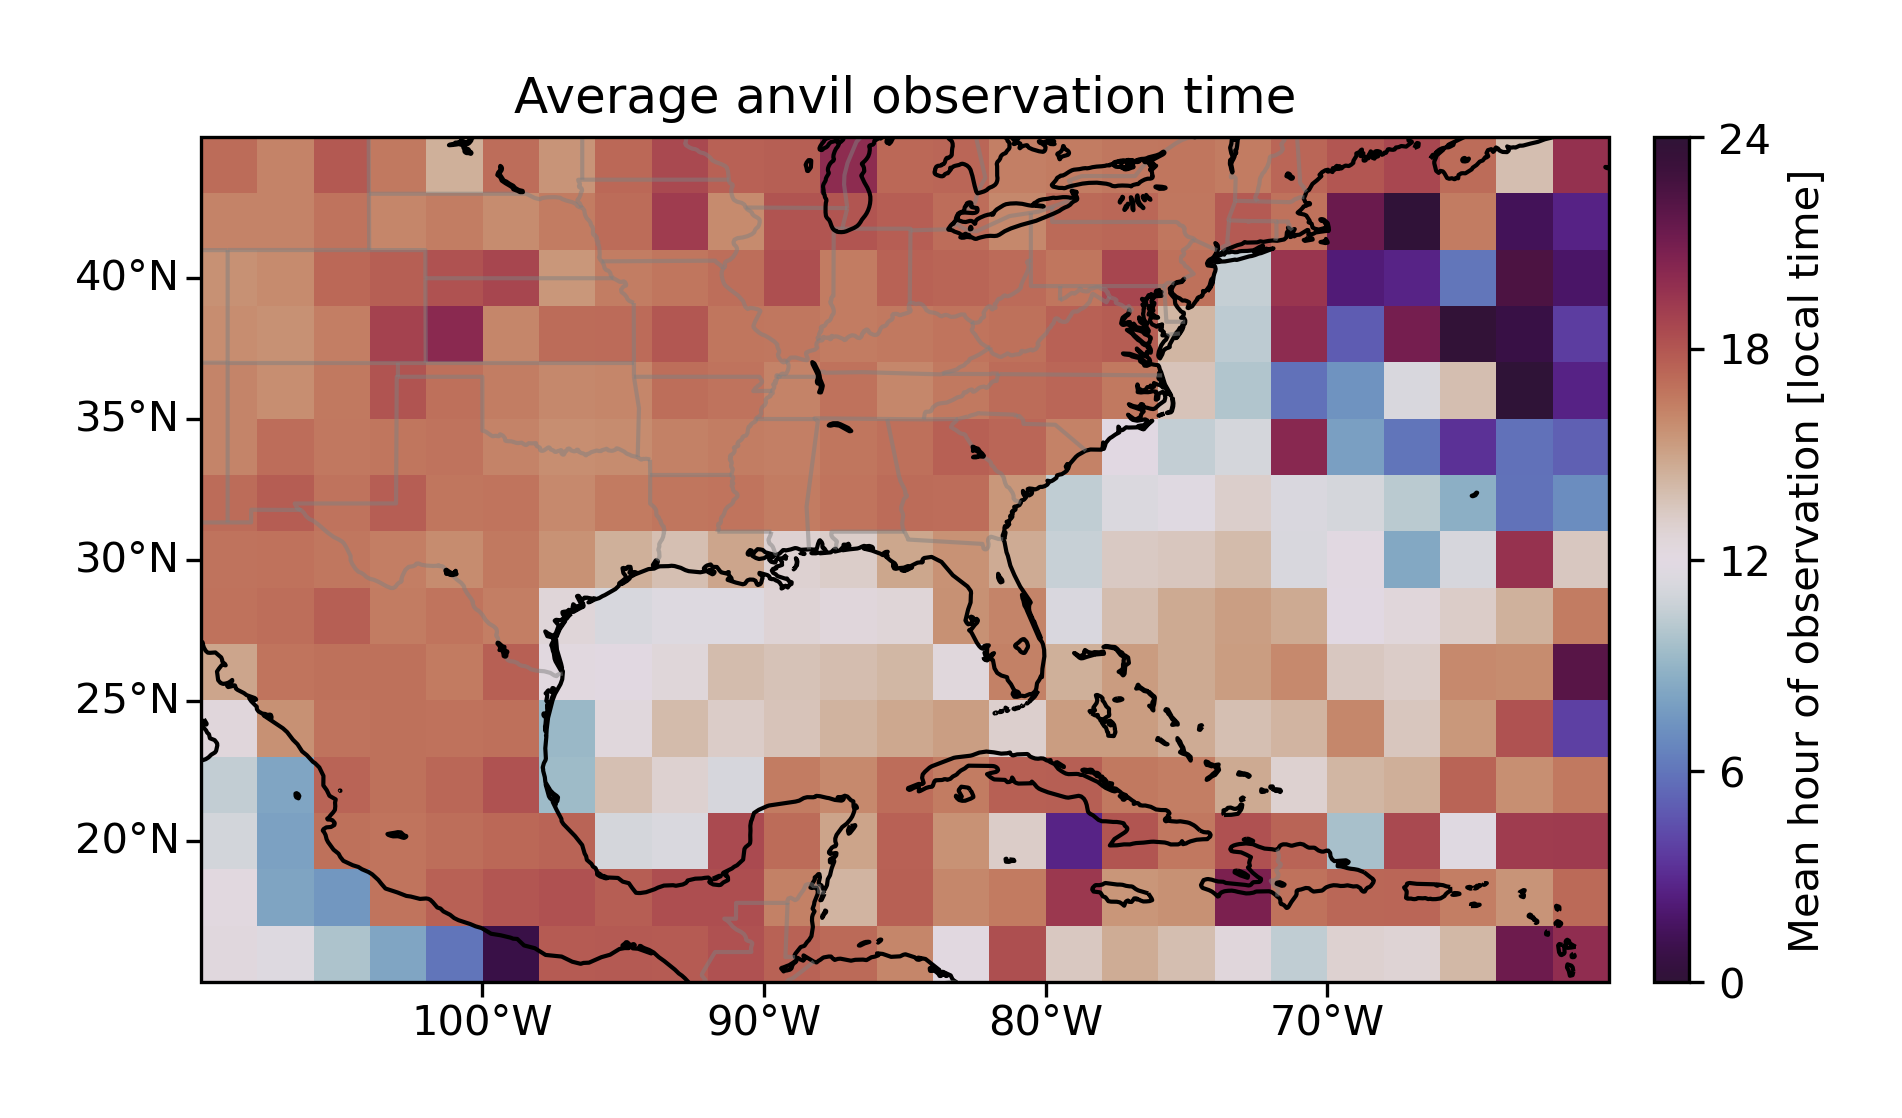
\includegraphics[width=\textwidth]{figures/chapter2_25.png}
    \caption[
    A map showing the average time of observation of anvils
    ]{
    The average time of day of observation of anvils observed within each 2\texttimes2\textdegree\ grid box, calculated as the circular mean of the local solar time. Unlike fig.~\ref{fig:anvil_detection_time_map}, this is the average of the time of observation at every time step along the anvil lifetime.
    }
    \label{fig:anvil_observation_time_map}
\end{figure}

Figure~\ref{fig:anvil_observation_time_map} shows the average time of observation for anvils.
Unlike the previous map of detection time shown in fig.~\ref{fig:anvil_detection_time_map}, in this figure the average of all the time steps at which an anvil is detected is shown.
Over the land, the effect is to shift the timing of the maximum to a later point in the diurnal cycle, which is a shift of approximately half the average anvil lifetime.
Over sea, however, there is a much larger shift with much of the Caribbean showing a similar time of day to adjacent land regions.

%f
\begin{figure}[tp]
    \centering
    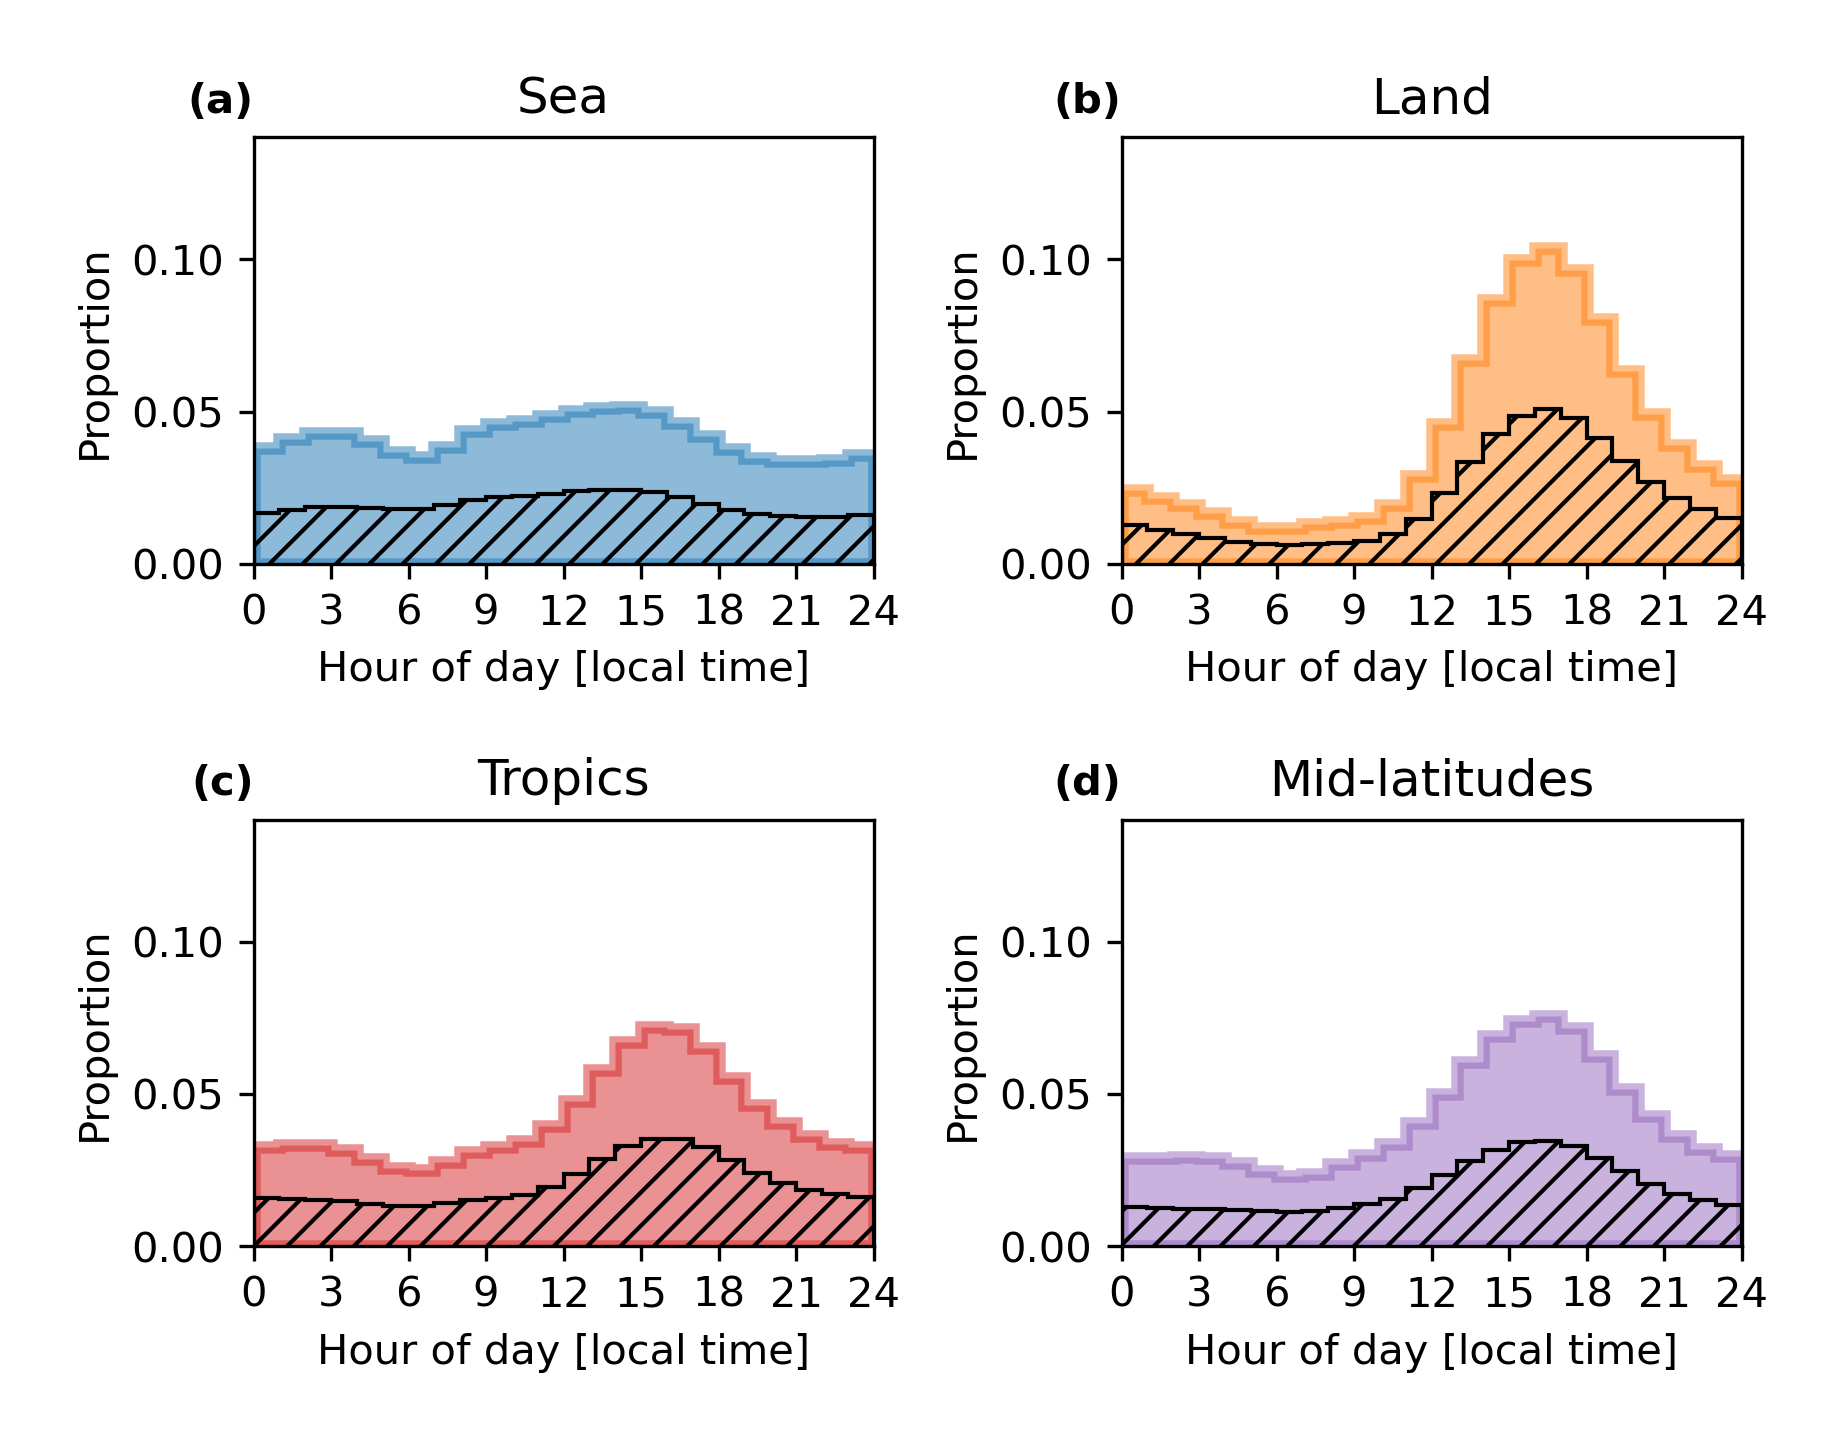
\includegraphics[width=\textwidth]{figures/chapter2_26.png}
    \caption[
    The diurnal distributions of the local time of observation for anvils detected over sea, land, tropics and mid-latitudes
    ]{
    The diurnal distributions of the local time of observation for anvils, binned by hour detected over (a) sea, (b) land, (c) tropics (\textless 30\,\textdegree N) and (d) mid-latitudes (\textgreater 30\,\textdegree N). The hatched area shows the proportion of each distribution associated with multi-core anvils.
    }
    \label{fig:anvil_diurnal_obs_distributions}
\end{figure}

Figure~\ref{fig:anvil_diurnal_obs_distributions} shows the diurnal cycle of anvil observations for each of the four regions.
For the land, tropics and mid-latitudes regions, there is a shift in the peak of the distribution to 4--5\,pm, along with a lengthening of the right tail of the distribution.
The distribution of multi-core anvils appears to match that for all \acrshort{dcc}s.
While in fig.~\ref{fig:anvil_diurnal_distributions} the initiation time of these organised anvils tended to be earlier in the day, their longer lifetime means that they tend to exist, on average, at the same times.
However, this longer lifetime also means that organised \acrshort{dcc}s make up a larger proportion of anvil observations during the nighttime and morning, and fewer during the afternoon during the peak in isolated \acrshort{dcc}s.
In fig.~\ref{fig:anvil_diurnal_obs_distributions}\,a, the peak of the diurnal distribution over the sea is in the afternoon, with a gradual increase of observations throughout the day.
Previous research has shown that solar heating during the daytime increases the area and lifetime of anvils \citep{gasparini_diurnal_2022}, which may explain why there are more anvils observed during the day, despite more initiations occurring at night.

%f
\begin{figure}[tp]
    \centering
    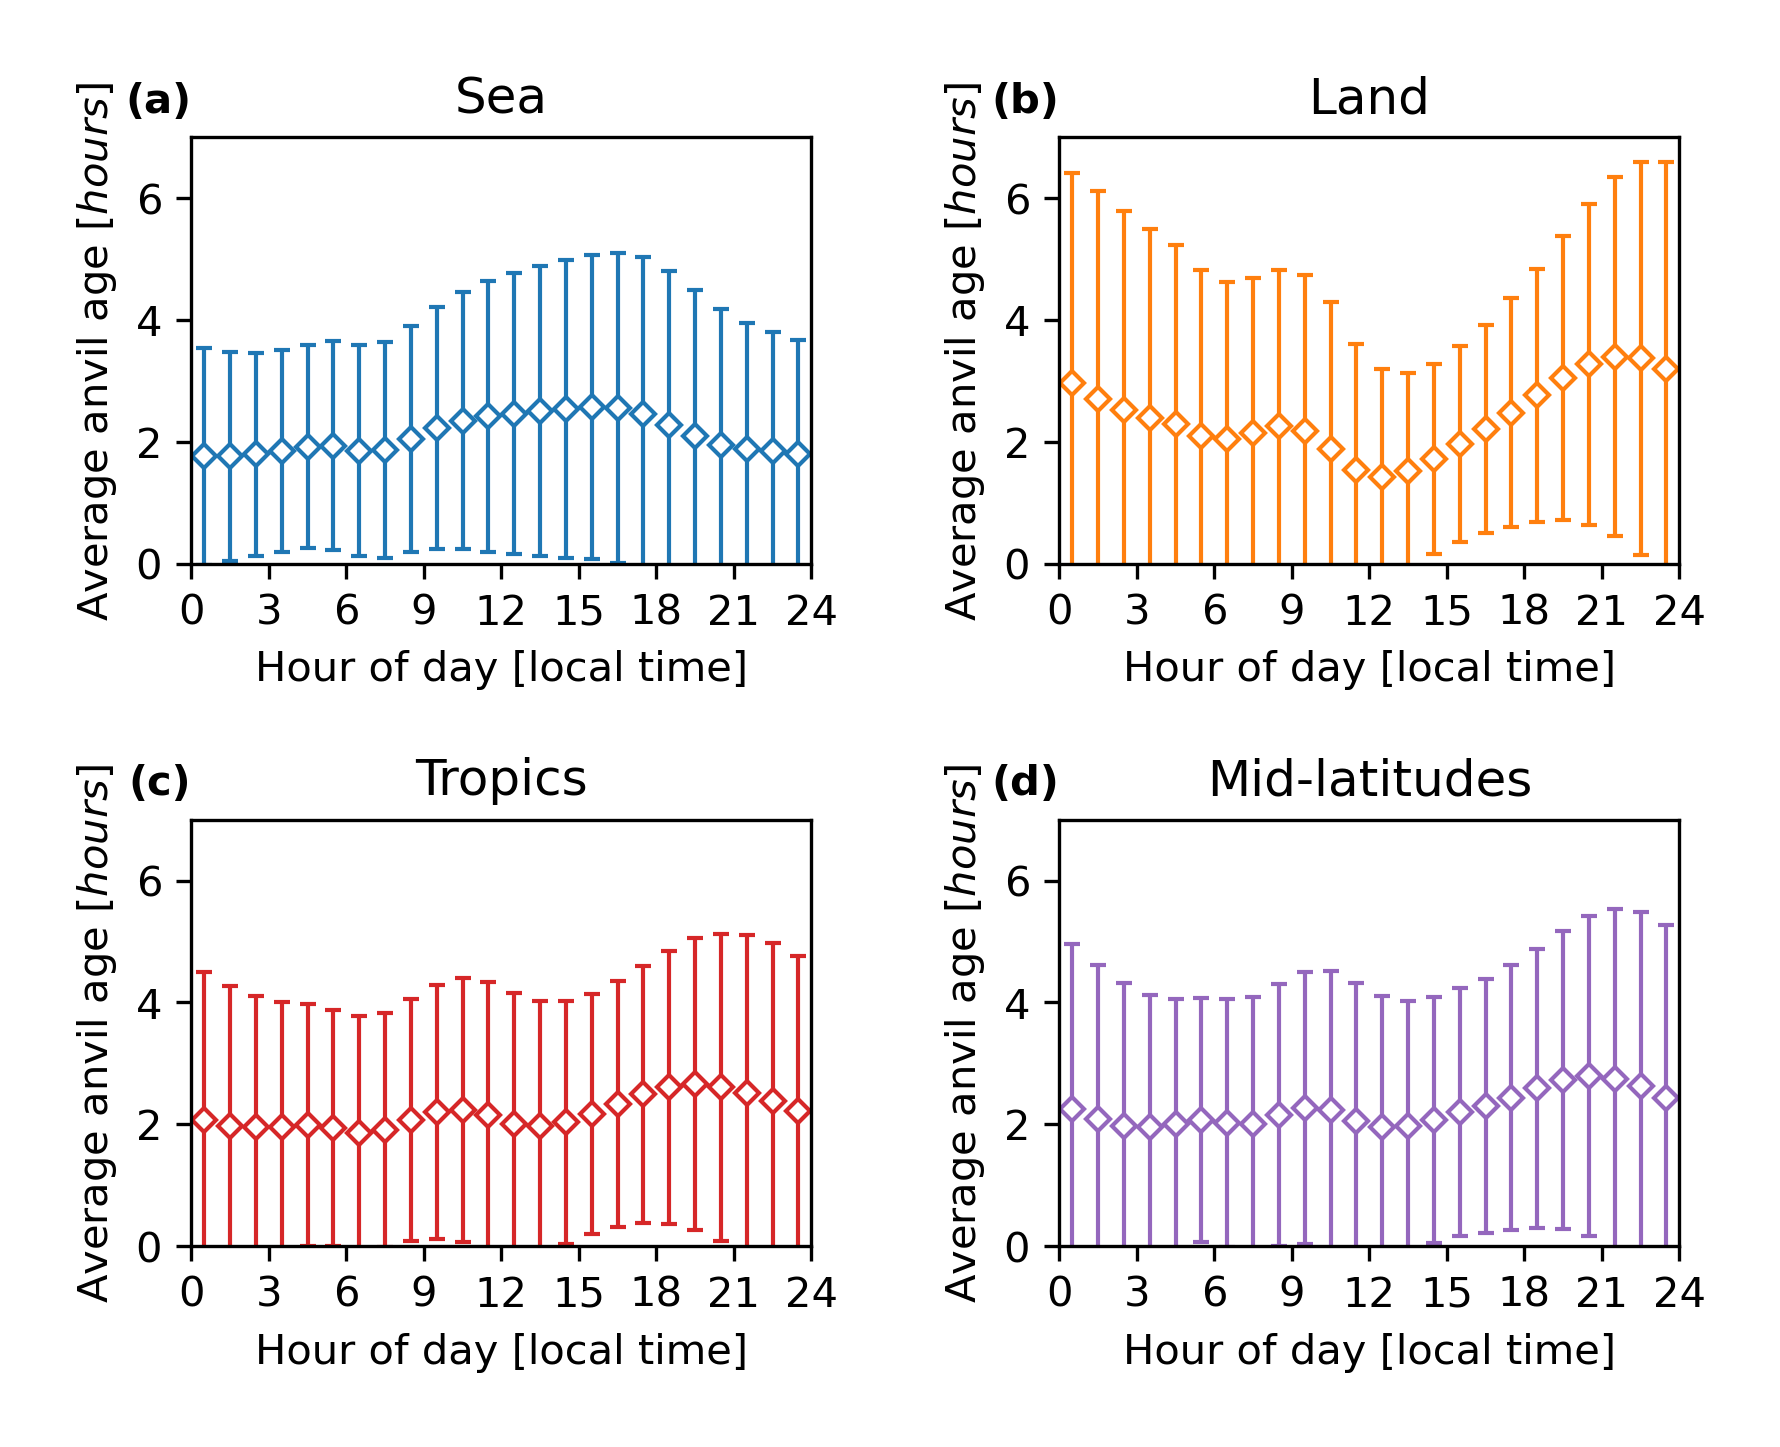
\includegraphics[width=\textwidth]{figures/chapter2_27.png}
    \caption[
    The average age of anvils observed over sea, land, tropics and mid-latitudes throughout the diurnal cycle.
    ]{
    The average age of anvils observed over (a) sea, (b) land, (c) tropics (\textless 30\,\textdegree N) and (d) mid-latitudes (\textgreater 30\,\textdegree N) throughout the diurnal cycle. Error bars show the standard deviation of the mean.
    }
    \label{fig:anvil_diurnal_age}
\end{figure}

The difference in the distributions of anvil initiation times and anvil observation times indicates that the lifetime and age of observed anvils changes across the diurnal cycle.
Figure~\ref{fig:anvil_diurnal_age} shows the average age of anvils observed during each hour of the diurnal cycle.
The increase in the age of anvils observed over sea throughout the daytime provides further evidence for the enhancement of anvil lifetime by \acrshort{sw} radiation.
For anvil observations over land, there is greater interaction with the diurnal cycle of convection.
In fig.~\ref{fig:anvil_diurnal_age}\,b there is a minima of the anvil age between midday and 1\,pm, coinciding with the onset of the afternoon peak of anvil initiations seen in fig.~\ref{fig:anvil_diurnal_distributions}\,b.
The age then increases to a maximum at around 10\,pm, before decreasing again until midday.
The variation in the average age of observed anvils is larger over land than over the ocean.
Over the tropics and mid-latitudes however, the combination of opposite signals from sea and land means that there is much less variation of anvil age across either region.


\section{Summary}  %% \conclusions[modified heading if necessary]

By applying the \textit{tobac-flow} algorithm to five years of multi-channel \acrshort{bt} observations from the \acrshort{goes}-16 \acrshort{abi} \acrshort{conus} scan region, an extensive dataset of \acrshort{dcc} cores and anvils has been produced, including their properties over time.
Containing approximately 1.6 million cores and 400 thousand anvils which are considered valid for analysis over their entire lifecycle, this dataset provides valuable information about their properties, distributions and lifecycle in a Lagrangian framework.
With five-minute temporal resolution, the properties of developing convective cores can be measured accurately, and then linked to the subsequent evolution of the anvil cloud.

A number of key differences in the seasonal, diurnal and regional patterns are seen for \acrshort{dcc}s across North America.
The spatial distribution of \acrshort{dcc} cores depends strongly on the seasonal cycle.
There is a large land/sea contrast in time of initiation, which also displays a sea breeze effect which extends for approximately 200\,\unit{km} inland.
The properties of cores themselves, including the lifetime, cooling rate, and time of initiation, have regional dependencies, with more intense convection occurring over land during the daytime and in the tropics.

These differences extend to the anvils produced by these convective cores.
The seasonal and diurnal cycles of anvils are closely related to those of the convective cores.
Furthermore, there are differences in the properties of anvils between different regions corresponding to differences in convective properties.
In particular, \acrshort{dcc}s over land have larger areas, longer lifetimes and colder \acrshort{bt} than those over the ocean.

While the majority of observed anvil clouds are associated with a single growing core, there are also a large number of multi-core anvils detected in our dataset.
The frequency of multi-core anvils as a proportion of all observed anvils increases with latitude.
Finally, while the properties of the individual growing cores observed in single- and multi-core anvils show no significant difference, the lifetime and area of anvils show a large increase with the number of cores.

Some of these findings, such as the larger area of \acrshort{dcc}s over land, contrast with studies made using polar-orbiting satellites \citep{ge_contrasting_2024}.
However, our investigation of the age of anvils observed throughout the diurnal cycle provides a mechanism for this discrepancy.
The area of \acrshort{dcc} anvils evolves as they age \citep{futyan_deep_2007}.
Impacts of radiative heating and the diurnal cycle act to modify this however \citep{gasparini_diurnal_2022}.
As a result, the average age of observed anvils varies throughout the day.
At the time of the Cloudsat overpass (1:30\,pm), the average age of anvils over land is at its minima, while those over the ocean are near their maxima.
As a result, the average area of anvils observed at this time over land would be smaller than those over the ocean, not because of a difference in their processes but because they are being observed earlier in their lifetime before they have reached their maximum area.
While at the nighttime overpass time (1:30\,am) the average age of anvils over land is older, the reduced number of land \acrshort{dcc}s at this time means that any set of snapshot observations will be biased towards younger anvils over land.

By using temporally resolved observations, and placing these in a Lagrangian framework using cloud tracking, these changes in convective cloud behaviour can be accounted for across the diurnal cycle.
Furthermore, linking the properties of the developing cores to the resulting anvil clouds over their entire lifetime provides the potential to investigate how the processes of the former affect the latter.
Connecting these properties allows investigation of previously uncertain \acrshort{dcc} processes, and, in particular, may help shed light on how anvil optical properties, structure and diurnal cycle respond to climate change.
